\documentclass{classes/fiboThesis}
\usepackage{tabularx}
\usepackage{graphicx}
\usepackage{adjustbox}
\usepackage{lscape}

\begin{document}
\title{Structure Desig and Platform Development of Universal Template\break for Humanoid Algorithm Interface (UTHAI)}
\titleTH{การออกแบบโครงสร้างและพัฒนาระบบพื้นฐานสำหรับหุ่นยนต์ฮิวมานอยด์\break เพื่อการศึกษาและวิจัย}

\author{นายจิรัฏฐ์ ศรีรัตนอาภรณ์}
\authorTwo{นายเจษฎากร ทาไชยวงค์}
\authorThree{นายวุฒิภัทร โชคอนันตทรัพย์}

\majoradvisor{นายธนัชชา ชูพจน์เจริญ}
\coadvisor{รศ.ดร.ชิต เหล่าวัฒนา}
\committeeOne{ดร.อาบทิพย์ ธีรวงศ์กิจ}
\committeeTwo{ดร.ปิติวุฒญ์ ธีรกิตติกุล}
\committeeThree{ดร.สุภชัย วงศ์บุณย์ยง}

\academicyearTH{2560}

\maketitle
\frontmatter
\maketitleinner
\makeapproval
% ************************** Thesis Abstract **********************************
\begin{abstract}
งานวิทยานิพนธ์นี้เป็นงานที่เกี่ยวกับการออกแบบและจัดทำแพลตฟอร์มหุ่นยนต์ฮิวมานอยด์ด้วยเครื่องพิมพ์สามมิติ
โดยใช้ชื่อว่า หุ่นยนต์ฮิวมานอยด์ UTHAI และจุดประสงค์เพื่อให้นักวิจัยท่านอื่นสามารถนำไปพัฒนาต่อได้ง่าย
ภาพรวมของวิทยานิพนธ์นี้จะแบ่งออกเป็นทั้งหมดสามส่วน คือ ส่วนแรกเป็นส่วนของการออกแบบและจัดสร้างส่วนโครงสร้างของหุ่นยนต์ฮิวมานอยด์
ส่วนที่สองเป็นส่วนของการพัฒนาโปรแกรมที่ใช้ในระบบด้วย ROS และส่วนสุดท้ายเป็นส่วนที่ออกแบบระบบพื้นฐานสำหรับการพัฒนาหุ่นยนต์ฮิวมานอยด์
รวมไปถึงมีเอกสาร คู่มือที่อยู่ในรูปแบบออนไลน์
\vfill
\paragraph*{คำสำคัญ :} แพลตฟอร์มหุ่นยนต์ฮิวมานอยด์ / ระบบพื้นฐานหุ่นยนต์ / ROS / เครื่องพิมพ์สามมิติ 
\vfill
\end{abstract}
% ************************** Thesis Acknowledgements **************************
% \majoradvisor{นายธนัชชา ชูพจน์เจริญ}
% \coadvisor{รศ.ดร.ชิต เหล่าวัฒนา}
% \committeeOne{ดร.อาบทิพย์ ธีรวงศ์กิจ}
% \committeeTwo{ดร.ปิติวุฒญ์ ธีรกิตติกุล}
% \committeeThree{ดร.สุภชัย วงศ์บุณย์ยง}
\begin{acknowledgements}
ขอขอบพระคุณอาจารย์ ธนัชชา ชูพจน์เจริญ อาจารย์ที่ปรึกษาวิทยานิพนธ์หลัก
ที่ได้สละเวลามาให้คำปรึกษา ชี้แนะแนวทาง ให้ความรู้ในด้านต่างๆ ที่จำเป็นต่องานวิจัย รวมถึงการให้การสนับสนุนในเรื่องอุปกรณ์ในการทำวิจัย
ตลอดจนช่วยตรวจและแก้ไขวิทยานิพนธ์ให้เป็นไปอย่างสมบูรณ์

ขอขอบพระคุณรองศาสตราจารย์ ดร.ชิต เหล่าวัฒนา อาจารย์ที่ปรึกษาวิทยานิพนธ์ร่วม
ที่ได้ชี้แนะแนวทาง ให้คำแนะนำ และให้เกียรติเข้าร่วมการสอบวิทยานิพนธ์

ขอขอบพระคุณอาจารย์ ดร.ถวิดา มณีวรรณ และนายวิษณุ จูธารี ที่ได้ให้คำแนะนำในการแก้ไขปัญหาด้านต่างๆ
ที่เกิดขึ้นระหว่างการทำการวิจัย และได้ให้การสนับสนุนอุปกรณ์สำคัญที่ใช้ในการทำวิจัย

ขอขอบพระคุณอาจารย์ อาบทิพย์ ธีรวงศ์กิจ ที่กรุณาให้เกียรติเป็นประธานกรรมการสอบวิทยานิพนธ์
ให้คำแนะนำที่เป็นประโยชน์ต่อการจัดทำวิทยานิพนธ์ให้ดำเนินไปอย่างสมบูรณ์

ขอขอบพระคุณอาจารย์ ดร.ปิติวุฒญ์ ธีรกิตติกุล ที่กรุณาให้เกียรติเป็นกรรมการสอบวิทยานิพนธ์ 
ให้คำแนะนำที่เป็นประโยชน์ต่อการวิจัย และการแก้ไขปรับปรุงงานวิจัย ตลอดจนตรวจแก้วิทยานิพนธ์ให้ดำเนินไปอย่างสมบูรณ์

ขอขอบพระคุณอาจารย์ ดร.สุภชัย วงศ์บุณย์ยง ที่กรุณาให้เกียรติเป็นกรรมการสอบวิทยานิพนธ์ 
ให้คำแนะนำที่เป็นประโยชน์ต่อการวิจัย และการแก้ไขปรับปรุงงานวิจัย ตลอดจนตรวจแก้วิทยานิพนธ์ให้ดำเนินไปอย่างสมบูรณ์

ขอขอบพระคุณคณาจารย์ และบุคลากรในสถาบันวิทยาการหุ่นยนต์ภาคสนามทุกท่าน
ที่ได้ให้คำปรึกษาและช่วยเหลือด้านสถานที่พร้อมทั้งสิ่งอำนวยความสะดวกต่างๆ ในระหว่างการทำวิทยานิพนธ์

ขอขอบคุณนักศึกษาปริญญาตรี สถาบันวิทยาการหุ่นยนต์ภาคสนามทุกท่าน
ที่ได้ให้คำแนะนำ ถามไถ่ และเป็นกำลังใจมาโดยตลอด

และสุดท้ายนี้ ขอน้อมรำลึกถึงพระคุณบิดา มารดา และครอบครัว ที่ส่งเสริมให้กำลังใจ
และให้การสนับสนุนในเรื่องต่างๆ จนกระทั่งข้าพเจ้าประสบความสำเร็จในการศึกษา
\end{acknowledgements}

\tableofcontents
\listoffigures
\listoftables
% ***************************** Thesis Symbols ********************************
\begin{symbols}
    \noindent
    \begin{tabular*}{\textwidth}{@{}p{0.18\textwidth}p{0.8\textwidth}@{}}
        {$\theta$} & {เซต้า} \\
        {$d$} & {distance} \\
        {kg} & {Kilogram} \\
        {m$^{2}$} & {Square Metre} \\
    \end{tabular*}
\end{symbols}
% ************************** Thesis Abbreviations **************************
\begin{abbreviations}
    \noindent
    \begin{tabular*}{\textwidth}{@{}p{0.18\textwidth}p{0.8\textwidth}@{}}
        {UTHAI} & {Universal Template for Humanoid Algorithm Interface} \\
        {ROS} & {Robot Operating System} \\
        {IMU} & {Inertial Measurement Unit} \\
        {DoF} & {Degree of Freedom} \\
        {CoM} & {Center of Mass} \\
        {ZMP} & {Zero Moment Point} \\
        {PLA} & {Polylactic acid} \\
        {ABS} & {Acrylonitrile butadiene styrene} \\
        {KMUTT} & {King Mongkut's University of Technology Thonburi} \\
        {Liews} & {วุฒิภัทร โชคอนันตทรัพย์} \\
        {$\theta$} & {เซต้า}
    \end{tabular*}
\end{abbreviations}


\mainmatter
% ************************** Thesis Chapter1 **********************************
\chapter{บทนำ}
\setcounter{page}{1}
\renewcommand{\thepage}{\arabic{page}}
%%%%%%%%%%%%%%%%%%%%%%%%%%%%%%%%%%%%%%%%%%%%%%%%%%%%%%%%%%%%%%%%%%%%%%%%%%%%%%%
\section{ที่มาและความสำคัญ}
% \setlength{\parskip}{0.2em}
หุ่นยนต์ฮิวมานอยด์เป็นหุ่นยนต์ที่สร้างขึ้นเพื่อเลียนแบบสรีระร่างกายของมนุษย์ 
ซึ่งมีข้อจำนวนมากเพื่อให้มีการเคลื่อนไหวคล้ายมนุษย์ ลักษณะเด่นของหุ่นยนต์ฮิวมานอยด์คือ การเคลื่อนที่ด้วยขาสองข้าง
ด้วยการเคลื่อนที่โดยการใช้ขานั้น ทำให้หุ่นยนต์ฮิวมานอยด์สามารถเคลื่อนที่ได้
อย่างคล่องแคล่วในทุกสภาพพื้นผิว ทั้งทางเรียบ ทางขรุขระหรือพื้นต่างระดับ
\footnote{การเคลื่อนที่ของหุ่นยนต์รูปแบบต่างๆ ราชภัฏสวนดุสิต}
ซึ่งนั่นทำให้หุ่นยนต์ที่เดินสองขาแตกต่างจากหุ่นยนต์ที่เคลื่อนที่ด้วยล้อ ด้วยโครงสร้างของหุ่นยนต์ที่คล้ายมนุษย์นั้นเอง 
จึงทำให้หุ่นยนต์ฮิวมานอยด์สามารถทำงานได้หลากหลายและยืดหยุ่น สามารถที่จะใช้อุปกรณ์ทั่วไปที่ถูกออกแบบขึ้นมาเพื่อใช้กับมนุษย์ได้
ซึ่งหมายความว่าในอนาคตนั้นหุ่นยนต์ฮิวมานอยด์สามารถที่จะทำงานทดแทนแรงงานของมนุษย์ได้
\footnote{ณัฐพงษ์ วารีประเสริฐ และณรงศ์ ล่ำดี (2552: 374)}
งานที่หุ่นยนต์ฮิวมานอยด์จะเข้ามาทดแทนแรงงานของมนุษย์นั้น จะเป็นงานที่ต้องทำซ้ำๆ จนเกินความเมื่อยล้า
งานที่อยู่ในพื้นที่อันตรายหรือที่เสี่ยงต่อการเกิดอุบัติเหตุ

สถาบันวิจัยหลายแห่งทั่วโลกกำลังให้ความสนับสนุนด้านการศึกษาวิจัยและพัฒนาหุ่นยนต์ฮิวมานอยด์
เพื่อให้ทำภารกิจต่างๆ ยกตัวอย่างเช่น DARPA Robotics Challenge (DRC)
\footnote{DARPA 2015 [https://www.darpa.mil/about-us/about-darpa]}
เป็นรายการแข่งขันหุ่นยนต์กึ่งอัตโนมัติเพื่อทำภารกิจกู้ภัยในสถานการณ์ภัยพิบัติที่อันตราย
ซึ่งสถาบันวิจัยหุ่นยนต์ทั่วโลกได้ส่งหุ่นยนต์ฮิวมานอยด์ของตนเข้าร่วมการแข่งขัน ในปัจจุบันได้มีการพัฒนาหุ่นยนต์ฮิวมานอยด์ขึ้นมาหลากหลายตัวเช่น
ASIMO, HRP-3, LOLA และ WATHLETE-1 การพัฒนาหุ่นยนต์ฮิวมานอยด์นั้นได้ก่อให้เกิดงานศึกษาวิจัย
และทฏษฏี ต่อยอด ต่างๆมากมาย เช่น
การวางแผนการเดิน การเดินแบบสถิต การเดินแบบพลวัต การติดต่อสื่อสารของระบบ การมองเห็นและการประมวลผลภาพ
การพูดคุยโต้ตอบกับมนุษย์ ปัญญาประดิษฐิ์ ฯลฯ ซึ่งงานวิจัยเหล่านี้สามารถที่จะนำไปประยุกต์ใช้กับระบบหุ่นยนต์ระบบอื่นๆได้ 
แม้ว่าจะมีการพัฒนาหุ่นยนต์ฮิวมานอยด์มามากมายแล้ว แต่การเริ่มต้นทำงานวิจัยที่มีความเกี่ยวข้องกับหุ่นยนต์ฮิวมานอยด์นั้น
ต้องใช้ความรู้ความสามารถ เครื่องมือ ระยะเวลา งบประมาณ และ
ความพยายามเป็นอย่างมาก การสร้างหุ่นยนต์ฮิวมานอยด์ขึ้นมาใหม่นั้นต้องใช้งบประมาณสูง ดั้งนั้นการสร้างระบบจำลองของหุ่นยนต์ฮิวมานอยด์ขึ้นมาเป็นระบบพื้นฐาน 
ให้มีความพร้อมสำหรับการพัฒนาต่อยอดแก่นักศึกษาหรือนักวิจัย จะช่วยประหยัดเวลาและงบประมาณที่ต้องใช้ได้อย่างมาก
ซึ่งนั่นหมายความว่านักวิจัยจะสามารถทำงานวิจัยได้อย่างมีประสิทธิภาพมากขึ้น

ในงานวิจัยนี้เป็นการออกแบบหุ่นยนต์ฮิวมานอยด์และพัฒนาระบบพื้นฐานของหุ่นยนต์ฮิวมานอยด์
สำหรับให้นักศึกษาหรือนักวิจัยสามารถพัฒนาต่อยอดได้ โดยหุ่นยนต์ฮิวมานอยด์ที่ออกแบบมานั้น 
สามารถที่จะปรับปรุง แก้ไข ดัดแปลงได้ง่าย ตัวโครงสร้างจะใช้เป็น พลาสติก PLA ที่สามารถขึ้นรูปได้
โดยการใช้เครื่องพิมพ์สามมิติ มีเซนเซอร์ตรวจการสัมผัสพื้นที่ฝ่าเท้าของหุ่นยนต์ มีเซนเซอร์สำหรับการวัดมุมเอียง
ที่ลำตัวของหุ่นยนต์ และเพื่อที่จะทำให้ง่ายต่อการศึกษาทำความเข้าใจ บำรุงรักษา 
จึงได้มีการจัดทำคู่มือและเอกสารวิธีการใช้งานอย่างชัดเจน โดยจะเก็บในรูปแบบของเอกสารออนไลน์

%%%%%%%%%%%%%%%%%%%%%%%%%%%%%%%%%%%%%%%%%%%%%%%%%%%%%%%%%%%%%%%%%%%%%%%%%%%%%%%
\section{วัตถุประสงค์}
ออกแบบโครงสร้างของหุ่นยนต์ฮิวมานอยด์ที่สามารถแก้ไขปรับเปลี่ยนได้ง่าย พัฒนาระบบพื้นฐาน
ระบบจำลองสำหรับหุ่นยนต์ฮิวมานอยด์เพื่อใช้ในการศึกษาวิจัย รวบรวมเครื่องมือที่เป็นประโยชน์ต่อการพัฒนาหุ่นยนต์ และจัดทำเอกสารออนไลน์
ให้บุคคลที่สนใจสามารถเข้ามาศึกษาได้

%%%%%%%%%%%%%%%%%%%%%%%%%%%%%%%%%%%%%%%%%%%%%%%%%%%%%%%%%%%%%%%%%%%%%%%%%%%%%%%
\section{ประโยชน์ที่คาดว่าจะได้รับ}
\begin{enumerate}[label=\thesection.\arabic*, leftmargin=1.5cm]
	\setlength\itemsep{-0.25em}
	\item มีต้นแบบหุ่นยนต์ฮิวมานอยด์สำหรับใช้ในงานวิจัยแขนงต่างๆ
	\item มีระบบพื้นฐานสำหรับพัฒนาหุ่นยนต์ฮิวมานอยด์รุ่นใหม่ในสถาบัน
	\item มีระบบจำลองสำหรับจำลองการทำงานของหุ่นยนต์ฮิวมานอยด์
	\item มีแหล่งรวบรวมเครื่องมือสำหรับการพัฒนาหุ่นยนต์
	\item มีคู่มือ เอกสาร วิธีการใช้งาน และรายละเอียดของหุ่นยนต์สำหรับพัฒนาต่อยอด
\end{enumerate}

%%%%%%%%%%%%%%%%%%%%%%%%%%%%%%%%%%%%%%%%%%%%%%%%%%%%%%%%%%%%%%%%%%%%%%%%%%%%%%%
\section{ขอบเขตการดำเนินงาน}
\begin{enumerate}[label=\thesection.\arabic*, leftmargin=1.5cm]
	\setlength\itemsep{-0.25em}
	\item ใช้ ROS เป็นกรอบการทำงานสำหรับพัฒนาระบบพื้นฐาน
	\item ออกแบบโครงสร้างให้มีความแข็งแรง สามารถรองรับน้ำหนักอุปกรณ์ที่ติดตั้งอยู่บนตัวหุ่นยนต์ได้
	\item น้ำหนักของหุ่นยนต์รวมกันทั้งตัว ไม่เกิน 5 กิโลกรัม
	\item ใช้ Solidworks 3D เป็นโปรแกรมสำหรับออกแบบโครงสร้าง และคำนวณ
	\item หุ่นยนต์มีความสูงไม่ต่ำกว่า 100 เซนติเมตร และสูงไม่เกิน 120 เซนติเมตร
	\item หุ่นยนต์มี 2 แขน 2 ขา มีองศาอิสระของขาข้างละ 6 และแขนข้างละ 2 องศาอิสระ
	\item หุ่นยนต์สามารถทำงานได้ภายในสภาพแวดล้อมแบบปิด
	\item หุ่นยนต์ใช้พลังงานจากแหล่งจ่ายพลังงานที่มีขนาดแรงดันไฟฟ้า 12 โวลต์
	\item หุ่นยนต์ใช้ตัวขับเคลื่อนแบบดิจิตอลสำหรับแต่ละข้อต่อเป็น Dynamixel Digital Servo
	\item ใช้ Gazebo สำหรับจำลองระบบของหุ่นยนต์
	\item ติดตั้งเซนเซอร์วัดการกด (Ground contact) ที่ฝ่าเท้าของหุ่นยนต์
	\item ติดตั้งเซนเซอร์วัดมุมเอียง (IMU) ที่บริเวณลำตัวของหุ่นยนต์
	\item จัดทำคู่มือ เอกสารการใช้งาน และรายละเอียดส่วนประกอบของหุ่นยนต์
\end{enumerate}

%%%%%%%%%%%%%%%%%%%%%%%%%%%%%%%%%%%%%%%%%%%%%%%%%%%%%%%%%%%%%%%%%%%%%%%%%%%%%%%
\section{ภาพรวมของระบบและขั้นตอนการดำเนินงาน}
งานวิจัยนี้การดำเนินงานวิจัยถูกแบ่งออกเป็นสามส่วน คือ ส่วนที่หนึงส่วนโครงสร้างของหุ่นยนต์ฮิวมานอยด์ เป็นส่วนที่ทำในส่วนของการขึ้นรูปชิ้นงาน
ออกแบบโมเดลสามมิติ รวมไปถึงระบบอิเล็กทรอนิกส์ ติดตั้งบอร์ดและเซนเซอร์ไว้ตามจุดต่างๆ เพื่อสร้างโครงสร้างของหุ่นยนต์ให้สามารถรองรับการเดินได้
ส่วนที่สองส่วนโปรแกรมของหุ่นยนต์ฮิวมานอยด์ เป็นส่วนที่ทำในส่วนของการสั่งการตัวขับเคลื่อนต่างๆ อ่านค่าสถานะเซนเซอร์จากคอนโทลเลอร์
รวมไปถึงระบบจำลองการทำงานของหุ่นยนต์ และส่วนที่สามส่วนการออกแบบระบบพื้นฐานเพื่อการพัฒนาต่อยอด ส่วนนี้จะเป็นส่วนที่ทำให้ผู้ที่จะมาวิจัยต่อยอดสามารถทำงานได้ง่ายขึ้น
จัดการเอกสารคู่มือการใช้งานต่างๆให้เป็นระบบระเบียบ สามารถแยกขั้นตอนการทำงานของแต่ละส่วนออกเป็นข้อดังนี้

\subsection{ส่วนโครงสร้างของหุ่นยนต์ฮิวมานอยด์}
\begin{enumerate}[label=\arabic*, leftmargin=1.5cm]
	\item ศึกษาค้นคว้าเอกสารและงานวิจัยที่เกี่ยวข้อง
	\begin{itemize}
		\setlength\itemsep{-0.3em}
		\item ศึกษาเกี่ยวกับส่วนประกอบของหุ่นยนต์ฮิวมานอยด์
		\item ศึกษาลักษณะกายภาพของมนุษย์
		\item ศึกษาลักษณะกายภาพของหุ่นยนต์ฮิวมานอยด์
		\item ศึกษาการออกแบบฝ่าเท้าและเซนเซอร์ตรวจจับพื้น
		\item ศึกษาการเลือกใช้ตัวขับเคลื่อนและวิธีการไดรว์มอเตอร์
		\item ศึกษาการส่งกำลังไปยังแต่ละข้อต่อ
		\item ศึกษาการออกแบบระบบจ่ายพลังงาน
		\item ศึกษาการใช้งานเซนเซอร์วัดมุมเอียง IMU
	\end{itemize}
	\item ออกแบบโครงสร้างของหุ่นยนต์ฮิวมานอยด์
	\begin{itemize}\setlength\itemsep{-0.3em}
		\item ออกแบบขนาดของหุ่นยนต์
		\item ตรวจสอบความเป็นไปได้ทาง Kinematics
		\item เลือกขนาดของมอเตอร์
		\item ออกแบบการยึดมอเตอร์กับโครงสร้าง
		\item ออกแบบโครงสร้างของหุ่นยนต์
		\item สร้าง CAD Model ของหุ่นยนต์
		\item จำลองและทดสอบความแข็งแรง
		\item ปรับปรุงโครงสร้าง
		\item วางระบบไฟฟ้า
		\item การเลือกใช้แหล่งพลังงาน
		\item การเลือกใช้คอมพิวเตอร์
		\item การไดรว์มอเตอร์
		\item การเชื่อมต่อเซนเซอร์ชนิดต่างๆ
	\end{itemize}
	\item จัดสร้างโครงสร้างหุ่นยนต์ฮิวมานอยด์
	\begin{itemize}\setlength\itemsep{-0.3em}
		\item สั่งซื้อส่วนประกอบทางกล
		\item สั่งซื้อส่วนประกอบทางไฟฟ้า
		\item จัดทำส่วนที่ต้องออกแบบเอง
		\item ประกอบโครงสร้างทางกล
		\item ประกอบโครงสร้างทางไฟฟ้า
	\end{itemize}
	\item ทดสอบการทำงานของหุ่นยนต์ฮิวมานอยด์
	\begin{itemize}\setlength\itemsep{-0.3em}
		\item ทดสอบการเคลื่อนไหวของหุ่นยนต์
		\item ตรวจสอบ Joint limit
		\item ตรวจสอบ Joint frames ทิศทางการหมุน
		\item ตรวจสอบ Kinematics
		\item ทดสอบการขับเคลื่อนของหุ่นยนต์
		\item ตรวจสอบ Power consumption
		\item ทดสอบหารรับรู้ของหุ่นยนต์
		\item ตรวจสอบการอ่านค่าจากเซนเซอร์ IMU
		\item ตรวจสอบการอ่านค่าจากเซนเซอร์ Ground contact
	\end{itemize}

\end{enumerate}

\subsection{ส่วนโปรแกรมของหุ่นยนต์ฮิวมานอยด์}
\begin{enumerate}[label=\arabic*, leftmargin=1.5cm]
	\item ศึกษาค้นคว้าเอกสารและงานวิจัยที่เกี่ยวข้อง
	\begin{itemize}\setlength\itemsep{-0.3em}
		\item ศึกษาระบบที่ใช้ในการพัฒนาหุ่นยนต์
		\item ศึกษาระบบที่ใช้ในการจำลองการทำงานของหุ่นยนต์
	\end{itemize}
	\item ประยุกต์ระบบที่ใช้ในการพัฒนาหุ่นยนต์
	\item ประยุกต์ระบบจำลองการทำงานของหุ่นยนต์
\end{enumerate}

\subsection{ส่วนการออกแบบระบบพื้นฐานเพื่อการพัฒนาต่อยอด}
\begin{enumerate}[label=\arabic*, leftmargin=1.5cm]
	
	\item ติดตั้งระบบ
	\begin{itemize}\setlength\itemsep{-0.3em}
		\item Setup Version Control [GitHub]
		\item ติดตั้ง ROS ในคอมพิวเตอร์ที่อยู่ในหุ่นยนต์
		\item ติดตั้ง ROS ในคอมพิวเตอร์ที่ควบคุมหุ่นยนต์
		\item ตั้งค่า ROS Workspace
		\item ตั้งค่าการติดต่อสื่อสารระหว่างระบบ
	\end{itemize}
	\item วางระบบพื้นฐาน
	% \begin{itemize}\setlength\itemsep{-0.3em}
	% 	\item สร้าง Wiki GitHub
	% 	\item UTHAI-Hardware
	% 	\item UTHAI-Tools
	% 	\item UTHAI-Common
	% 	\item UTHAI-Documents
	% 	\item UTHAI-MPPC
	% 	\item UTHAI-OPC
	% 	\item UTHAI-msgs
	% \end{itemize}
	\item จัดทำคู่มือ
	\begin{itemize}\setlength\itemsep{-0.3em}
		\item รายการของที่จำเป็นต้องใช้
		\item คู่มือการประกอบของหุ่นยนต์
		\item คู่มือรายระเอียดข้อมูลของหุ่นยนต์
		\item คู่มือลิมิตของแต่ละข้อต่อของหุ่นยนต์
		\item คู่มือการวางโครงสร้างของระบบ
	\end{itemize}
	\item สื่อการสอน
	\begin{itemize}\setlength\itemsep{-0.3em}
		\item การติดตั้ง ROS
		\item การใช้งาน ROS เบื้องต้น
		\item การใช้งาน Simulation ของหุ่นยนต์
		\item การใช้งาน ROS กับหุ่นยนต์ฮิวมานอยด์
		\item การใช้งาน ROS บน Mbed
	\end{itemize}
	
\end{enumerate}

%%%%%%%%%%%%%%%%%%%%%%%%%%%%%%%%%%%%%%%%%%%%%%%%%%%%%%%%%%%%%%%%%%%%%%%%%%%%%%%
\clearpage
\section{นิยามศัพท์}
\paragraph*{Gain Pattern}
	% \textbf{Gait Pattern}
คือ รูปแบบการเดินของขาทั้งสองข้างให้เป็นรูปแบบการก้าวเดินเดียวกัน

\paragraph*{Embedded System}
คือ ระบบสมองกลฝังตัว ใช้ในการควบคุมอุปกรณ์ต่างๆ สามารถนำไปใช้ในการควบคุมเฉพาะทาง
การควบคุมแบบแยกส่วน โดยอาศัยตัวประมวลผล ที่ทำหน้าที่วิเคราะห์และประมวลผลข้อมูลตามโปรแกรมที่ได้ออกแบบไว้

% \begin{figure}[htbp]
	\begin{center}
		\begin{tikzpicture}[shorten >=1pt,node distance=2cm,on grid,auto] 
			\node[state,initial] (q_0)   {$q_0$}; 
			\node[state] (q_5) [above right=of q_0] {$q_5$}; 
			\node[state] (q_10) [below right=of q_0] {$q_{10}$};
						
			\node[state,accepting](q_15) [below right=of q_5] {$q_{15}$};
			\node[state,accepting](q_20) [below right=of q_15] {$q_{20}$};
			\node[state] (q_c5) [above right=of q_20] {$qc_{5}$};
			\path[->] 
			(q_0) edge node {5} (q_5)
			edge  node {10} (q_10)
			(q_5) edge node {5} (q_10)
			edge node {10} (q_15)
			(q_10) edge node {5} (q_15)
			edge node {10} (q_20)
			(q_20) edge node {} (q_c5);
			%    edge  node [swap] {1} (q_2)
			% (q_1) 	edge  node  {1} (q_3)
			% 		edge [loop above] node {0} ()
			% (q_2)	edge  node [swap] {0} (q_3) 
			% 		edge [loop below] node {1} ();
		\end{tikzpicture}
		\caption{กราฟแสดงการหยอดเหรียญ 15 Vending Machine}
	\end{center}
\end{figure}
% \section{จลนศาสตร์ของหุ่นยนต์}
จลนศาสตร์ เป็นการศึกษาเกี่ยวกับตำแหน่ง (position), ทิศทางการหมุน (orientation) และการเคลื่อนที่ 
ทั้งเชิงเส้น (translation) และเชิงมุม (rotation) โดยไม่ได้คำนึงถึงแรงที่ก่อให้เกิดการเคลื่อนที่ 
โดยพื้นฐานแล้วหุ่นยนต์เป็นระบบพลวัต (dynamic) ที่เกี่ยวข้องกับการเคลื่อนที่ 
ซึ่งต้องคำนวณถึงแรงที่ก่อให้เกิดการเคลื่อนที่ด้วย
\par
หุ่นยนต์ฮิวมานอยด์ตรงส่วนขา เป็นหุ่นยนต์แบบอนุกรมประกอบขึ้นจากการต่อกันของก้านต่อต่าง ๆด้วยข้อต่อ
ไล่เรียงลำดับจากส่วนสะโพกถึงส่วนปลายเท้า ในลักษณะโครงสร้างแบบโซ่เปิด
ขาของหุ่นยนต์ฮิวมานอยด์จะสามารถเคลื่อนที่ได้ด้วยการขับเคลื่อนของตัวขับ ซึ่งมักติดตั้งอยู่ที่ข้อต่อ 
ซึ่งทำให้ท่าทางของขาถูกกำหนดได้ด้วยค่าตัวแปรของข้อต่อ หากต้องการที่จะรู้ว่าขาของหุ่นยนต์จะเคลื่อนที่
อย่างไรในปริภูมิสามมิติ จำเป็นที่จะต้องรู้ความสัมพันธ์ของตำแหน่งและทิศทางการหมุนของขาหุ่นยนต์ 
และตัวแปรของข้อต่อ
\par
ดังนั้นท่าทางของขาจะถูกกำหนดด้วยค่าตัวแปรของข้อต่อ เพื่อความสะดวกในการใช้งานจึงมักจะ
เขียนให้อยู่ในรูปของเวกเตอร์ เรียกว่าเวกเตอร์ของข้อต่อ (joint vector)

$\dot{q}=[\theta_1 ... \theta_n ]^T$

ปริภูมิของเวกเตอร์ของข้อต่อทั้งหมด จะเรียกว่าปริภูมิของข้อต่อ (joint space)
\par
บางครั้งในทางปฏิบัติ อาจจะมีกลไกบางอย่างเพื่อเปลี่ยนแปลงการเคลื่อนที่จากตัวขับไปยังข้อต่อ 
เพื่อประโยชน์ต่าง ๆ เช่น ทดแรง ทดรอบ ลดมวล นั่นทำให้ ตัวแปรข้อต่อไม่ใช่ตัวแปรที่เกิดจากตัวขับโดยตรง 
จึงมีการเขียนค่าของตัวแปรตัวขับให้อยู่ในรูปของเวกเตอร์ เรียกว่าเวกเตอร์ของตัวขับ (actuator vector)

$\dot{q}=[\theta_1 ... \theta_n ]^T$

ปริภูมิของเวกเตอร์ของตัวขับทั้งหมด จะเรียกว่าเวกเตอร์ของตัวขับ (actuator space)
\par
โดยทั่วไปแล้วการอธิบายส่วนปลายขาของหุ่นยนต์ซึ่งมีทั้งตำแหน่งและทิศทางการหมุน 
นิยมอธิบายด้วยเวกเตอร์ตำแหน่ง และมุมออยเลอร์ โดยเราสามารถเขียนให้อยู่ในรูปเวกเตอร์รวมได้

$\dot{q}=[\theta_1 ... \theta_n ]^T$

ปริภูมิของตำแหน่งและการหมุนนี้จะเรียกว่าปริภูมิของการทำงาน (task space)

จลนศาสตร์ของหุ่นยนต์จะแบ่งออกเป็น 2 ประเภท คือ
\begin{enumerate}[label=\thesection.\arabic*, leftmargin=1.5cm]
	\item จลนศาสตร์ไปข้างหน้า (Forward Kinematics)
จลนศาสตร์ไปข้างหน้าเป็นการวิเคราะห์หาฟังก์ชันของตำแหน่งและทิศทางการหมุน (task space) ในพจน์ที่มีตัวแปรเป็น ค่าของข้อต่อ (joint space)
    \item จลนศาสตร์ผกผัน (Inverse Kinematics)
จลนศาสตร์ผกผันเป็นการวิเคราะห์หาฟังก์ชันของค่าของข้อต่อ (joint space) ในพจน์ที่มีตัวแปรเป็นค่าของตำแหน่งและทิศทางการหมุน (task space)
\end{enumerate}

รูปที่ 2.4 แสดงความสัมพันธ์ระหว่างปริภูมิตัวขับ ปริภูมิข้อต่อ และปริภูมิการทำงาน โดยจลนศาสตร์ไปข้างหน้า


รูปที่ 2.5 แสดงความสัมพันธ์ระหว่างปริภูมิตัวขับ ปริภูมิข้อต่อ และปริภูมิการทำงาน โดยจลนศาสตร์ผกผัน
% \section{การคำนวณพลังงานรวมที่ใช้ของหุ่นยนต์ฮิวมานอยด์}
หุ่นยนต์ฮิวมานอยด์นับเป็นหุ่นยนต์ที่สามารถเคลื่อนที่ได้ ดังนั้นแล้วการบริหารจัดการการใช้พลังงาน 
ย่อมเป็นส่วนสำคัญที่ส่งผลต่อระยะเวลาการใช้งานต่อเนื่อง เพื่อที่จะหาว่าหุ่นยนต์ฮิวมานอยด์ใช้พลังงานไปเท่าใด
ในการทำกิจกรรมบางอย่าง ซึ่งเป็นข้อมูลสำคัญในการกำหนดคุณสมบัติของแบตเตอรี่ 
ภายในระยะเวลาการเดิน 1 คาบ จะใช้พลังงานในการเดินเท่ากับ กำลังของตัวขับทั้ง N ตัวมารวมกัน

$Equation$

โดยที่
 คือ พลังงานที่ใช้ในการเดินหนึ่งคาบ
 คือ กระแสไฟฟ้าของมอเตอร์ที่ 
	 คือ ความต่างศักย์ไฟฟ้าตกคร่อมที่มอเตอร์ที่   
	 คือ เวลา 
 คือ ระยะเวลาของวงจรเดินหนึ่งคาบ 

% % ************************** Thesis Chapter2 **********************************
\chapter{ทฤษฏีและหลักการ}

%% งานวิจัยและทฤษฎีที่เกี่ยวข้อง
\subsection{หุ่นยนต์ฮิวมานอยด์}
หุ่นยนต์ฮิวมานอยด์ คือ หุ่นยนต์ที่ถูกสร้างขึ้นมาให้มีรูปร่างคล้ายคลึงกับสรีระโครงสร้างของมนุษย์
มักถูกออกแบบขึ้นมาเพื่อจุดประสงค์เฉพาะอย่าง เช่น เพื่อให้ใช้เครื่องมือต่างๆของมนุษย์ เพื่อให้อยู่ในสภาพแวดล้อมของมนุษย์
เพื่อศึกษาการเคลื่อนไหนของร่ายกายมนุษย์ เพื่อศึกษาการมองเห็นของมนุษย์ เพื่อทำงานในสิ่งที่มนุษย์ทำได้ยาก
หรือเพื่อวัตถุประสงค์อื่นๆ โดยทั่วไปแล้ว หุ่นยนต์ฮิวมานอยด์จะประกอบไปด้วย 4 ส่วนคือ ส่วนของหัว ส่วนของลำตัว ส่วนของแขน
และส่วนของขา แต่การสร้างหุ่นยนต์ฮิวมานอยด์นั้นก็ไม่จำเป็นที่จะต้องมีส่วนประกอบทุกส่วนดังที่กล่าวไป
ในบางครั้งอาจมีเพียงแค่ส่วนบนเท่านั้น ดังรูปที่ \ref{fig:namo} หุ่นยนต์นะโมจากสถาบันวิทยาการหุ่นยนต์ภาคสนาม
เป็นหุ่นยนต์ที่มีส่วนบนเหมือนมนุษย์ แต่มีส่วนล่างเป็นล้อ หรือหุ่นยนต์ฮิวมานอยด์ที่มีเพียงแค่ส่วนล่าง ดังรูปที่ \ref{fig:ส้มจุก}
หุ่นยนต์ส้มจุก เป็นหุ่นยนต์ฮิวมานอยด์ที่มีเพียงแค่ส่วนขาเท่านั้น หรือหุ่นยนต์ฮิวมานอยด์ที่มีเพียงใบหน้าเหมือนมนุษย์ ดังรูปที่
\ref{fig:โซเฟีย} หุ่นยนต์โซเฟีย เป็นแอนดรอยด์ที่มีหน้าตาคล้ายมนุษย์มาก มีตา มีปาก สามารถพูดปฏิสัมพันธ์กับมนุษย์ได้

\begin{figure}[htbp]
    \centering
    \begin{subfigure}[b]{0.3\textwidth}
        \centering
        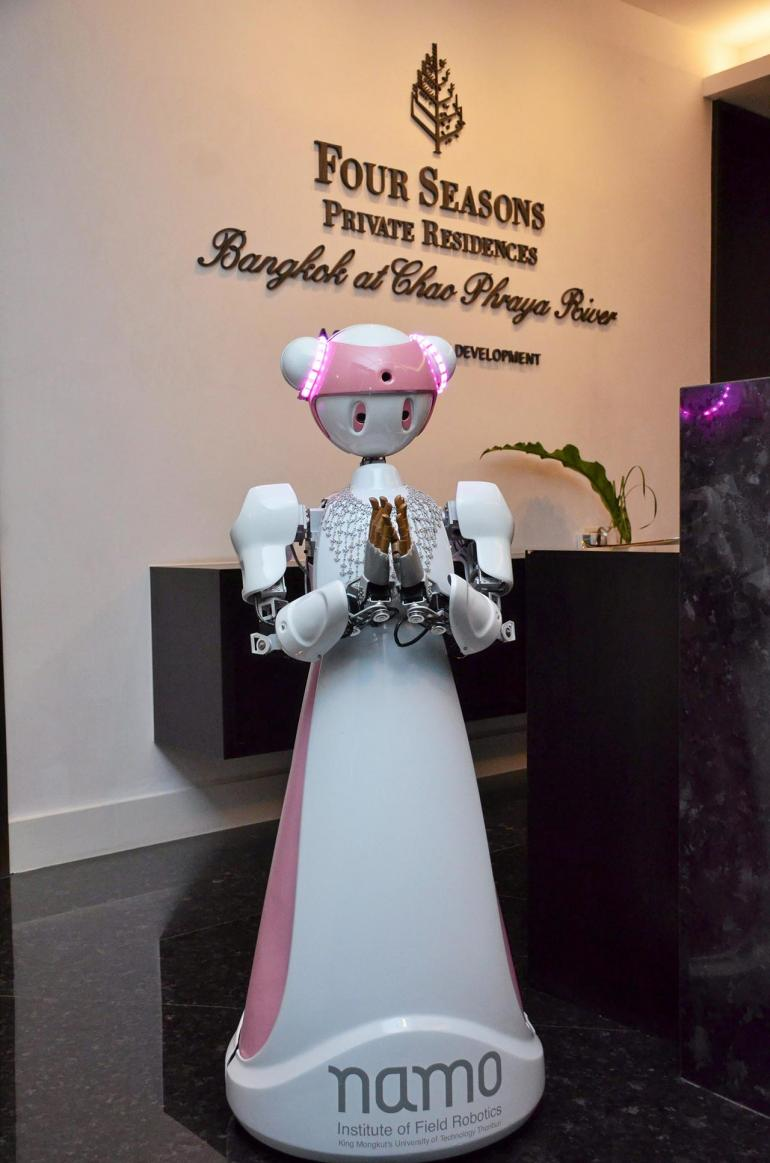
\includegraphics[width=\textwidth]{chapter2/images/namo.jpg}
        \caption{หุ่นยนต์ประชาสัมพันธ์นะโม}
        \label{fig:namo}
    \end{subfigure}
    \hfill
    \begin{subfigure}[b]{0.3\textwidth}
        \centering
        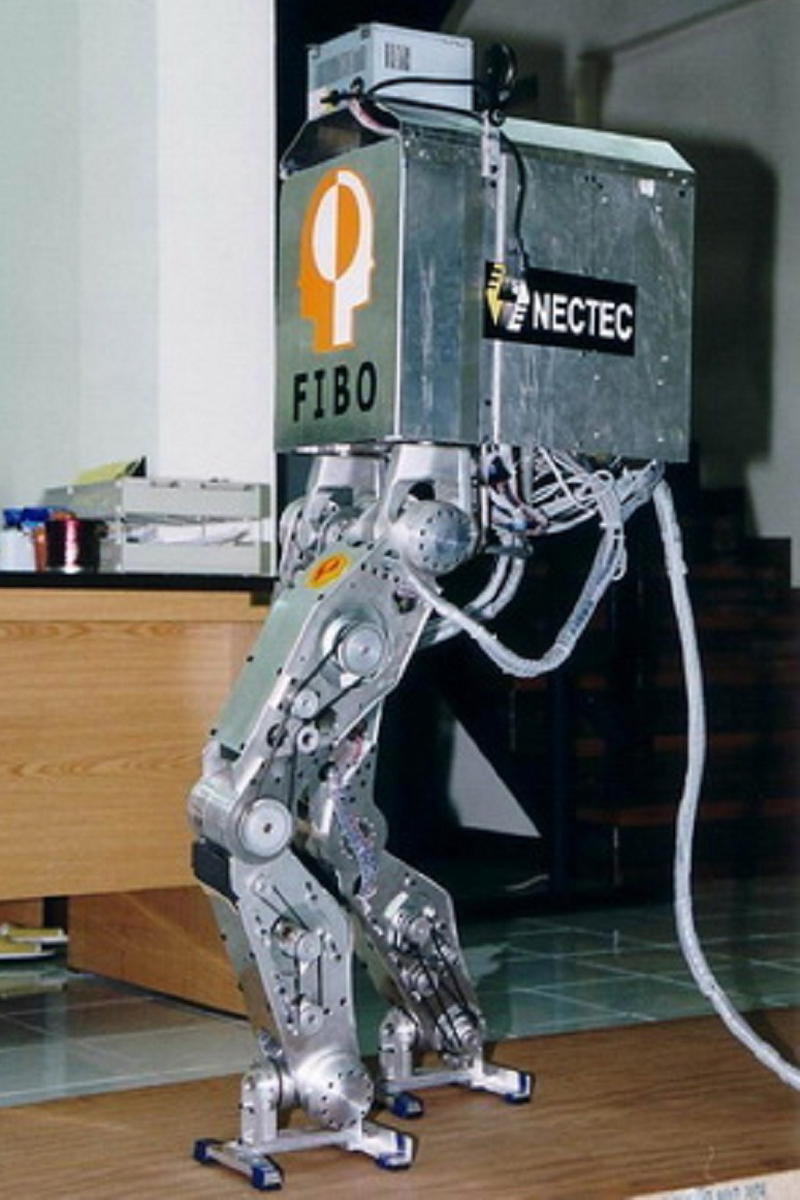
\includegraphics[width=\textwidth]{chapter2/images/ส้มจุก.jpg}
        \caption{หุ่นยนต์เดินสองขาส้มจุก}
        \label{fig:ส้มจุก}
    \end{subfigure}
    \hfill
    \begin{subfigure}[b]{0.3\textwidth}
        \centering
        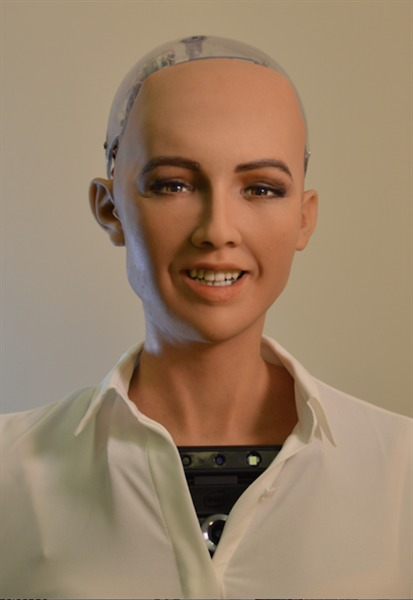
\includegraphics[width=\textwidth]{chapter2/images/โซเฟีย.jpg}
        \caption{หุ่นยนต์แอนดรอยด์โซเฟีย}
        \label{fig:โซเฟีย}
    \end{subfigure}
    \caption{แสดงความแตกต่างของหุ่นยนต์ฮิวมานอยด์แต่ละประเภท}
    \label{fig:diff_humanoid}
\end{figure}

งานวิจัยทางด้านหุ่นยนต์ฮิวมานอยด์จากอดีตจนถึงปัจจุบันส่วนใหญ่จะเป็นการพัฒนาความสามารถของการเดินของหุ่นยนต์
เช่น เริ่มต้นจากแรกสุดจะเป็นการพัฒนาให้หุ่นยนต์สามารถเดินหน้าได้ ต่อมาก็เพิ่มความสามารถให้หุ่นยนต์สามารถเดินบนพื้นเอียง พื้นขรุขระ
เดินเลี้ยวซ้ายขวา เดินขึ้นลงบันได ฯลฯ เป็นต้น นอกจากนี้ยังมีการพัฒนาปรับปรุงสมดุลของการเดินแบบสองขาอีกด้วย สมดุลของการเดินสามารถแบ่งได้สองแบบหลัก
คือ การเดินแบบสมดุลสถิต และการเดินแบบสมดุลพลวัต งานในยุคแรกนั้นจะพัฒนาให้เดินได้แบบสมดุลสถิต ต่อมาเป็นสมดุลกึ่งพลวัต
และเป็นสมดุลพลวัต การพัฒนาตัวควบคุมการเดินของหุ่นยนต์ จำเป็นที่จะต้องใช้ความรู้ทางด้านกลศาสตร์ค่อนข้างมาก มีการใช้สมการที่มีความซับซ้อน

Zheng และคณะ (1988) พัฒนาหุ่นยนต์สองขาที่สามารถเดินบนพื้นราบได้ ให้สามารถเดินต่อเนื่องไปบนพื้นเอียงได้ด้วย
พื้นเอียงที่ใช้มีลักษณะเป็นพื้นเอียงขึ้น หุ่นยนต์ที่ใช้ในงานนี้มีข้อต่อสะโพก (hip), ข้อเท้า (ankle) และลำตัว (torso) มีเซนเซอร์วัดแรงกด (force sensor)
ติดตั้งอยู่ที่ปลายเท้าและส้นเท้าแต่ละข้างเพื่อใช้วัดตำแหน่งของน้ำหนักโดยรวม (center of gravity) ของหุ่นยนต์ การเดินของงานวิจัยจะพิจารณาเฉพาะการเดินในแนวหน้าหลัง
โดยมีหลักการคือ การเดินบนพื้นเอียงโดยที่หุ่นยนต์ยังเดินในท่าทางเหมือนกับตอนที่เดินบนพื้นราบจะทำให้น้ำหนักโดยรวมของหุ่นยนต์เลื่อนไปข้างหลัง
ดังนั้นการที่หุ่นยนต์ขยับลำตัวไปด้านหน้าจำทำให้น้ำหนักโดยรวมของหุ่นยนต์กลับมาอยู่ตรงกลางของพื้นที่รับน้ำหนักเหมือนเดิม
ซึ่งจะทำให้หุ่นยนต์มีความสมดุลได้ ดั้งนั้นข้อมูลที่ได้จากหน่วยวัดแรงกดที่เท้าจะถูกนำมาคำนวณตลอดการเดินเพื่อใช้ในการปรับเปลี่ยนมุมการขยับของลำตัว
การเดินบนพื้นราบเป็นแบบสมดุลสถิตและการเดินบนพื้นเอียงก็ยังคงเป็นแบบสมดุลสถิตเช่นกัน

Inaba และคณะ (1995) สร้างหุ่นยนต์เลียนแบบลิง (ape-like biped) ประกอบด้วยสองมือและสองขา มีการเดินแบบสมดุลสถิต
งานวิจัยนี้มีความคิดว่านอกจากการทำให้หุ่นยนต์สองขาเดินได้โดยไม่ล้มแล้ว ควรจะทำหุ่นยนต์ที่สามารถลุกขึ้นเองได้หลังจากที่ล้มแล้วด้วย
ดังนั้นในงานนี้ หุ่นยนต์ถูกพัฒนาให้สามารถเดิน เมื่อล้มแล้วก็สามารถพลิกตัวและลุกขึ้นมาเดินให้ได้

Kun และ Miller (1996) ได้นำโครงข่ายประสาทเทียม มาประยุกต์ใช้ในการปรับเปลี่ยนท่าทางการเดินโดยอัตโนมัติของหุ่นยนต์สองขา
การที่หุ่นยนต์สามารถปรับเปลี่ยนท่าทางได้โดยอัตโนมัตินี้มีประโยชน์ทำให้หุ่นยนต์เดินได้บนพื้นผิวหลากหลายลักษณะมากขึ้น
ในงานนี้พิจารณาท้ังสมดุลในแนวหน้าหลัง (sigittal plane) และแนวซ้ายขวา (frontal plane) และการเดินของหุุ่นยนต์เป็นแบบสมดุลพลวัต
หลักการทำงานประกอบด้วยตัวสร้างท่าทางการเดินหนึ่งตัว และตัวปรับท่าทางการเดินทั้งแนวหน้าหลังและซ้ายขวาอีกหนึ่งตัว
โดยค่าการปรับเปลี่ยนนั้นจะได้มาจาก แรงกดที่เท้า ความยาวการก้าวเท้า ความสูงของการยกเท้า เป็นต้น นอกจากนี้
ในปีถัดมาทั้งสิงได้ใช้หลักการที่ใช้ในงานนี้ไปใช้กับการเดินของหุ่นยนต์อีกตัว (Kun and Miller, 1997)

Hirai และคณะ (1998) พัฒนาหุ่นยนต์ฮิวมานอยด์ ซึ่งตัวหุ่นยนต์มีความคล้ายมนุษย์มาก สามารถเดินได้อย่างราบลื่นคล้านมนุษย์มากที่สุด
เช่น สามารถเดินได้ในพื้นผิวชนิดต่างๆ เดินได้บนพื้นเอียงขึ้นเอียงลง เดินขึ้นลงบันได้ได้ เดินเข็นรถได้ เป็นต้น การเดินในทุกสถานการณ์เป็นการเดินแบบสมดุลพลวัต
หุ่นยนต์สามารถเดินได้ด้วยความเร็วสูงสุด 4.7 กิโลเมตรต่อชั่วโมง หุ่นยนต์ประกอบไปด้วย แขนข้างละ 9 องศาอิสระ ขาข้างละ 6 องศาอิสระ
ที่บริเวณหัวมีกล้องติดตั้งอยู่ 4 ตัว นอกจากนี้ยังมีอุปกรณ์ที่ใช้ในการรักษาสมดุลอื่นๆ อีกได้แก่ IMU ที่ติดตั้งบริเวณลำตัว และ Force sensor ที่ติดที่เท้าทั้งสองข้าง

\clearpage
ส่วนประกอบของหุ่นยนต์ฮิวมานอยด์สามารถจำแนกออกเป็นส่วนหลักๆได้สามส่วนคือ 
ส่วนการรับรู้ ส่วนการประมวลผล และส่วนการขับเคลื่อน

\subsubsection*{การรับรู้ของหุ่นยนต์ฮิวมานอยด์}
การรับรู้ของหุ่นยนต์ฮิวมานอยด์นั้นมีความยากมากกว่าหุ่นยนต์ชนิดอื่นๆเพราะหุ่นยนต์จะมีการเคลื่อนที่ และการเคลื่อนที่นั้นทำให้เซนเซอร์โดนรบกวนได้
ยกตัวอย่างเช่น ภาพที่ได้จากกล้องนั้นอาจจะเบลอได้ถ้าความเร็วของชัตเตอร์ช้าเกินไป หรือว่าภาพเปลี่ยนขณะที่กำลังกดชัตเตอร์
ข้อมูลตำแหน่งของตัวเองก็มีความแน่นอนที่น้อยกว่าหุ่นยนต์เคลื่อนที่ด้วยล้อ เพราะเซนเซอร์ที่วัดตำแหน่งเทียบกับเฟรมโลกไม่มีความเสถียร
หุ่นยนต์ที่เคลื่อนที่ด้วยล้อปกติถ้าติดกล้อง ตัวกล้องจะมีความสูงจากพื้นคงที่ แต่หุ่นยนต์ฮิวมานอยด์ไม่ใช่ โดยหุ่นยนต์ฮิวมานอยด์นั้นจะต้องมีการคำนวณ
forward kinematics จากเท้าที่สัมผัสกับพื้นมายังกล้องเพื่อหาตำแหน่งและการหมุนของกล้อง ส่วนการวัดตำแหน่งของตัวหุ่นยนต์นั้น
โดยทั่วไปแล้วจะใช้เซนเซอร์ inertia measurement unit (IMU) และเซนเซอร์ Encoders สำหรับหาตำแหน่งของข้อต่อต่างๆ
ปกติจะติดเซนเซอร์ IMU ไว้ที่ลำตัวของหุ่นยนต์ใกล้ๆกับ center of mass ของหุ่นยนต์ ส่วน Encoder นั้นจะติดไว้ที่ข้อต่อของหุ่นยนต์

\subsubsection*{การประมวลผลของหุ่นยนต์ฮิวมานอยด์}
ในปัจจุบันนี้หุ่นยนต์ฮิวมานอยด์มีความสามารถในการคำนวณที่สูงมากเมื่อเทียบกับเมื่อก่อน บอร์ดที่เราสามารถเห็นได้โดยทั่วไปเช่น
Raspberry Pi, Odroid, Intel NUCs ซึ่งตัวบอร์ดมีขนาดเล็กจึงทำให้เข้าไปอยู่ในตัวของหุ่นยนต์ได้ แถมบอร์ดพวกนี้ยังมี GPUs
และ CPU หลายคอร์อีกด้วย บางครั้งก็มีคนที่เอาพวกบอร์ดพวกนี้มาทำงานร่วมกันหลายๆตัว ประมวลผลแบบ pararell เพื่อที่จะเพิ่มประสิทธิภาพในการประมวลผล
โดยเชื่อมต่อระหว่างกันผ่าน Ethernet network 

\subsubsection*{การขับเคลื่อนของหุ่นยนต์ฮิวมานอยด์}
หุ่นยนต์ฮิวมานอยด์ส่วนใหญ่จะมีข้อต่ออยู่หลายๆจุด แต่ละข้อต่อจะมีตัวขับเคลื่อน ตัวขับเคลื่อนมีอยู่หลักๆสองแบบคือ
แบบกล้ามเนื่อของมนุษย์ และแบบมอเตอร์ที่ติดตรงที่ข้อต่อเลย ที่นิยมใช้คือแบบมอเตอร์ที่ติดที่ข้อต่อเลย เพราะทำให้ตัวของหุ่นยนต์มีขนาดเล็ก
ใช้พื้นที่น้อย การใช้เส้นเอ็นดึงนั้นจะการจะทำให้ข้อต่อไปยังตำแหน่งที่ต้องการได้ยากกว่า ตัวขับเคลื่อนนั้นต้องการแรงมากน้อยขึ้นอยู่กับ
น้ำหนักของตัวหุ่นยนต์ เพื่อที่จะทำให้หุ่นยนต์นั้นยังยืนได้

\clearpage
\subsection{ทฤษฏีที่เกี่ยวข้องกับมนุษย์}
\subsubsection{การวิเคราะห์การเดินของมนุษย์}
การเคลื่อนที่ของหุ่นยนต์ฮิวมานอยด์นั้นจะเลียนแบบมาจากการเดินของมนุษย์
ดั้งนั้นการวิเคราะห์ลักษณะการเดินของมนุษย์ จะเป็นการศึกษาเพื่อทำความเข้าใจถึงธรรมชาติการเดิน
ก่อนนำไปทำการออกแบบกลไกทางกลและระบบควบคุมของหุ่นยนต์ฮิวมานอยด์
การก้าวเดินของมนุษย์โดยปกติแล้ว จะมีลักษณะเป็นวัฏจักร วนซ้ำไปเรื่อยๆ ในทิศทางที่ต้องการจนกว่าจะทำการหยุดเดิน
การทรงตัวในระหว่างการยืนหรือการเดินนั้น เป็นไปตามสัญชาติญาณซึ่งเกิดจากการรักษาความสมดุลของระดับน้ำในหู\footnote{text}
ส่งสัญญาณผ่านเส้นประสาทไปยังกล้ามเนื้อส่วนต่างๆ ที่ทำหน้าที่ให้เกิดการเคลื่อนที่

การเคลื่อนที่ของมนุษย์ในการเดินไปข้างหน้าสามารถแบ่งออกเป็นช่วงต่างๆดังนี้
\begin{figure}[htbp]
    \centering
    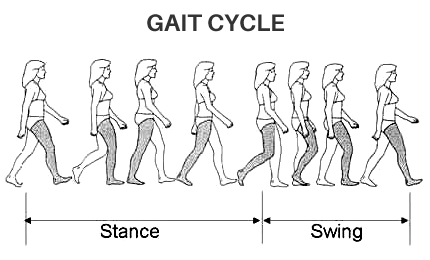
\includegraphics[width=0.55\textwidth]{chapter2/images/gaitcycle.png}
    \caption{วัฏจักรการเดินของมนุษย์}
    \label{fig:human_gait_cycle}
\end{figure}
\begin{enumerate}[label=\arabic*., leftmargin=1.5cm]
    \item ช่วงเริ่มการวางเท้าเพื่อเข้าสู่ช่วงเริ่มต้นเหวี่ยงเท้า เป็นช่วงที่เท้าเกิดการกระแทกลงบนพื้นหลังจากทำการเหวี่ยงมาจากด้านหลัง
    โดยธรรมชาติมนุษย์จะทำการวางส้นเท้าลงเพื่อลดแรงกระแทกที่เกิดขึ้นในช่วงนี้
    ดังนั้นทางกายภาพในส่วนของส้นเท้ามนุษย์จึงมีลักษณะอ่อนนุ่ม
    \item ช่วงเริ่มต้นเหวี่ยงเท้าเพื่อเข้าสู่ช่วงเหวี่ยงเท้า หลังจากทำการวางส้นเท้าลงกับพื้นแล้ว ข้อเข้าจะปรับมุมเพื่อให้ฝ่าเท้าแนบพื้นสนิท
    ขณะเดียวกันขาอีกข้างจะยกสูงขึ้นเพื่อถ่ายเทน้ำหนักไปยังเท้าที่เพิ่งวางลง
	\item ช่วงเหวี่ยงเท้า เป็นช่วงที่ขาหนึ่งยกลอยอยู่ในอากาศและขาที่วางแนบกับพื้นจะรองรับน้ำหนักทั้งหมดของร่างกาย
	\item ช่วงเตรียมการวางเท้า เป็นช่วงที่ขาข้างที่ลอยอยู่เหวี่ยงไปข้างหน้าเพื่อเตรียมเข้าสู่ช่วงรองรับ 
    ในขณะเดียวกันขาที่รับน้ำหนักอยู่จะทำการผลักตัวเพื่อเริ่มทำการถ่ายเทน้ำหนักไปข้างหน้า
\end{enumerate}

\subsubsection{การวิเคราะห์องศาอิสระของมนุษย์}
การที่มนุษย์เราสามารถเคลื่อนที่ได้นั้น เป็นผลเนื่องมาจากการเคลื่อนที่ของข้อต่อต่าง ๆ ที่อยู่
บนขา ซึ่งประกอบไปด้วย ข้อต่อส่วนสะโพก ข้อต่อส่วนหัวเข่า และข้อต่อส่วนข้อเท้า แรงบิดที่เกิด
ขึ้นของแต่ละข้อต่อมีความสัมพันธ์ต่อกัน ส่งผลให้เกิดเสถียรภาพในการเดินของมนุษย์ เมื่อวิเคราะห์
ลักษณะโครงสร้างในแต่ละส่วน พบว่าข้อต่อส่วนสะโพกมีลักษณะเป็นทรงกลม ทำให้ข้อต่อส่วน
สะโพกสามารถหมุนได้ 3 องศาอิสระ ส่วนหัวเข่าของมนุษย์ มีจุดต่อของข้อที่มีลักษณะเป็นทรงกลม
สองลูกประกอบเข้าด้วยกันทำให้การเคลื่อนที่ถูกบังคับให้สามารถเคลื่อนที่ได้เพียง 1 องศาอิสระ ใน
ส่วนของข้อเท้ามีลักษณะการเคลื่อนที่เหมือนสะโพกคือสามารถเคลื่อนที่ได้ 3 องศาอิสระ

จากทั้งหมดที่ได้ทำการวิเคราะห์มาข้างต้นพบว่าในขาหนึ่งข้างของมนุษย์ประกอบด้วย 7 องศาอิสระ
ซึ่งส่งผลให้การเคลื่อนที่ของมนุษย์มีความคล่องแคล่วสูง แต่ในทางออกแบบกลไกการเดินและการควบคุม
ของหุ่นยนต์สองขาถือว่ามีจำนวนองศาอิสระเกินความจำเป็นในการเคลื่อนที่บนปริภูมิ(space) และยากต่อ
การควบคุม(under actuated) ดังนั้นการกำหนดจำนวนองศาอิสระเพื่อให้หุ่นยนต์เดินได้เสมือนมนุษย์จึง
มีผลในการออกแบบกลไกทางกลและการควบคุมของหุ่นยนต์สองขา 

\subsubsection{กายวิภาคศาสตร์}


\subsection{ทฤษฏีที่เกี่ยวข้องกับหุ่นยนต์ฮิวมานอยด์}
\subsubsection{ส่วนประกอบของหุ่นยนต์ฮิวมานอยด์}
\begin{figure}[ht]
	\centering
	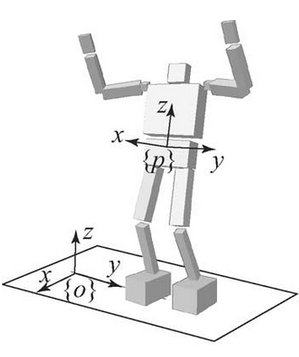
\includegraphics[width=0.4\textwidth]{chapter2/images/robot_component.png}
	\caption{ส่วนประกอบของหุ่นยนต์ฮิวมานอยด์}
	\label{fig:robot_component}
\end{figure}
หุ่นยนต์ฮิวมานอยด์ประกอบด้วยก้านต่อหลายๆก้านที่นำมาต่อกัน ลักษณะโครงสร้างนั้นจะเป็นแบบโซ่เปิด (Open kinematic chain)
และแต่ละก้านต่อจะเชื่อมต่อกันด้วยข้อต่อแบบหมุน เราสามารถแบ่งโครงสร้างของหุ่นยนต์ฮิวมานอยด์ออกเป็นส่วนหลักๆเป็น 2 ส่วน ส่วนแรกคือ
ส่วนก้านต่อของลำตัวหุ่นยนต์ (Torso) ซึ่งเราสามารถที่จะรวมไปถึงส่วนแขนกับหัวด้วย
และในส่วนที่สองคือ ส่วนก้านต่อของขาหุ่นยนต์ (Legs) ซึ่งเป็นส่วนขาของหุ่นยนต์ทั้งสองข้างที่สามารถนำไปที่สัมผัสกับพื้นได้
ทั้งสองก้านต่อนี้ถูกเชื่อมต่อกันด้วยส่วนของสะโพก (Hip) ที่อยู่ระหว่างส่วนลำตัวกับส่วนของขาหุ่นยนต์ ดังรูปที่ \ref{fig:robot_component}

\subsubsection{วัฏจักรการเดินของหุ่นยนต์ฮิวมานอยด์}
วัฏจักรการเดินของหุ่นยนต์ คือ การที่หุ่นยนต์จะต้องมีการถ่ายน้ำหนักไปมาระหว่างเท้าซ้ายและเท้าขวา
มีบางช่วงที่น้ำหนักตกลงบนเท้าข้างใดข้างหนึ่งหรือทั้งสองข้างพร้อมกัน สามารถแบ่งออกเป็นช่วงได้สองช่วง คือช่วงการยืนด้วยขาข้างเดียว
และช่วงการยืนด้วยขาทั้งสองข้าง
\begin{figure}[!ht]
	\centering
	\begin{subfigure}[b]{0.22\textwidth}
		\centering
		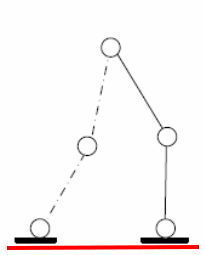
\includegraphics[width=\textwidth]{chapter2/images/doublesupport.png}
		\caption{ยืนด้วยขาสองข้าง}
		\label{fig:robot_walk_1}
	\end{subfigure}
	\hfill
	\begin{subfigure}[b]{0.45\textwidth}
		\centering
		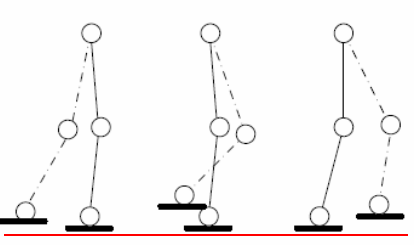
\includegraphics[width=\textwidth]{chapter2/images/singlesupport.png}
		\caption{ยืนด้วยขาข้างเดียว}
		\label{fig:robot_walk_2}
	\end{subfigure}
	\hfill
	\begin{subfigure}[b]{0.22\textwidth}
		\centering
		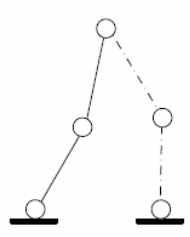
\includegraphics[width=\textwidth]{chapter2/images/doublesupport2.png}
		\caption{ยืนด้วยขาสองข้าง}
		\label{fig:robot_walk_3}
	\end{subfigure}
	\caption{วัฐจักรการเดินของหุ่นยนต์ฮิวมานอยด์}
	\label{fig:robot_walk_phase}
\end{figure}

\clearpage
\paragraph*{1) การยืนด้วยขาข้างเดียว :}
เป็นช่วงที่มีเท้าของหุ่นยนต์สัมผัสพื้นเพียงข้างเดียว ส่วนเท้าอีกข้างของหุ่นยนต์จะถูกยกลอยจากพื้น
โดยที่ไม่มีส่วนใดๆของขาข้างนั้นสัมผัสกับพื้นเลย ช่วงนี้จะเกิดขึ้นเมื่อมีการแกว่งเท้าจากข้างหลังไปข้างหน้า
ดังรูปที่ \ref{fig:robot_walk_2}

\paragraph*{2) การยืนด้วยขาสองข้าง :}
เป็นช่วงที่เท้าทั้งสองข้างของหุ่นยนต์สัมผัสกับพื้น ช่วงนี้จะเกิดตั้งแต่หุ่นยนต์วางเท้าขณะที่ส้นเท้าแตะกับพื้น
ไปจนถึง ปลายเท้าของขาอีกข้างหลุดออกจากพื้น

การเดินได้โดยไม่ล้มนั้น ตัวหุ่นยนต์จะต้องรักษาสมดุลของการเดินให้ได้ตลอดช่วงเวลาของการเดิน
ซึ่งสมดุลของการเดินแบบสองขาสามารถแบ่งตามลักษณะการเดินและการถ่ายน้ำหนักได้เป็น 2 รูปแบบหลัก คือ 
การเดินแบบสมดุลสถิต (static balance walking) และ การเดินแบบสมดุลพลวัต (dynamic balance walking)

\subsubsection{การสร้างและการควบคุมการเดินแบบสมดุลสถิต}
การเดินของหุ่นยนต์ในลักษณะนี้ จุดศูนย์กลางมวล (CoM) ของตัวหุ่นยนต์จะไม่มีการเคลื่อนไหวออกนอกบริเวณฐานรับน้ำหนัก (Supporting Area)
ตลอดช่วงเวลาการเดิน ไม่ว่าจะเป็นช่วงเวลาที่รับน้ำหนักด้วยเท้าข้างเดียวหรือทั้งสองข้างก็ตาม หมายความว่า โครงสร้างของหุ่นยนต์จะไม่ล้มแน่นอน
เนื่องจากการสร้างรูปแบบการเดินด้วยวิธีนี้จะควบคุมให้ตำแหน่งของจุดศูนย์กลางมวล อยู่ภายในพื้นที่ฐานรับน้ำหนักของหุ่นยนต์ตลอดเวลา
\ref{Legged robots walk the walk,https://blog.csiro.au/legged-robots-walk-walk/}

\begin{figure}[ht]
	\centering
	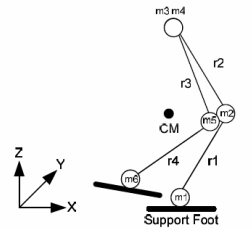
\includegraphics[width=0.4\textwidth]{chapter2/images/cominsupportpolygon.png}
	\caption{การควบคุมตำแหน่งของจุดรวมมวลให้อยู่ในพื้นที่ฐาน}
	\label{fig:robot_com_support}
\end{figure}

ข้อดีของการสร้างและควบคุมการเดินของหุ่นยนต์ด้วยวิธีนี้คือ สามารถสร้างรูปแบบการเดินได้โดยที่มีความซับซ้อนไม่มากนัก
สามารถสั่งให้หุ่นยนต์หยุดค้างในท่าทางใดๆก็ได้ตลอดเวลาโดยหุ่นยนต์ไม่ล้ม หุ่นยนต์ที่มีฝ่าเท้าใหญ่จะทำให้ง่ายต่อการก้าวเดินมากขึ้น
นอกจากการควบคุมการก้าวขาแล้วอาจเพิ่มการควบคุมส่วนลำตัวเพิ่มเติม เพื่อเป็นการเพิ่มเสถียรภาพในการเดินและการถ่ายเทน้ำหนัก
โดยที่อาจจะมีการเพิ่มเซนเซอร์วัดแรงที่ฝ่าเท้าเพื่อตรวจสอบการกระจายแรงกดที่ฝ่าเท้า เพื่อตรวจสอบว่าตำแหน่งของจุดรวมน้ำหนักอยู่บนพื้นที่ฝ่าเท้าหรือไม่
หรือเพื่อตรวจสอบเสถียรภาพของการเดินเพื่อแก้ไขท่าทางการเดินไม่ให้เกิดการล้ม

ข้อเสียของการควบคุมการเดินด้วยวิธีนี้คือ หุ่นยนต์จะใช้เวลาในการก้าวเดินมาก ใช้พลังงานในการเดินมากกว่าการเดินแบบสมดุลพลวัต
และท่าทางที่ได้จะมีความแตกต่างจากท่าทางการเดินของมนุษย์

\subsubsection{การสร้างและการควบคุมการเดินแบบสมดุลพลวัต}
การสร้างรูปแบบการเดินและควบคุมการเดินในลักษณะนี้ท่าทางการเดินของหุ่นยนต์นั้นจะคล้ายกับการเดินของมนุษย์มากกว่าแบบสถิต
เนื่องจากมีหลักการในการสร้างท่าทางที่เหมือนกับการเดินของมนุษย์ซึ่งมีขั้นตอนดังนี้คือ เอียงตัวให้ล้มไปในทิศทางที่ต้องการเดิน
เมื่อเริ่มเกิดการล้มขึ้นหุ่นยนต์จะเปลี่ยนตำแหน่งการวางเท้าไปยังตำแหน่งใหม่ เพื่อปรับให้โครงสร้างเข้าสู่สภาวะสมดุลอีกครั้ง

โดยธรรมชาติแล้วมนุษย์มีการถ่ายน้ำหนักในขณะที่เคลื่อนที่หรือยืนอยู่กับที่เพื่อรักษาสมดุลของท่าทางนั้นไว้
แต่หากการถ่ายโอนน้ำหนักนั้นเกิดสภาวะไม่สมดุล ร่างกายจะปรับสภาพโดยการเคลื่อนตำแหน่งของเท้าซึ่งเป็นพื้นที่ฐานออกจากเดิมไปยังตำแหน่งใหม่
เพื่อรักษาสมดุลไว้ หลักการดังกล่าวถูกนำมาใช้กับการควบคุมการเดินของหุ่นยนต์ฮิวมานอยด์ ในขณะที่หุ่นยนต์กำลังเคลื่อนไหว
ผลจากแรงเฉื่อยของการเคลื่อนที่และผลจากแรงดึงดูดของโลกมีผลต่อการเพิ่มและลดความเร่งให้การเดินของหุ่นยนต์
แรงเหล่านี้เรียกว่าแรงเฉื่อยรวมของการเคลื่อนที่ และเมื่อเท้าหุ่นยนต์สัมผัสกับพื้นจะได้รับผลกระทบของแรงนี้ เรียกว่า
แรงปฏิกิริยาจากพื้น

การตัดกันระหว่างแรงปฏิกิริยาจากพื้นและแนวแรงเฉื่อยรวม ตำแหน่งนั้นหากทำให้โมเมนต์เท่ากับศูนย์
เรียกจุดตัดนี้ว่าจุดโมเมนต์ศูนย์ ($ZMP_{robot}$) และจุดที่แรงปฏิกิริยาลงสู่พื้นว่า จุดปฏิกิริยาพื้นฐาน 
ท่าทางการเดินของหุ่นยนต์จะถูกกำหนดและถูกส่งให้กับชุดควบคุมข้อต่อจุดต่างๆของหุ่นยนต์ โดยให้สอดคล้องกับแรงเฉื่อยรวมที่เกิดขึ้นจากการคำนวณ
เรียกว่าแรงเฉื่อยรวมเป้าหมาย และจุดโมเมนต์ศูนย์ที่ได้จากการคำนวณเรียกว่าจุดโมเมนต์ศูนย์เป้าหมาย ($ZMP_{target}$)
เมื่อหุ่นยนต์เกิดสมดุลในขณะที่ทำการเดินได้อย่างสมบูรณ์ แนวแกนของแรงเฉื่อยรวมเป้าหมายและแรงปฏิกิริยาที่พื้นจะเป็นตำแหน่งเดียวกัน
แต่ในขณะที่หุ่นยนต์เดินผ่านพื้นผิวที่มีความขรุขระหรือไม่เรียบตำแหน่งสองจุดดังกล่าง จะไม่ใช่ตำแหน่งเดียวกันทำให้หุ่นยนต์เกิดการล้มได้
แรงที่ทำให้เกิดการล้มนี้เกิดจากตำแหน่งของจุดโมเมนต์ศูนย์และตำแหน่งแรงปฏิกิริยารวมที่พื้นไม่ตรงกัน ซึ่งเป็นสาเหตุหลักที่ทำให้เกิดความไม่สมดุลขึ้น
และเมื่อหุ่นยนต์เสียสมดุลระบบที่จะสามารถป้องกันการล้มและทำให้หุ่นยนต์เดินต่อไปได้อย่างต่อเนื่องคือ ระบบควบคุมแรงปฏิกิริยา
ระบบควบคุมจุดโมเมนต์ศูนย์ และระบบควบคุมการวางเท้า\ref{Achieving Stable walking,http://world.honda.com/ASIMO/history/technology2.html}

\begin{figure}[!ht]
	\centering
	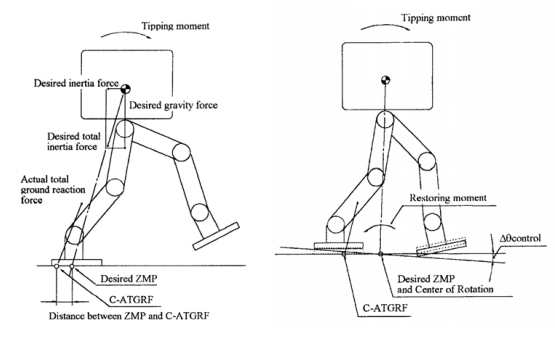
\includegraphics[width=0.7\textwidth]{chapter2/images/zmpdynamicwalking.png}
	\caption{การควบคุมตำแหน่งของจุดโมเมนต์ศูนย์ให้ตรงกับแรงปฏิกิริยารวม}
	\label{fig:robot_zmp_support}
\end{figure}

อย่างไรก็ตาม การสร้างท่าทางการเดินในลักษณะนี้ต้องใช้สมการในการคำนวณที่ซับซ้อนมาก
เนื่องจากต้องหาความสัมพันธ์ระหว่างองค์ประกอบหลายส่วน เช่น น้ำหนักของโครงสร้างในแต่ละส่วน 
แรงบิดที่แต่ละข้อต่อ และโมเมนต์โดยรวมของระบบ นอกจากนี้ยังต้องใช้อุปกรณ์การตรวจวัดต่างๆ เช่น เซนเซอร์วัดแรง
เซนเซอร์วัดมุม เซนเซอร์วัดแรงบิด ติดตั้งตามจุดต่างๆของโครงสร้างเพื่อวัดค่าออกมา ก่อนที่จะทำการคำนวณตำแหน่ง
และสร้างท่าทางการเดินของหุ่นยนต์ฮิวมานอยด์ ท่าทางการเดินที่ได้จากการควบคุมด้วยวิธีนี้ จะมีความคล้ายคลึงกับท่าทางการเดินของมนุษย์มาก

\subsubsection{จุดศูนย์กลางมวลของหุ่นยนต์}
หากต้องการให้หุ่นยนต์สามารถที่จะทรงตัวอยู่ได้โดยไม่ล้มนั้น จึงต้องรู้ตำแหน่งจุดศูนย์กลางมวลของหุ่นยนต์ตลอดเวลา
และต้องให้จุดศูนย์กลางมวลฉายตกในบริเวณฐานรับน้ำหนักของหุ่นยนต์โดยหาจากพื้นที่ที่ฝ่าเท้าสัมผัสกับพื้น
วิธีการนี้เป็นวิธีการทางสถิตศาสตร์

\clearpage
\section{งานวิจัยที่เกี่ยวข้อง}
\subsection{ตัวอย่างหุ่นยนต์ฮิวมานอยด์}
\subsection*{Poppy Humanoid}
\begin{figure}[htbp]
    \centering
    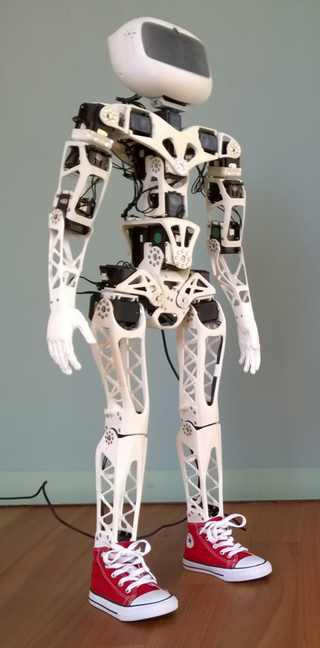
\includegraphics[width=0.3\textwidth]{chapter2/images/PoppyHumanoid1.png}
    \caption{หุ่นยนต์ฮิวมานอยด์ป๊อปปี้}
    \label{fig:poppy_humanoid}
\end{figure}
หุ่นยนต์ฮิวมานอยด์ป๊อปปี้ ถูกสร้างขึ้นมาเพื่อใช้ในงานศิลปะ การวิจัยและการศึกษาโดยเฉพาะ 
หุ่นยนต์ป๊อปปี้ประกอบด้วยส่วนของฮาร์ทแวร์และซอฟแวร์ที่เปิดเป็นโอเพนซอร์ซให้ผู้ที่สนใจสามารถเข้ามาศึกษาได้
โปรแกรมของหุ่นยนต์ใช้โมดูลที่มีชื่อว่า Pypot ที่เป็นส่วนเสริมของภาษา Python ในการพัฒนาซอฟแวร์
ทุกคนสามารถเข้าถึงข้อมูลเชิงเทคนิคของหุ่นยนต์ฮิวมานอยด์ป๊อปปี้ได้ เช่น ส่วนรายละเอียดการทำงาน
คลิปวีดีโอสอนการประกอบ การใช้ระบบจำลอง และการพัฒนาต่างๆผ่านทางเว็บไซต์ http://www.poppy-project.org 
หุ่นยนต์ป๊อปปี้มีส่วนของโครงสร้างที่ผลิตมาจากพลาสติด PLA และ ABS โดยใช้เทคนิคการขึ้นรูปด้วยเครื่องพิมพ์สามมิติ
ตัวขับเคลื่อนข้อต่อต่างๆใช้เป็น Dynamixel Digital Servo และควบคุมคำสั่งของตัวขับเคลื่อนด้วย 
คอมพิวเตอร์ขนาดเล็ก Odroid UX4 ใช้ระบบปฎิบัติการ Ubuntu 14.04 
ตัวของหุ่นยนต์มีความสูง 83 เซนติเมตร น้ำหนัก 3.5 กิโลกรัม 
ใช้เซนเซอร์วัดมุมเอียงเป็น IMU ที่มีองศาอิสระเท่ากับ 9 องศาอิสระ ในการควบคุมเสถียรภาพในการเดินของตัวเอง
มีองศาอิสระหรือจำนวนตัวขับเคลื่อนทั้งหมด 25 องศา ประกอบไปด้วย ขาข้างละ 6 องศาอิสระ แขนข้างละ 4 องศาอิสระ 
ลำตัว 3 องศาอิสระ และ หัว 2 องสาอิสระ

\clearpage
\subsection*{iCub Humanoid}
\begin{figure}[htbp]
    \centering
    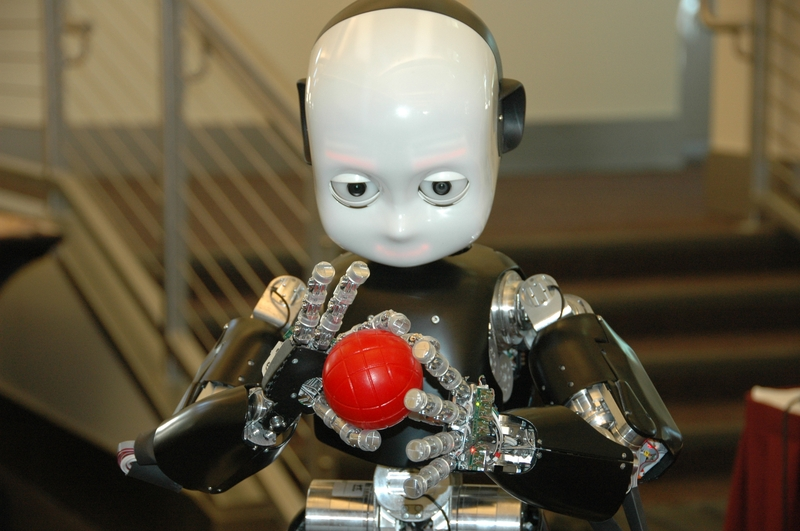
\includegraphics[width=0.6\textwidth]{chapter2/images/icub-1.jpg}
    \caption{หุ่นยนต์ฮิวมานอยด์ไอคัพ}
    \label{fig:icub_humanoid}
\end{figure}
หุ่นยนต์ฮิวมานอยด์ไอคัพ ถูกออกแบบโดยมหาวิทยาลัยหลายแห่งในยุโรปรวมกลุ่มกันขึ้นมาในชื่อ RobotCub
และถูกสร้างขึ้นโดย Istituto Italiano di Tecnologia (IIT) ตัวหุ่นยนต์ไอคัพนั้นมีความสูงอยู่ที่ 1 เมตร
น้ำหนักโดยรวมทั้งหมดประมาณ 22 กิโลกรัม วัสดุที่ใช้ในการสร้างแตกต่างกันไปในแต่ละส่วนของร่างกายโดยจะใช้
aluminum alloy AI6082 สำหรับส่วนที่ต้องรับภาระความเครียดน้อย ใช้ aluminum alloy 7075(Ergal) สำหรับส่วนที่ต้องรับภาระความเครียดปานกลางถึงสูง
และใช้ Stainless Steel 17-4PH ในส่วนของเพลาข้อต่อต่างๆเพื่อให้มีความแข็งแรงสูง ตัวหุ่นยนต์ถูกออกแบบให้มีลักษณะเหมือนเด็กอายุ 3-4 ขวบ
ควบคุมโดยใช้บอร์ดไมโครคอนโทรเลอร์เป็นรุ่น PC104 Controller ภาษาที่ใช้ในการพัฒนาใช้เป็นภาษา C++ ในการเขียนโปรแรม
การติดต่อสื่อสารกับตัวขับเคลื่อนหรือมอเตอร์ตามข้อต่อต่างๆ และเซนเซอร์ ผ่านทางโปรโตคอล CAN Bus เพื่อทำให้ใช้สายน้อยลง
ใช้เส้นเอ็นในการส่งถ่ายแรงขับเคลื่อนไปยังส่วนของข้อต่อส่วนมือและไหล่ นิ้วของหุ่นยนต์ถูกร้อยด้วย สายเคเบิลเคลือบ Teflon อยู่ภายใน
และคลายตัวกลับสู่สภาวะสมดุลได้ด้วยแรงของสปริง เซนเซอร์วัดมุมของข้อต่อแต่ละตัวใช้การออกแบบให้มี Hall-effect ติดอยู่
ช่วยในการอ่านค่าของตำแหน่งและความเร็วที่เกิดขึ้นที่ข้อต่อนั้น หุ่นยนต์ไอคัพมีองศาอิสระรวมกันทั้งหมด 53 องศาอิสระ
ประกอบไปด้วย แขนข้างละ 7 องศาอิสระ มือข้างละ 9 องศาอิสระ หัว 6 องศาอิสระ ลำตัว 3 องศาอิสระ และขาข้างละ 6 องศาอิสระ
ในส่วนของหัวจะประกอบไปด้วย กล้องสองตัวเพื่อทำสเตอริโอวิชั่น ไมโครโฟนสำหรับรับเสียงจากสภาพแวดล้อมภายนอก
และไฟแสดงอารมณ์บริเวณปากและคิ้ว หุ่นยนต์นี้ไม่ได้ถูกออกแบบให้มีการทำงานเป็นแบบอัตโนมัติ ซึ่งก็คือตัวหุ่นยนต์นั้นไม่มีแบตเตอรี่ภายในตัว
แต่ใช้แหล่งพลังงานจากภายนอกโดยการส่งเข้าไปผ่านสายเคเบิล และเชื่อมต่อกับอินเทอร์เน็ตผ่านสายแลน (LAN)

\clearpage
\subsection*{Darwin-OP Humanoid}
\begin{figure}[htbp]
    \centering
    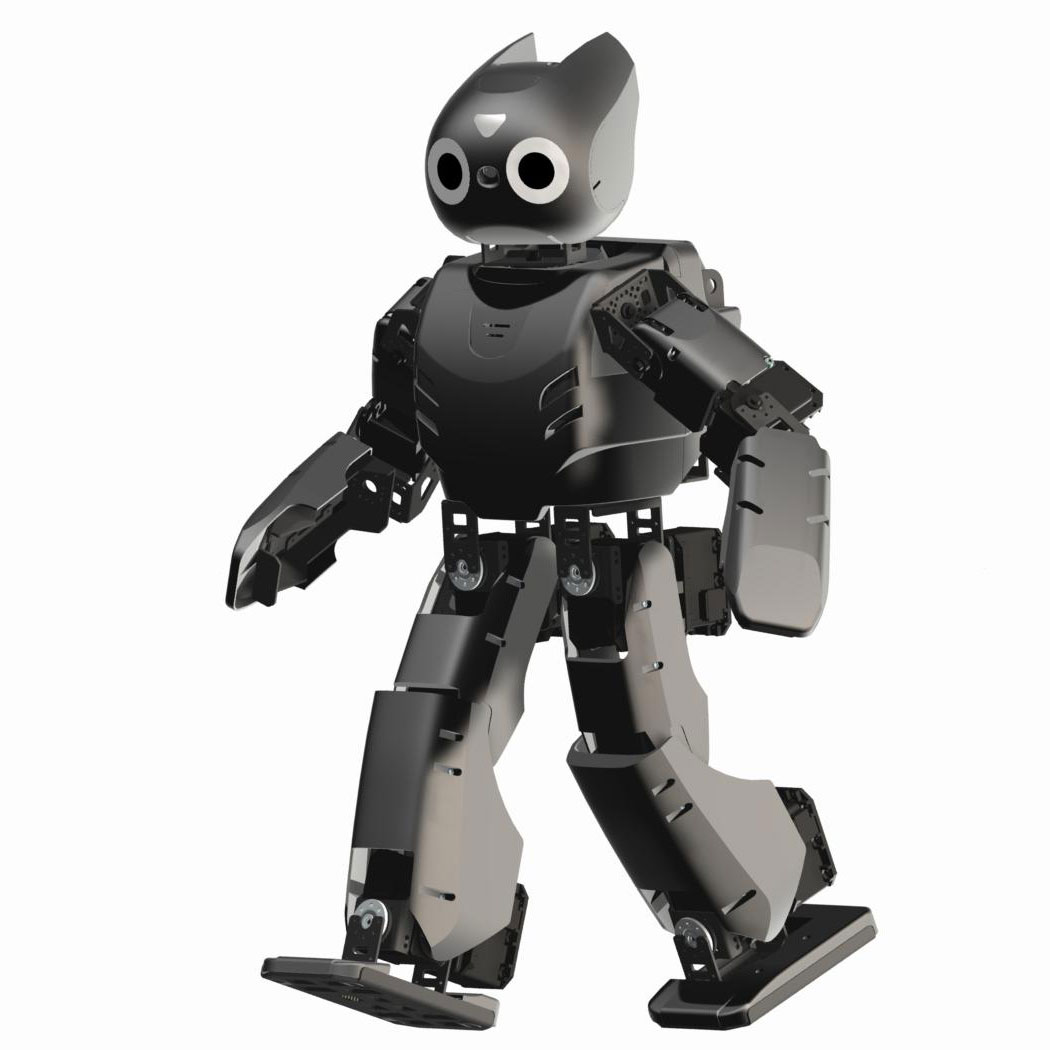
\includegraphics[width=0.55\textwidth]{chapter2/images/Darwin_OP_6.jpg}
    \caption{หุ่นยนต์ฮิวมานอยด์ดาร์วิน}
    \label{fig:darwin_humanoid}
\end{figure}
หุ่นยนต์ฮิวมานอยด์ดาร์วิน (Darwin-OP) เป็นชื่อที่ย่อมาจากคำว่า Dynamic Anthropomorphic Robot
with Intelligence–Open Platform
เป็น OpenSource Platform ที่ถูกออกแบบและพัฒนาโดย Korean robot manufacturer Robotis
โดยมีความร่วมมือกับ Virginia polytechnic institude and state university, Purdue university และ University of Pennsylvania
หุ่นยนต์ฮิวมานอยด์ดาร์วินมีความสามารถในการรับภาระโหลดได้สูง เนื่องจากมีการพัฒนามอเตอร์เป็นของตัวเอง อีกทั้งยังมีความสามารถในการเคลื่อนที่แบบ
พลวัต (Dynamic) หุ่นยนต์ดาร์วิน มีองศาอิสระทั้งหมด 20 องศาอิสระ ซึ่งประกอบไปด้วย ขาข้างละ 6 องศาอิสระ แขนข้างละ 3 องศาอิสระ และหัว 2 องศาอิสระ
ขับเคลื่อนข้อต่อต่างๆด้วยเซอร์โวมอเตอร์ Dynamixel MX-28T ที่มีการเชื่อมต่อแบบ RS485 ในการประหยัดสายที่ใช้ในการสั่งการ มอเตอร์แต่ละตัวมีเซนเซอร์วัดตำแหน่ง 
และความเร็วอยู่ภายใน ตัวหุ่นยนต์มีความสูงทั้งหมด 45 เซนติเมตร มีน้ำหนักโดยประมาณ 2.9 กิโลกรัม
ระบบภายในใช้คอมพิวเตอร์ขนาดเล็กเป็น 1.6 GHz Intel Atom Z530 (32 bit) ใช้คอนโทรเลอร์ ARM CortexM3 STM32F103RE 72 MHz 
และมีเซนเซอร์วัดมุมเอียงเป็น 3-axis gyro, 3-axis accelerometer เพื่อช่วยในการควบคุมเสถียรภาพในการเดิน

\clearpage
\subsection*{Nao Humanoid}
\begin{figure}[htbp]
    \centering
    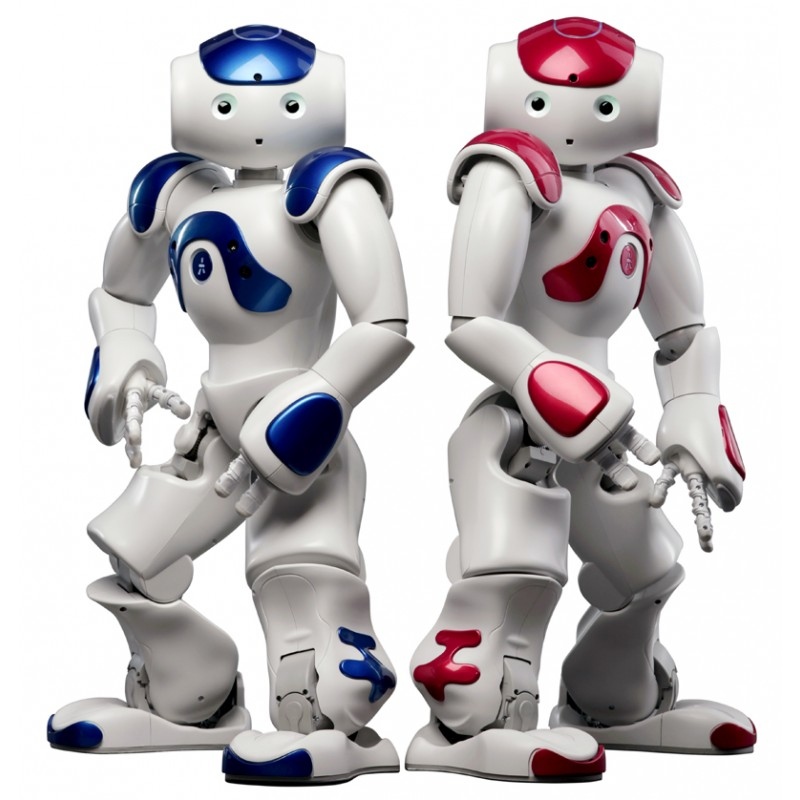
\includegraphics[width=0.55\textwidth]{chapter2/images/nao.jpg}
    \caption{หุ่นยนต์ฮิวมานอยด์นาโอะ}
    \label{fig:nao_humanoid}
\end{figure}
หุ่นยนต์ฮิวมานอยด์นาโอะ เป็นหุ่นยนต์ฮิวมานอยด์ขนาดกลาง ถูกผลิตมาจากประเทศฝรั่งเศษ พัฒนาโดยบริษัท Aldebaran Robotics เมื่อปี 2004 และในปี 2007
หุ่นยนต์ฮิวมานอยด์นาโอะได้นำไปแทนที่หุ่นยนต์สุนัขของ Sony ชื่อ Aibo ขณะถูกใช้ในรายการแข่งขัน RoboCup Standard Platform League (SPL) หุ่นยนต์นาโอะได้ถูกนำไปใช้ใน Robocup 2008 และ 2009 
หุ่นยนต์นาโอะถูกพัฒนาออกมาหลายรุ่นมีองศาอิสระตั้งแต่ 14 องศาอิสระ 21 องศาอิสระ และ 25 องศาอิสระ สำหรับเพื่องานวิจัยนั้นมีถึง 25 องศาอิสระ
โดยเพิ่มเติมมือสองข้างเอาเข้าไปเพื่อให้สามารถหยิบจับสิ่งของได้ ภายในหุ่นยนต์ถูกควบคุมด้วยระบบปฎิบัติการ NAO 2.0 (Linux-based) ตัวหุ่นยนต์มีความสูง 58 เซนติเมตร 
น้ำหนัก 4.3 กิโลกรัม ส่วนเซนเซอร์การรับรู้ต่างๆจะประกอบไปด้วย เซนเซอร์วัดมุมเอียง 3-axis gyro, 3-axis accelerometer, Ultrasound captors, ไมโครโฟน 4 ตัว ลำโพง 2 ตัว กล้อง 2 ตัว เพื่อใช้ประโยชน์ในการทำงานวิจัยต่างๆ
ตอนนี้ความสามารถของหุ่นยนต์นาโอะที่ทำได้คือ สามารถเทน้ำส้มได้ เดินขึ้นลงบันไดและทางลาดชันได้ ระหว่างการเดินนั้นสามารถวางแผนการวางเท้าได้อย่างรวดเร็ว
อีกทั้งยังสามารถที่จะเดินหลบหลีกสิ่งกีดขวางได้ด้วย

\clearpage
\subsection*{Wabot}
\begin{figure}[htbp]
    \centering
    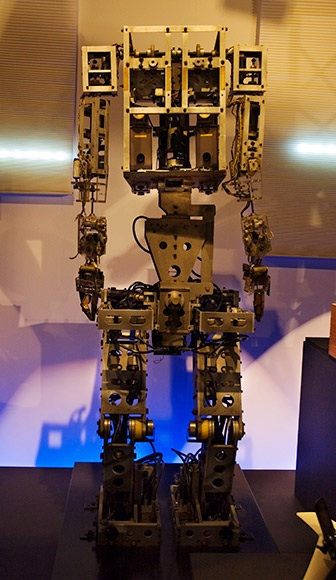
\includegraphics[width=0.45\textwidth]{chapter2/images/wabot.jpg}
    \caption{หุ่นยนต์ฮิวมานอยด์วาบอท}
    \label{fig:wabot_humanoid}
\end{figure}
หุ่นยนต์ฮิวมานอยด์มีการพัฒนาในช่วงแรกเริ่มมาตั้งแต่ปี 1973 หุ่นยนต์ฮิวมานอยด์ ตัวแรกชื่อ Wabot-1 เริ่มสร้างโดยมหาวิทยาลัย Waseda ที่ประเทศญี่ปุ่น ตัวของหุ่นยนต์มีความสูง 180 เซนติเมตร
น้ำหนัก 210 กิโลกรัม โดยหุ่นยนต์สามารถติดต่อสื่อสารกับมนุษย์ได้ด้วยภาษาญี่ปุ่น สามารถวัดระยะและทิศทางได้โดยใช้การรับรู้ผ่านทางตาและหูเทียม หุ่นยนต์ Wabot-1 นั้นสามารถเดินได้ด้วยขาของตนเองที่มีสองข้าง
สามารถหยิบและเคลื่อนย้ายวัตถุด้วยมือ ต่อมาในปี 1984 มหาวิทยาลัย Waseda ได้พัฒนาหุ่นยนต์ฮิวมานอยด์ที่ชื่อ Wabot-2 โดยหุ่นยนต์สามารถสื่อสารกับมนุษย์ได้ สามารถอ่านโน๊ตเพลงและเล่นดนตรีโดยใช้ electronic organ แบบง่ายๆได้
และในปี 1985 บริษัท Hitachi ได้สร้างหุ่นยนต์ WHL-11 ที่มีสองขาเหมือนมนุษย์ ซึ่งสามารถเดินแบบสมดุลสถิต (Static Walking) บนพื้นราบได้ด้วยความเร็ว 13 วินาทีต่อหนึ่งก้าว และสามารถเลี้ยวได้ซ้ายและขวาได้


\clearpage
\subsection{งานวิจัยการออกแบบระบบหุ่นยนต์ฮิวมานอยด์}






\clearpage
\section{การออกแบบโครงสร้างของหุ่นยนต์}
\subsection{ความแตกต่างระหว่างโครงสร้างของมนุษย์กับโครงสร้างของหุ่นยนต์}

\subsubsection{ความแตกต่างขององศาเสรี}
เนื่องจากลักษณะข้อต่อของมนุษย์มีความซับซ้อนมากกว่าโครงสร้างของหุ่นยนต์
ทำให้ข้อต่อแต่ละจุดของมนุษย์นั้นสามารถหมุนได้หลายทิศทาง รวมถึงขอบเขตของการหมุนของข้อต่อในแต่จุดก็มีความแตกต่างกัน
ในการนำรูปแบบการเดินของมนุษย์ไปใช้กับหุ่นยนต์จึงต้องปรับค่ามุมที่ข้อต่อให้มีความเหมาะสมกับโครงสร้าง
และข้อจำกัดเกี่ยวกับการหมุนของข้อต่อจุดต่างๆของหุ่นยนต์ที่จะใช้ทดสอบด้วย

\subsubsection{ความแตกต่างของอัตราส่วน}
นอกจากความแตกต่างขององศาเสรี (DoF) ระหว่างมนุษย์กับหุ่นยนต์แล้ว
ความแตกต่างของอัตราส่วนระหว่างโครงสร้างแต่ละส่วนของมนุษย์กับหุ่นยนต์เป็นอีกสาเหตุหนึ่ง
ที่ต้องทำการปรับแต่งใหม่มีความเหมาะสม เนื่องจากความยาวของโครงสร้างแต่ละส่วน
รวมทั้งระยะห่างระหว่างจุดหมุนแต่ละจุดของมนุษย์กับหุ่นยนต์ที่มีความแตกต่างกัน
ดังนั้นจึงต้องกำหนดระบบพิกัดสำหรับหุ่นยนต์ฮิวมานอยด์ขึ้นมาใหม่ เพื่อใช้ในการอ้างอิงจุดหมุน
และความยาวของโครงสร้างในส่วนต่างๆ
\begin{figure}[htbp]
    \centering
    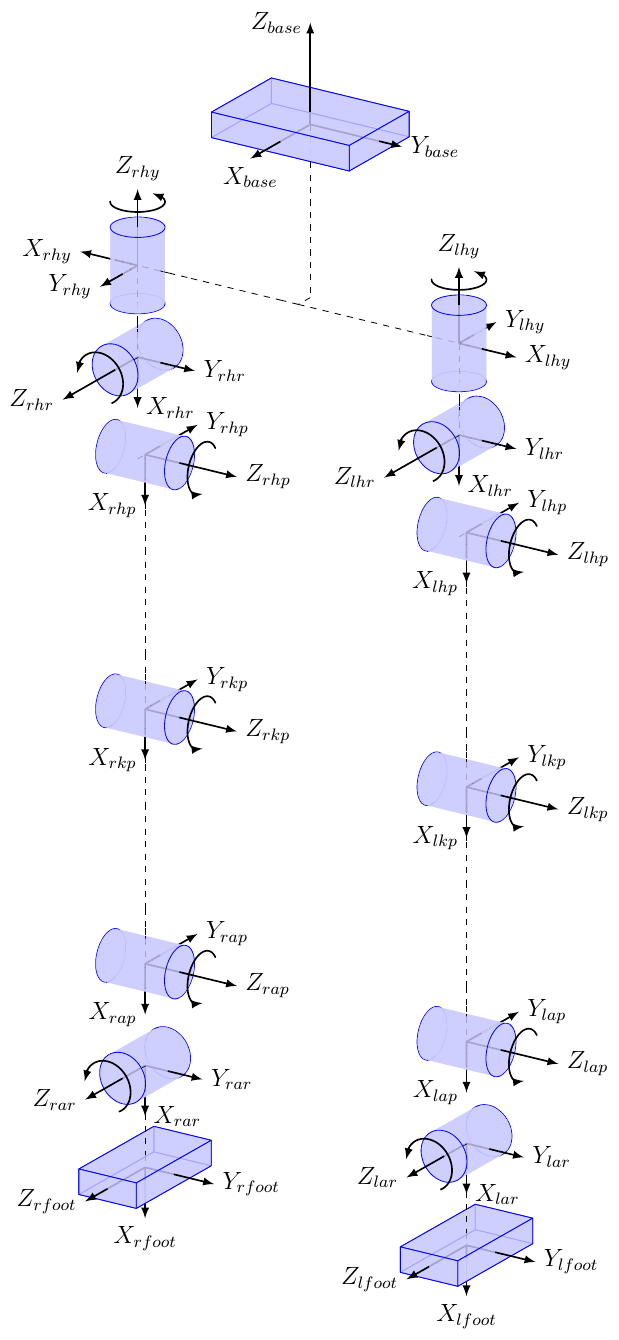
\includegraphics[width=0.40\textwidth]{chapter2/images/uthai_kinematics.png}
    \caption{ตัวอย่างตำแหน่งและการหมุนของข้อต่อของหุ่นยนต์เพื่อการอ้างอิง}
    \label{fig:robot_frame}
\end{figure}

\subsubsection{กำลังและประสิทธิภาพของมอเตอร์}
ความสามารถในการรับน้ำหนักของข้อต่อแต่ละจุดมีความแตกต่างกัน การเคลื่อนไหวของมนุษย์นั้นจะมีกล้ามเนื้อ
และเส้นเอ็นเป็นตัวออกแรงดึงส่วนต่างๆของร่างกายเพื่อทำให้เกิดการเคลื่อนไหวซึ่งจะมีความยืดหยุ่นและแรงดึงที่มีค่าสูง
สำหรับการเคลื่อนไหวของหุ่นยนต์ จะใช้การบิดแกนของเซอร์โวมอเตอร์ (Servo Motor) หรือมอเตอร์ที่ติดอยู่ที่ข้อต่อจุดต่างๆ
ทำให้ความสามารถในการรับน้ำหนัก แรงบิดและความยืดหยุ่นที่ข้อต่อขึ้นกับกำลังของมอเตอร์เป็นหลัก
การสร้างท่าทางของหุ่นยนต์จึงต้องคำนึงถึงความสามารถในการรับน้ำหนักและกำลังของเซอร์โวมอเตอร์ที่ใช้ด้วยเช่นกัน

%%%%%%%%%%%%%%%%%%%%%%%%%%%%%%%%%%%%%%%%%%%%%%%%%%%%%%%%%
\subsection{วัสดุและการขึ้นรูปโครงสร้างของหุ่นยนต์ฮิวมานอยด์}
\begin{figure}[htbp]
    \centering
    
\includegraphics[width=0.40\textwidth]{chapter2/images/toedit.jpg}
    \caption{รอแก้ไข}
    \label{fig:toedit}
\end{figure}

%%%%%%%%%%%%%%%%%%%%%%%%%%%%%%%%%%%%%%%%%%%%%%%%%%%%%%%%%
\subsection{อุปกรณ์ที่ใช้ในหุ่นยนต์ฮิวมานอยด์}

\subsubsection{ระบบจ่ายพลังงาน}
\subsubsection{ตัวขับเคลื่อน}

\subsubsection{หน่วยประมวลผลควบคุม}
ในการควบคุมหุ่นยนต์ฮิวมานอยด์ให้สามารถทำกิจกรรมต่างๆได้นั้น ส่วนที่มีความสำคัญที่ขาดไปไม่ได้ คือ
หน่วยประมวลผลระบบควบคุม ถ้าหากไม่มีระบบประมวลผลควบคุมแล้ว อุปกรณ์ต่างๆ ที่ติดตั้งอยู่ภายในตัวของหุ่นยนต์ฮิวมานอยด์จะไม่สามารถติดต่อสื่อสารกันได้
ซอฟท์แวร์ของหุ่นยนต์ที่พัฒนามาทั้งหมดจะไม่สามารถใช้ได้ ทำให้หุ่นยนต์ฮิวมานอยด์ไม่สามารถทำงานในสิ่งที่ต้องการได้ 
การวางแผนระบบควบคุมที่นิยมใช้ในระบบหุ่นยนต์ฮิวมานอยด์ส่วนใหญ่ จะแบ่งออกเป็น 2 ส่วนด้วยกัน 
คือส่วนของหน่วยประมวลผลควบคุมระดับสูง และหน่วยประมวลผลควบคุมระดับต่ำ

\subsubsection*{หน่วยประมวลผลควบคุมระดับสูง (High level controller)}
หน่วยประมวลผลควบคุมระดับสูงเป็นส่วนที่ใช้ประมวลผลการทำงานที่มีความซับซ้อนของระบบเช่น
จลนศาสตร์ของหุ่นยนต์ การคำนวณหาเส้นทางการเดิน ในการคำนวณทางคณิตศาสตร์ของระบบเหล่านี้จำเป็นต้องมีการประมวลผลที่เร็ว
และมีประสิทธิภาพ ย้อนไปในสมัยที่มีการพัฒนาหุ่นยนต์ฮิวมานอยด์ยุคแรกเริ่มนั้น หน่วยประมวลผลควบคุมระดับสูง
จะใช้คอมพิวเตอร์เป็นตัวในการประมวลผลการคำนวณ ซึ่งคอมพิวเตอร์สมัยนั้นมีขนาดใหญ่ น้ำหนักมาก
และต้องใช้หลังงานสูง ซึ่งต่างจากปัจจุบันนี้ที่มีการพัฒนาของเทคโนโลยีที่ก้าวหน้ามากขึ้น
ทำให้คอมพิวเตอร์มีขนาดเล็กลงเทียบเท่ากับบอร์ดคอนโทรเลอร์ทั่วไป ในที่นี้จะทำการยกตัวอย่างของบอร์ดคอมพิวเตอร์ที่มีวางจำหน่ายในปัจจุบัน
และทำการรวมรวมเทียบเคียงประสิทธิภาพ ของบอร์ดคอมพิวเตอร์แต่ละชนิดไว้ดังนี้
\begin{figure}[htbp]
    \centering
    
\includegraphics[width=0.40\textwidth]{chapter2/images/toedit.jpg}
    \caption{รอแก้ไข}
    \label{fig:toedit}
\end{figure}

\subsubsection*{หน่วยประมวลผลควบคุมระดับต่ำ (Low level controller)}
หน่วยประมวลผลควบคุมระดับต่ำเป็นส่วนที่รับคำสั่งบางอย่างมาจาก หน่วยประมวลผลควบคุมระดับสูง
มีประสิทธิภาพในการประมวลผลการคำนวณที่น้อยกว่า เนื่องจากการออกแบบสถาปัตยกรรมภายในระบบไม่เอื้ออำนวยต่อการคำนวณที่มีความซับซ้อน
แต่มีความสามารถในการประมวลผลระบบที่เป็นคาบได้อย่างแม่นยำ ในด้านการทำหุ่นยนต์ฮิวมานอยด์นั้นมักจะใช้หน่วยประมวลผลควบคุมระดับต่ำ
ในการติดต่อกับอุปกรณ์ต่าง ๆบนตัวของหุ่นยนต์ฮิวมานอยด์โดยตรง เช่น ตัวขับเคลื่อน เซนเซอร์รับค่า หรือไฟแสดงสถานะต่างๆของหุ่นยนต์
\begin{figure}[htbp]
    \centering
    
\includegraphics[width=0.40\textwidth]{chapter2/images/toedit.jpg}
    \caption{รอแก้ไข}
    \label{fig:toedit}
\end{figure}
จากตารางข้างต้นเป็นตารางเปรียบเทียบประสิทธิภาพและความเหมาะสมกับการใช้งาน จะเห็นได้ว่า Nucleo
มีประสิทธิภาพมากกว่าในหลายๆด้านไม่ว่าจะเป็น Core Clock ที่เร็วถึง 100 MHz หรือ GPIO ที่มีมาให้ 50
ช่องการเชื่อมต่อ อีกทั้งยังมี I2C ซึ่งเป็นรูปแบบที่ใช้ในการติดต่อกับ IMU ที่ต้องใช้ ทั้งนี้ ทั้ง 2
รุ่นที่ได้ทำการเปรียบเทียบนี้ไม่รองรับ RS – 485 โดยตรง ซึ่งเป็นรูปแบบการสื่อสารที่จะใช้กับการติดต่อกับตัวขับเคลื่อน
%ฉะนั้นแล้วทางผู้วิจัยจึงเลือกที่จะใช้ Nucleo แล้วมีการใช้โมดูลการสื่อสาร UART to RS-485 เพิ่มเติม

\subsubsection{เซนเซอร์ตรวจหน้าสัมผัสที่พื้น}
เซนเซอร์ตรวจหน้าสัมผัสที่พื้นเป็นเซนเซอร์ที่ถูกติดตั้งบริเวณฝ่าเท้า เพื่อตรวจสอบการเดินของหุ่นยนต์ฮิวมานอยด์ว่าขณะนี้มีการสัมผัสของฝ่าเท้าของหุ่นยนต์กับพื้นหรือไม่
ซึ่งในงานวิจัยนี้ได้ใช้หลักการตัวตรวจจับแรงกดแบบค่าความต้านทานหรือ Force Sensing Resistor (FSR) ที่ใช้เทคโนโลยีฟิล์มโพลีเมอร์แบบหนาโดยที่
เซนเซอร์สามารถเปลี่ยนแรงที่มากระทำให้อยู่ในรูปของการเปลี่ยนแปลงค่าความต้านทานไฟฟ้า ตัวเซนเซอร์มีลักษณะเป็นแผ่น มีโครงสร้าง 5 ชั้น
โดยสองชั้นนอกสุดเป็นฟิล์มของโพลีเอสเตอร์ สองชั้นถัดเข้ามาเป็นฟิล์มของโลหะที่เป็นตัวนำไฟฟ้า และชั้นในสุดเป็นหมึกที่มีความไวในการตอบสนองต่อแรงภายนอกที่มากระทำ
(Pressure sensitive ink) และโครงสร้างทั้ง 5 ชั้น ถูกรวมเข้าด้วยกันด้วยวิธีลามิเนท จึงทำให้เซนเซอร์วัดแรงนี้มีลักษณะแบนมีความยืดหยุ่นสูง
ด้วยเหตุนี้จึงทำให้เซนเซอร์สามารถโค้งงอได้ง่าย แรงดันไฟฟ้าที่ตกคร่อมตัวตรวจจับจะลดลง เมื่อมีแรงกดมากระทำบนแผ่นตรวจจับ มีโครงสร้างของตัวตรวจจับแสดงในรูปที่ \ref{fig:fsr_sensor} 

\begin{figure}[htbp]
    \centering
    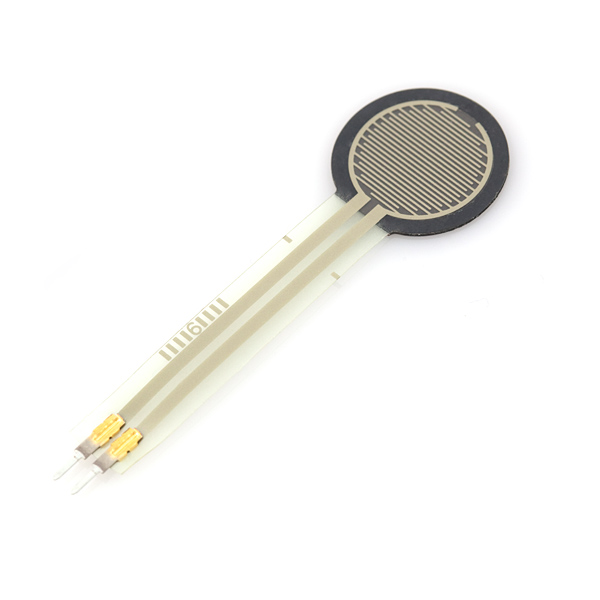
\includegraphics[width=0.25\textwidth]{chapter2/images/FSRx.jpg}
    \caption{ลักษณะโครงสร้างของตัวตรวจจับแรงกด FSR}
    \label{fig:fsr_sensor}
\end{figure}

\begin{figure}[htbp]
    \centering
    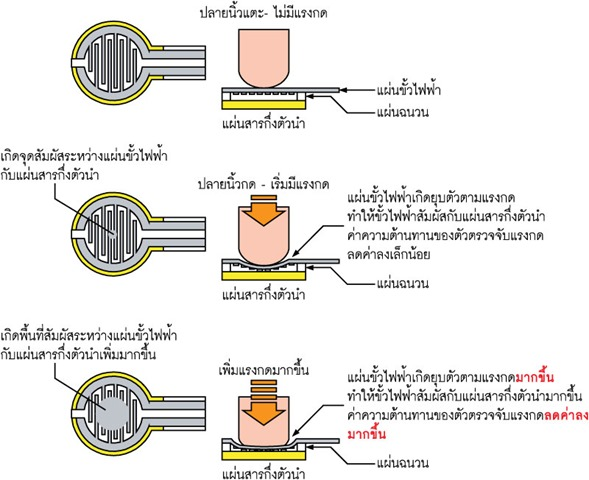
\includegraphics[width=0.65\textwidth]{chapter2/images/FSR.jpg}
    \caption{การทำงานของตัวตรวจจับแรงกด FSR}
    \label{fig:fsr_sensor_2}
\end{figure}

\subsubsection{เซนเซอร์วัดความเฉื่อย}

\begin{figure}[htbp]
    \centering
    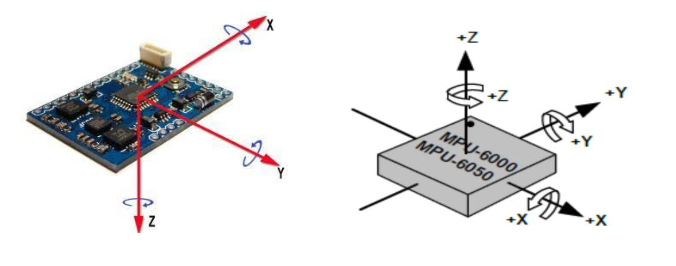
\includegraphics[width=0.65\textwidth]{chapter2/images/imu.png}
    \caption{เซนเซอร์วัดความเฉื่อย}
    \label{fig:imu_sensor}
\end{figure}

Inertial Measurement Unit (IMU) เป็นส่วนประกอบหลักที่ใช่ในการนำร่องเครื่องบิน ยาน-อวกาศ ดาวเทียม เรือ
ขีปนาวุธ ซึ่งในตัวของ IMU ประกอบไปด้วยสองส่วนหลักคือ Accelerometers 3 ทิศทาง ในการรับความเร่งเชิงเส้น
และ Gyroscopes 3 ทิศทาง ในการบอกความเร็วเชิงมุม เซนเซอร์ตัวนี้สามารถนำมาใช้ในการหาทิศทางการหมุนของตัวหุ่นยนต์ฮิวมานอยด์ได้

เซนเซอร์วัดความเร็ว (Gyroscope) เป็นอุปกรณ์สำหรับการวัดความเร็ว หรือการรักษาการปรับทิศทาง ขึ้นอยู่กับหลักการของการอนุรักษ์โมเมนตัมเชิงมุม
ถ้าไม่มีการเคลื่อนที่ อัตราการเปลี่ยนแปลงมุมจะมีค่าเท่ากับศูนย์

เซนเซอร์วัดความเร่ง (Accelerometer) เป็นอุปกรณ์ที่ใช้วัดความเร่งเชิงเส้น โดยอาศัยการวัดแรงที่กระทำต่อน้ำหนัก
อ้างอิงที่เกิดจากแรงโน้มถ่วงโลก ซึ่งแรงโน้มถ่วงของโลกจะเป็นเวกเตอร์ชี้ไปที่แกนกลางโลกเสมอ ตามกฎของนิวตัน

\subsection{แนวคิดการออกแบบกลไกการเดินของหุ่นยนต์ฮิวมานอยด์}
การออกแบบหุนยนตฮิวมานอยด์ใหสามารถเดินสองขาไดเสมือนมนุษยโดยใชจํานวนองศาอิสระใหเท่ากับมนุษยนั้นพบวา
มีขอจํากัดทางดานการออกแบบอยู่มาก เนื่องมาจากอุปกรณที่ใชในการขับเคลื่อนขอตอตางๆ มีอยูอยางจํากัด
รวมถึงขอจํากัดทางดานตัวรับรูตัวขับของหุนยนต ดังนั้นผูจัดทําจึงออกแบบหุนยนตใหมีองศาอิสระของขอตอ ในขาหนึ่งขาง
เทากับหกองศาอิสระ ทั้งนี้หุนยนตยังสามารถเคลื่อนที่ไดในปริภูมิ และองศาอิสระเพียงพอตอการใชงาน

\section{การออกแบบโปรแกรมด้วย ROS}
\subsection{ระบบที่ใช้ช่วยในการพัฒนาหุ่นยนต์}

\subsection{ระบบที่ใช้ในการจำลองการทำงานของหุ่นยนต์}



\subsection{Robot Operating System}
The Robot Operating System (ROS) was developed by Willow Garage,  originally
for  the  PR2  robot  in  2007  [Quigley et al., 2009].   It  is  an  open  source  framework
for  developing  software  in  robotics  with  a  focus  on  the  ability  to  run  parallel  on
distributed  computer  systems.   It  can  be  run  on  different  operating  systems,  but
only Ubuntu and Debian are officially supported.  Its main advantage is a big library
of  available  software  modules  for  common  robotics  tasks.   These  are  developed,
maintained and documented by the ROS community and adding further modules is
easy.  Using ROS decreases the time for developing software as most of the parts can
be taken from the library.  In the following section, a short overview of the concepts
of ROS is provided.  A deeper insight can be found in the online documentation [3].

\subsubsection*{Nodes}
A node is a process in the ROS system.  It can communicate with other ROS nodes
via  topics  or  services.   In  doing  so,  all  nodes  form  a  computational  graph.   Each
node has typically a clearly defined subtask.  For example one node gets the camera
image, a second node detects balls on this image, and a third node computes the
ball positions.  Nodes can be easily reused in different tasks, for example the node
which gets the camera image can be reused in a different task that detects goals.
Open  source  implementations  of  nodes  for  most  standard  subtasks,  especially
hardware controlling, already exist.  Thereby the effort in implementing a new task
is drastically decreased.  The most important packages used for this thesis are men-
tioned in section 2.3.7

\begin{figure}[htbp]
	\centering	    
	\begin{tikzpicture}[shorten > = 1pt]
		% Place nodes
		\node [node] (image_provider) {image\_provider};
		\node [topic, below of=image_provider] (/image) {/image\\sensor\_msgs/Image.msg};
		\node [node, below left of=/image] (line_detection) {line\_detection};
		\node [node, below right of=/image] (stop_detection) {stop\_detection};
		\node [topic, below of=line_detection,xshift=-0.5cm] (/line) {/line\\example\_msgs/Line.msg};
		\node [topic, below of=stop_detection,xshift=0.5cm] (/stop) {/stop\\example\_msgs/Stop.msg};
		\node [node, below of=/image, yshift=-3.0cm] (navigation) {navigation};
		\node [topic, below of=navigation] (/cmd_vel) {/cmd\_vel\\geometry\_msgs/Twist.msg};
		\node [node, below of=/cmd_vel,yshift=1cm] (robot_control) {robot\_control};
		% % Draw edges
		\path [line] (image_provider) -- (/image);
		\path [line] (/image) -- (line_detection);
		\path [line] (/image) -- (stop_detection);
		\path [line] (line_detection) -- (/line);
		\path [line] (stop_detection) -- (/stop);
		\path [line] (/line) -- (navigation);
		\path [line] (/stop) -- (navigation);
		\path [line] (navigation) -- (/cmd_vel);
		\path [line] (/cmd_vel) -- (robot_control);
	\end{tikzpicture}
	\caption{ตัวอย่างสถาปัตยกรรมของ ROS}
	\label{fig:poppy_humanoidz}
\end{figure}

Example ROS architecture for a simple wheeled robot with the task to
follow  a  line  until  it  finds  a  stop  marker.   The  nodes  are  displayed  as
ellipses with a name and the topics are shown as rectangles with name
and message type.  First, an image is provided from the camera.  Lines
and stop markers are detected on this image.  Based on this information,
a navigation node computes the necessary movement of the robot and
publishes it.  The robot
control node is then controlling the motors of
the robot accordingly



\begin{table}[htbp]
	\begin{subtable}[h]{0.40\textwidth}
		\centering
		\begin{tabular}{| p{4cm}| p{1.5cm} |}
			\hline 
			\multicolumn{2}{|c|}{Twist.msg} \\
			\hline
			geometry\_msgs/Vector3 & linear  \\
			geometry\_msgs/Vector3 & angular \\
			\hline  
		\end{tabular}
		\caption{First Week}
		\label{tab:week1}
	\end{subtable}
	\hfill
	\begin{subtable}[h]{0.40\textwidth}
		\centering
		\begin{tabular}{| p{1.5cm}| p{2.5cm} |}
			\hline 
			\multicolumn{2}{|c|}{Stop.msg} \\
			\hline
			uint8   & RED = 0   \\
			uint8   & GREEN = 1 \\
			uint8   & color     \\
			float32 & distance  \\
			\hline  
		\end{tabular}
		\caption{First Week}
		\label{tab:week1}
	\end{subtable}
	\caption{Max and min temps recorded in the first two weeks of July}
	\label{tab:temps}
\end{table}

two example messages.  The
Twist
message (left) is already defined in
ROS. The
Stop
message (right) is newly defined for the special applica-
tion case of figure 2.4.

\subsubsection*{Topics and Messages}
Messages are the main communication method between ROS nodes.  Messages are
always published on a topic, which is identified by a name and can only transmit
one  type  of  message.   A  node  can  subscribe  to  a  topic  and  will  get  the  messages
other nodes publish to it.  Each node can subscribe to and publish on any number
of topics and will not know with whom it communicates.
Communication can happen between nodes running on the same computer as well
as nodes distributed over different computers,  as long as they are connected with
an TCP/IP network.  This is not only useful for parallelization but also eases the
visualization of the robots state on a separate desktop computer.  Each message has
a type which is either predefined in the ROS system or defined by a user package.
The interface of a node is mainly defined by the types of the messages it subscribes
and publishes.  These types can be either predefined in ROS or be newly created by
a developer, cp.  figure 2.5.

\subsubsection*{roscore}
The
roscore
is the most central part of a running ROS system.  It consists of the
rosmaster
,  the  ROS  parameter  server  and  the
rosout
logging  node.   The  ROS
master is registering which topics are published by the nodes and on which topics
nodes want to subscribe.  If one node wants to subscribe to a topic which another
node is publishing,  a peer-to-peer connection is established from one node to the
other.  Thereby the master does not become a bottleneck since it only connects the
nodes but does not need to handle the messages.  To do this, a subscribing node asks
the master for a list of nodes which publish on this named topic.  The master holds
a  table  of  all  publishers  and  sends  their  names  to  the  subscribing  nodes.   It  also
remembers which nodes are subscribing to this topic, if a new publisher is started
later.  This process is shown in figure 2.6.
The ROS parameter server is a global key-value store.  It is mainly designed to
be  used  for  static  configuration  parameters.   Transmission  of  data  between  nodes
should be done via topics to prevent making the parameter server a bottleneck.  All
parameters are globally visible.  If a parameter should be able to be changed during
runtime,  dynamic reconfigure can be used.  It provides the possibility to state on
compile  time  which  parameter  values  should  be  changeable  and  provides  an
rqt
plug-in for it, see section 2.3.9.  The
rosout
logging node subscribes to the
/rosout
topic which is the standard topic for logging.  ROS has built in methods to send
data to this topic which are displayed on runtime and written in a log file

\subsubsection*{Services}
Services  can  be  seen  as  remote  procedure  calls  (RPC).  In  contrast  to  messages
which are an unidirectional stream of data,  service calls are blocking and waiting
for a response.  They have defined types which consist of a request and a response
message.  The node providing the service is called server and the node calling the
service  is  called  client.   Services  are  useful  for  fast  tasks,  but  should  not  be  used
when getting the result can take a long time,  because the calling node is blocked
until completion.  For longer tasks, actions should be used (section 2.3.5).  A possible
service for the example described in figure 2.4 would be a manual stop service.  It
would be advertised by the navigation node and would stop the robot even without
markers.  As this would take not a lot of time, basically just alternating the state of
the navigation node, this would be possible to do with a blocking service call.

\subsubsection*{Actions}
Actions  are  used  when  a  task  which  takes  a  long  time  should  be  called  asyn-
chronously, in contrast to the synchronous service calls.  Each action has a specified
type which consists of three messages:  goal, feedback, and result.  A node providing
the action, the action server, is called by another node, the action client, by sending
a goal.  The action server will now try to achieve this goal, while the action client is
not blocked and can perform other tasks.  The server will constantly send feedback
messages to the client to inform it about the status of the process towards the goal.
The server will send a result message when the goal was reached or if the action was
interrupted.  Actions can be interrupted by sending new goals which the server con-
siders more important or by request of the action client, for example, if the sent goal
is not useful anymore.  A possible action for the example described in 2.4 would be
driving a certain distance on the line.  This needs some time because the robot has
to move.  Therefore a blocking call is not feasible.  The action runs asynchronously
and can also be interrupted, for example, if the line ends before reaching the desired
distance.

\subsubsection*{Code Organization}
The smallest and main unit for organizing software for ROS is a package.  A package
has a
package.xml
\ref{fig:example_packagexml} which describes different metadata of this package,
e.g.  the package name, the author, the license and dependencies on other packages.
A package can build on its own if all dependencies are met.  The content can, among
other things, be ROS nodes, visualization plug ins, libraries or datasets.  It can be
distinguished between dependencies on build and runtime.  Different packages can
be grouped in meta-packages, which hold no content of their own but only collect
packages which belong together.

\begin{figure}[htbp]
    \centering
    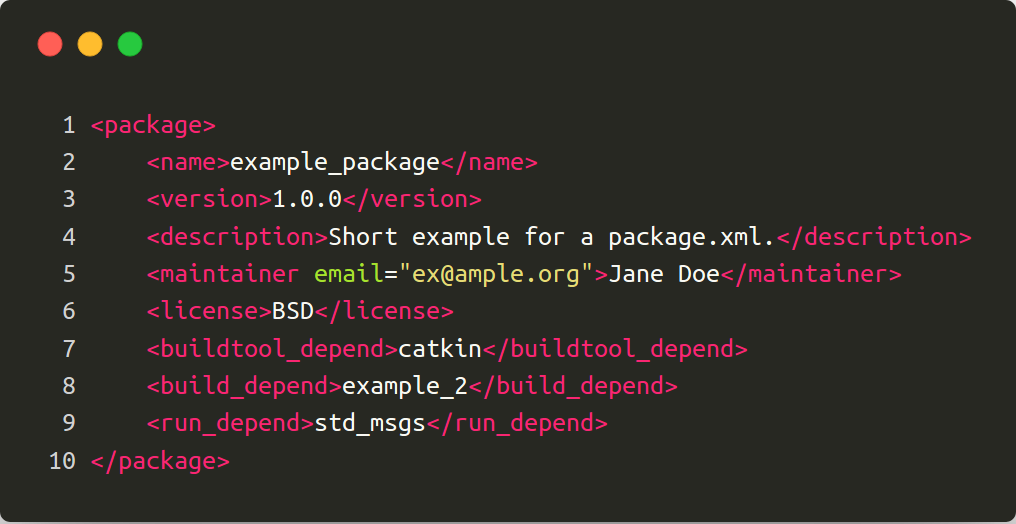
\includegraphics[width=0.8\textwidth]{chapter2/images/example_packagexml.png}
	\caption{ตัวอย่างไฟล์ package.xml แต่ละ tags สามารถใช้ในการบอกข้อมูลของ package นี้
	ใครเป็นเจ้าของ ใครเป็นคนเขียน รวมไปถึง dependencies ที่จำเป็นต้องใช้ของ package นี้ด้วย}
    \label{fig:example_packagexml}
\end{figure}

\subsubsection*{Code Distribution}
การที่จะนำ Nodes กลับมาใช้ใหม่หรือเอาออกมาแชร์ได้นั้น จะต้องมีการทำเอกสารของ Packages นั้นๆด้วย
โดยปกติแล้วจะถูกนำไปเก็บไว้ที่ GitHub และ package dependencies จะบอกไว้ในไฟล์ package.xml
เรียบร้อยแล้ว เพื่อให้ง่ายต่อการนำไปติดตั้ง หากผู้ที่นำไปใช้พัฒนาต่อหรือแก้ไขข้อผิดพลาดก็สามารถที่จะช่วยกันได้
โดยการ Pull request หรือ Report issues ได้

\subsubsection*{ROS Packages ที่ใช้ในงานวิจัย}
ในส่วนนี้จะอธิบายคร่าวๆถึง ROS standard packages ที่จะเอามาใช้ในงานวิจัยครั้งนี้
\paragraph*{rosbag}
rosbag เป็นแพกเกจที่สามารถบันทึก message ที่ส่งหากันในระหว่างที่ ROS กำลังทำงานได้
ไฟล์ที่บันทึกจะเรียกว่า rosbag ประโยชน์ของมันคือเราสามารถเอาเข้ามาใช้ในการตรวจสอบ
หรือนำมาเล่นซ้ำได้ อีกทั้งยังง่ายต่อการค้นหาข้อผิดพลาดอีกด้วย

\paragraph*{tf2}
tf2 เป็นแพกเกจที่สามารถติดตามการเปลี่ยนแปลงของ Coordinate frame เราสามารถใช้ในการหาความสัมพันธ์ระหว่าง
frame ได้ ยกตัวอย่างเช่นหากเราต้องการหาตำแหน่งของ foot เทียบกับ pelvis ก็สามารถใช้ tf2 หาได้

robot\_state\_publisher แพกเกจที่ subscribe JointState message เพื่อที่จะนำตำแหน่งของของข้อต่อ
และแปลงให้อยู่ในรูปข้อมูลของ tf2, tf2 สามารถเรียกจาก Node ใดๆก็ได้เพื่อที่จะหา Coordinate frame ที่ต้องการได้

\paragraph*{URDF}
Unified Robot Description Format (URDF) เป็นไฟล์ XML ที่เอาไว้อธิบายลักษณะของหุ่นยนต์
ใน ROS มีแพกเกจที่ใช้สำหรับการอ่านไฟล์ คือ urdf\_parser แต่ไฟล์นี้ก็มีการใช้งานโดย tf2 เช่นกัน

\paragraph*{xacro}
xacro เป็นไฟล์ XML เช่นเดียวกับ URDF โดยไฟล์ xacro นี้มีประโยชน์มากในการใช้งานใน ROS เพราะว่าทำให้การเขียนไฟล์
URDF ง่ายขึ้น เพราะสามารถทำเป็นมาโครได้ สามารถปรับแต่งค่าตัวแปรต่างๆได้ง่ายขึ้น

\subsubsection*{Visualization}
One of ROS’ core strengths is providing different tools for visualization.  Due to its
publisher-subscriber architecture, it is very easy to establish a data stream from the
program to the visualization.  Either the visualization can subscribe on topics that
are already being in use or additional topics can be provided from the software to
deliver more information to the visualization.  Messages in ROS are only published
if there is a subscriber on the topic, therefore publishing additional topics for visu-
alization reasons does not cost performance when the visualization is not running.
ROS provides two main tools for visualization which can be extended by plug-ins.
It is also possible to implement own tools which are independent from these.

\paragraph*{rqt}
rqt  is  a  QT  based  interface  with  ROS  connection \ref{fig:ros_gui_example}   Plug-ins  can  be
launched and provide a
QtWidget
.  Multiple widgets can be displayed at the same
time.  They can be resized and positioned by drag and drop.  ROS provides a set
of plug-ins but writing an own plug-in is possible too.  These plug-ins can be used
to visualize data in 2D but also to provide a controlling interface.  In the following,
some examples of important plug-ins are shown.
The
node
graph
plug-in shows all currently running nodes and topics.  Published
and subscribed topics are connected to their nodes and thereby it is easy to see the
flow of data.  This plug-in is especially helpful to get an overview of the running
software and to find misconnected nodes.
The
topic
monitor
lists all current topics.  It is possible to subscribe to them and
to get the current transmitted values.  Further on, statistics about the publishing
rate and the used bandwidth can be shown for each topic.
The
rqt
plot
plug-in  enables  live  plotting  of  data,  using
matplotlib
.    The
dynamic
reconfigure
plug-in provides an interface to change parameter values pre-
viously defined to be reconfigurable.  This is useful when tuning parameter values,
because  changing  it  is  possible  on  the  fly  and  does  not  require  a  restart  of  the
software


\begin{figure}[htbp]
    \centering
    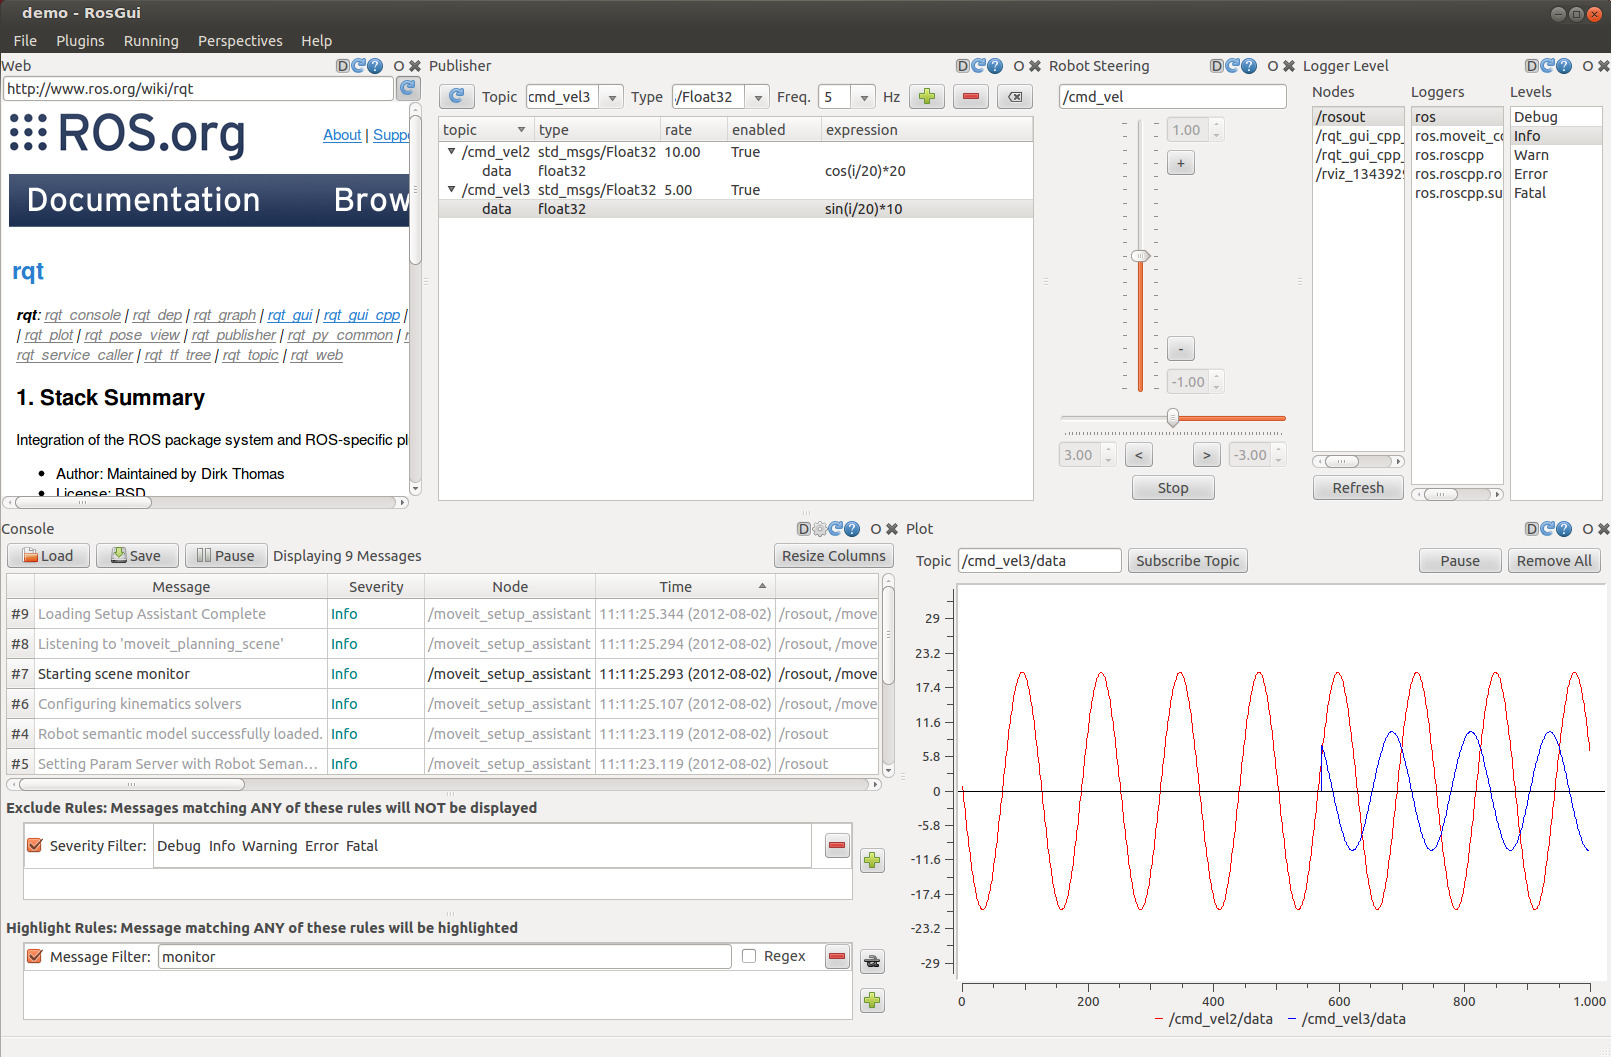
\includegraphics[width=0.8\textwidth]{chapter2/images/ros_gui_example.png}
	\caption{ตัวอย่างการแสดงผลใน rqt ในรูปเป็นการนำ rqt มาเขียนเป็น GUI ให้ผู้ใช้สามารถใช้งานได้ง่าย
	และสามารถที่จะปรับแต่ง parameters ต่างๆได้เรียลไทม์}
    \label{fig:ros_gui_example}
\end{figure}

\paragraph*{RViz}
RViz  provides  a  3D  visualization  of  the  robots  state  and  its  environment.   The
standardized URDF format is used to get a visual robot model, which is then used
to  show  the  current  positions  of  the  robots  joints.   Furthermore,  sensor  data  can
be displayed using marker messages.  These messages can be published by any node
and define three dimensional states which are displayed in RViz.  This is for example
helpful to get a visualization of recognized objects.  Furthermore, a lot of different
standard  ROS  messages  can  directly  be  visualized  in  RViz,  e.g.   camera  images,
depth  clouds,  laser  scans  and  point  clouds.   Thereby  RViz  provides  visualization
without additional effort, if the standard messages are used.  It is especially used for
localization and mapping, because it is possible to see the current sensor inputs of
the robot as well as its map in the same window \ref{fig:example_visualization_rviz}

\begin{figure}[htbp]
    \centering
    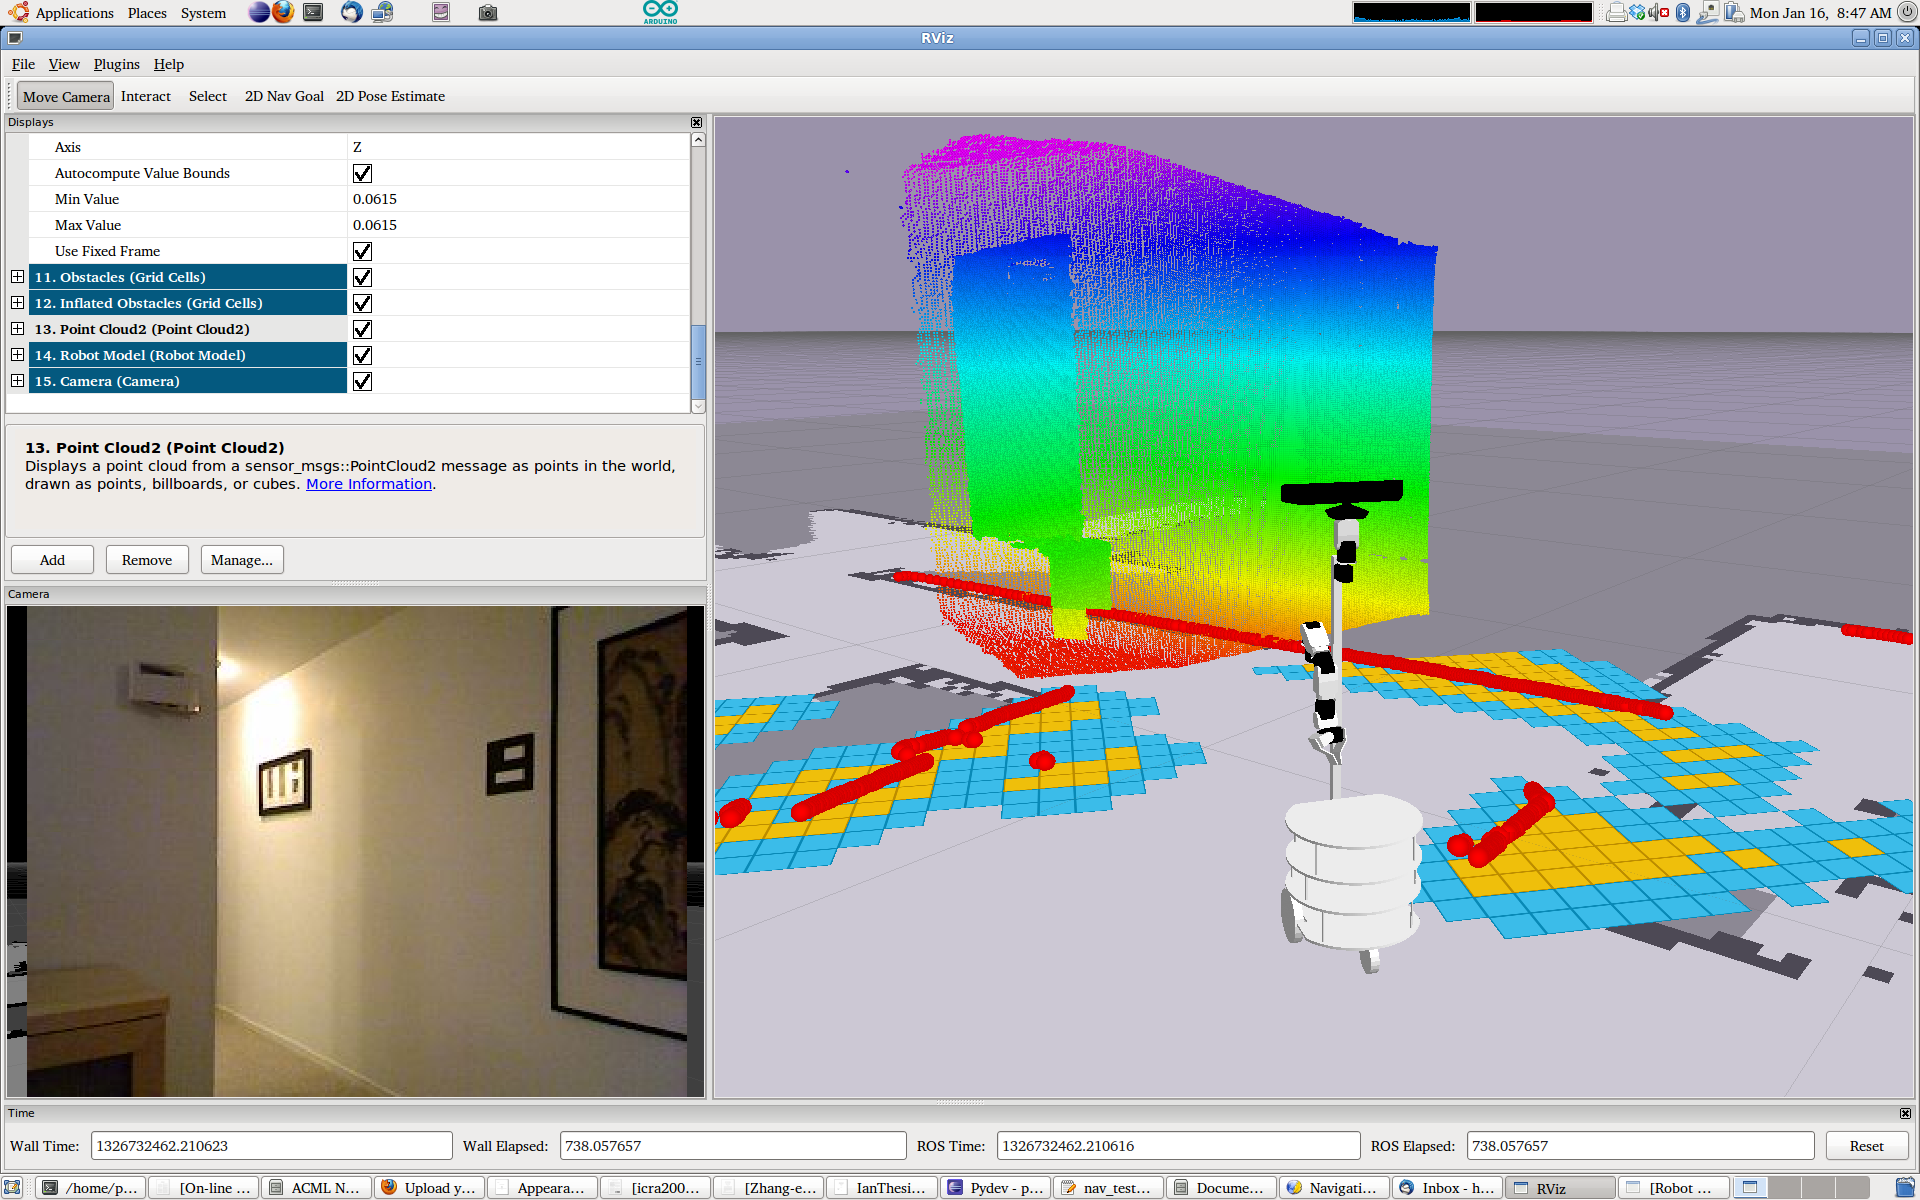
\includegraphics[width=0.8\textwidth]{chapter2/images/nav_test_rviz_2.png}
	\caption{ตัวอย่างการแสดงผลใน RViz ในรูปนี้เป็นเคสของหุ่นยนต์เคลื่อนที่ด้วยล้อ และทำแผนที่ด้วยข้อมูลความลึกที่ได้มาจาก Kinect}
    \label{fig:example_visualization_rviz}
\end{figure}



\subsubsection*{Simulation}
Simulation is a crucial part when developing robot software, since it gives the devel-
oper the possibility to run his software without using hardware.  This can prevent
hardware damages because bugs can be found before running it on the robot and
it can be used to accelerate development, e.g.  by testing in faster than real time.
While ROS can generally use any simulator, Gazebo is normally preferred, since it
has a good ROS integration and was also originally developed for ROS. In order to
use Gazebo, an URDF of the robot is required.
This  URDF  is  used  to  display  the  robot  in  the  simulator  and  to  compute  its
collisions with itself and the environment.  The simulator can provide sensor data
in  the  corresponding  standard  messages.   To  actuate  the  servos  of  the  robot,  dif-
ferent  controllers  are  available  which  work  with  the  corresponding  messages,  e.g.
JointTrajectory


\clearpage

\section{การออกแบบระบบพื้นฐาน}
\subsection{ข้อแตกต่างระหว่าง Open platform กับ Non-open platform}
\hspace*{10mm} หุ่นยนต์ Open platform คือ การออกแบบระบบพื้นฐานของหุ่นยนต์ที่เปิดให้ผู้ที่ต้องการศึกษาหรือผู้ใช้ทั่วไปสามารถเข้าถึงข้อมูลต่างๆที่เกี่ยวข้องกับหุ่นยนต์นั้นๆได้
ผู้ใช้สามารถที่จะนำข้อมูลเหล่านั้นมาแก้ไข ปรับปรุง แต่งเติม หรือเรียนรู้และพัฒนาตามได้ด้วยตนเอง 
ซึ่งข้อมูลที่กล่าวมานั้นสามารถหาได้จากเว็บไซต์ของผู้พัฒนาหุ่นยนต์ ปัจจุบันมีหุ่นยนต์ฮิวมานอยด์ที่เป็นเปิดให้เข้าถึงหลายรูปแบบแตกต่างกันไป \\
\hspace*{10mm} ส่วนหุ่นยนต์ Non-open source platform คือหุ่นยนต์ที่สร้างมาเฉพาะเจาะจงสำหรับการวิจัย การสำรวจ หรือการแข่งขันโดยเฉพาะ
ไม่เปิดให้บุคคลภายนอกเข้าศึกษาหรือแก้ไขปรับปรุง ซึ่งทำให้หุ่นยนต์ประเภทนี้ไม่เหมาะสำหรับผู้วิจัยที่จะเรียนรู้และศึกษาด้วยตนเอง เพราะมีขนาดใหญ่
ใช้ทรัพยากรมาก และการออกแบบมีความซับซ้อน เรียนรู้ยากกว่าหุ่นยนต์แบบ Open platform


% % ************************** Thesis Chapter3 **********************************
\chapter{การดำเนินงานวิจัย}

% \section{}
\section{หน้าที่ความรับผิดชอบ}
List are really easy to create
 
\begin{itemize}
  \item One entry in the list
  \item Another entry in the list
\end{itemize}

\section{การออกแบบโครงสร้างของหุ่นยนต์}
\subsection{การเชื่อมต่อหุ่นยนต์ฮิวมานอยด์}
โครงสร้างแพลตฟอร์มหุ่นยนต์อุทัยจะประกอบไปด้วยสองขา เพื่อทำให้เกิดองศาอิสระเป็น 12 องศาอิสระ
(DOFs) ใช้ Dynamixel servos 12 ตัว มอเตอร์ Dynamixel ทั้งหมดเชื่อมต่อกันแบบ daisy chain
ข้างนึงของมอเตอร์ตัวแรกเชื่อมต่อกับแบตเตอร์รี่ 12V และอีกข้างต่อกับ USB2Dynamixel
ทั้งหมดนี้เป็นการเชื่อมต่อ Odroid เข้ากับหุ่นยนต์ ดังรูปที่ \ref{fig:odroid2dynamixel}

\begin{figure}[htbp]
    \centering
    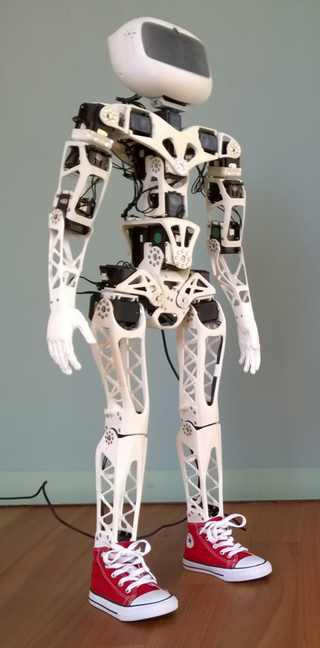
\includegraphics[width=0.3\textwidth]{chapter2/images/PoppyHumanoid1.png}
    \caption{การเชื่อมต่อระหว่าง Odroid กับ Dynamixel servos}
    \label{fig:odroid2dynamixel}
\end{figure}

หุ่นยนต์ฮิวมานอยด์อุทัยใช้เซอร์โวมอเตอร์ 12 ตัว ทำให้เกิดเป็น 12 องศาอิสระ
USB2Dynamixel ใช้เพื่อที่จะสั่งการเซอร์โวมอเตอร์ Dynamixel ผ่าน Odroid
ตำแหน่งของเซอร์โวมอเตอร์ Dynamixel EX-106+ นั้นมาจากเอนโคดเดอร์ที่อยู่ภายใน
เซนเซอร์ Gyro/Accelerometer ติดอยู่กับตัวของหุ่นยนต์ เพื่อช่วยในการทรงตัวของหุ่นยนต์
เซนเซอร์ Accelerometer จะอัพเดตค่าของตัวเองเรื่อยๆ ฟังก์ชั่นส่วนเสริมจะมาจาก ROS
และ Odroid เชื่อมต่อกับคอมพิวเตอร์ภายนอกผ่าน Wi-Fi

\subsection{อุปกรณ์ที่ใช้ในหุ่นยนต์ฮิวมานอยด์อุทัย}
\subsubsection*{Odroid}
\subsubsection*{Dynamixel servo EX-106+}
Dynamixel EX-106+ เป็นตัวขับเคลื่อนที่นิยมใช้ในปัจจุบัน โดยความสามารถของมันคือ สามารถที่จะอ่านค่าความเร็ว
แรงดันไฟฟ้า กระแสไฟฟ้า อุณหภูมิ ตำแหน่ง และแรงบิด มอเตอร์แต่ละตัวจะมีบอร์ดควบคุมของตัวเอง

\subsubsection*{USB2Dynamixel connector}
ตัวนี้เป็นอุปกรณ์สำหรับเชื่อมต่อ Odroid กับ Dynamixel โดยจะเชื่อมต่อผ่านพอร์ท USB ของ Odroid ไปยัง Dynamixel motor
ผ่านสายทั้งหมด 4 เส้น เป็นการเชื่อมต่อแบบ RS-485 
\subsubsection*{Accelerometer}
Accelerometer ที่ใช้เป็น MPU-9250 Accelerometer+Gyro+Magnito เพื่อเอาไว้ใช้หามุมเอียงของหุ่นยนต์
เทียบกับโลก
\subsubsection*{Ground contact sensor}
\subsubsection*{Wi-Fi Adapter}

\section{การออกแบบโปรแกรมด้วย ROS}
\subsection{Modelling}
หลังจากที่เราได้ออกแบบและโมเดลหุ่นยนต์ของเราขึ้นมาที่ใช้ CAD tools ต่างๆ เช่น AutoCAD, SolidWorks, Blender
หรืออื่นๆ ก็เพื่อที่จะนำมาใช้ในการทำ Simulation การที่เราทำ Simulation นั้นก็จะสามารถมองเห็นหุ่นยนต์
และเห็นการทำงานของหุ่นยนต์เราก่อนที่เราจะสร้างมันขึ้นมาจริงๆ หุ่นยนต์จำลองที่เราสร้างขึ้นมานั้นควรที่จะมีลักษณะให้ใกล้เคียงกับของจริงมากที่สุด
ไม่ว่าจะเป็นรูปร่าง รูปทรง น้ำหนักต่างๆ 

\subsubsection{ROS packages for robot modelling}
ROS นั้นได้ให้เครื่องมือที่ช่วยให้เราสามารถสร้าง 3D robot models ได้
ใน ROS มี meta package ที่ชื่อว่า robot\_model ซึ่งข้างในมี package ต่างๆที่ใช้สำหรับสร้าง 3D robot models
        
\paragraph*{urdf}
เป็น 1 ในหลายๆ package ที่อยู่ใน robot\_model, urdf เป็น xml ไฟล์ที่เอาไว้ใช้บอกลักษณะของหุ่นยนต์ ย่อมาจาก Unified Robot Description Format(URDF)
เราสามารถระบุ robot model, sensors และ working environment โดยใช้ URDF การบอกนั้นจะสามารถบอกเป็นเหมือน tree structure ของ link ต่างๆในตัวหุ่นยนต์ สามารถบอก rigid link เชื่อมต่อกันผ่าน joints แต่ถ้าเป็น flexible link จะไม่สามารถบอกได้โดยใช้ urdf

\subparagraph*{joint\_state\_publisher}
เครื่องมือนี้มีประโยชน์มากในการ model robot URDF เพราะมันสามารถหา joints ทุก joint ที่ไม่ใช่ fixed joints มาแสดงเป็น GUI sliders ทำให้เราสามารถเลื่อนๆหมุนๆไปมาได้ อีกทั้งยังสามารถใช้งานร่วมกับ visualize RViz

\subparagraph*{robot\_state\_publisher}
เป็นเครื่องมือที่ใช้ในการ publish 3d pose ของ link ต่างๆใน urdf การ ยublish นั้นจะใช้ ROS tf(transform) ROStf คือการหาความสัมพันธ์ระหว่าง frame ของหุ่นยนต์

\subparagraph*{xacro}
ย่อมาจาก XML Macros หรือเราสามารถเรียกอีกอย่างว่า URDF plus add-ons. ซึ่งการทำงานเหมือนกับ urdf แต่ทำให้ไฟล์ urdf สั้นกว่า อ่านง่ายกว่า และสามารถใช้เพื่อทำให้สร้างหุ่นยนต์ที่มีความซับซ้อนง่ายขึ้น เราสามารถแปลงไฟล์ xacro เป็น urdf ได้

\subsubsection{URDF}
ในส่วนนี้จะเป็นการอธิบายระบบทางกลของหุ่นยนต์ฮิวมานอยด์เป็นไฟล์ที่ใช้ร่วมกับ ROS ได้ เพื่อที่จะสามารถนำไปใช้กับ Simulation ในอนาคตได้
ในการอธิบายระบบทางกลนั้นผู้วิจัยได้ใช้ไฟล์ URDF (Universal Robotics Description Format) ซึ่งใช้ภาษาการเขียนเป็น XML ในการบอกส่วนประกอบแต่ละส่วนของหุ่นยนต์

\subsubsection*{Link}
ในไฟล์ URDF แต่ละชิ้นส่วนของหุ่นยนต์เราจะเรียกว่า link แล้วใน link จะประกอบไปด้วยส่วนย่อยๆ
3 ส่วนคือ <inertia> ที่เอาไว้บอกถึงค่าตัวแปรทางฟิสิกส์, <visual> ที่เอาไว้แสดงผลให้เราเห็น, 
<collision> ที่เอาไว้ตรวจสอบว่าหุ่นยนต์มีการชนกันกับสิ่งแวดล้อมไหม ดังตัวอย่างด้านล่างนี้

% \begin{verbatim}
% <link name="my_link">
%     <inertia>
%         <origin xyz="0 0 0.5" rpy="0 0 0"/>
%         <mass value="1"/>
%         <inertia ixx="100" ixy="0" ixz="0" iyy="100" iyz="0" izz="100"/>
%     </inertia>
%     <visual>
%         <origin xyz="0 0 0" rpy="0 0 0"/>
%         <geometry>
%             <box size="1 1 1" />
%         </geometry>
%         <material name="Cyan">
%             <color rgba="0 1.0 1.0 1.0"/>
%         </material>
%     </visual>
%     <collision>
%         <origin xyz="0 0 0" rpy="0 0 0"/>
%         <geometry>
%             <cylinder radius="1" length="0.5"/>
%         </geometry>
%     </collision>
% </link>
% \end{verbatim}

ยังมี tags อีกหลายตัวที่ใช่ในการอธิบายแต่ละชิ้นส่วนของหุ่นยนต์ แต่ตัวอย่างเป็นเพียงแค่ส่วนหนึ่งเท่านั้น
ในความเป็นจริงแล้วเราจะเขียน tags ต่างๆก็ตามที่เราต้องการ โดยใน URDF ไฟล์นั้นจะเอาไว้เก็บข้อมูลลักษณะเฉพาะของหุ่นยนต์เอาไว้
และยังสามารถใช้กับซอฟแวร์ตัวอื่นๆอีกได้
\begin{figure}[h]
	\centering
	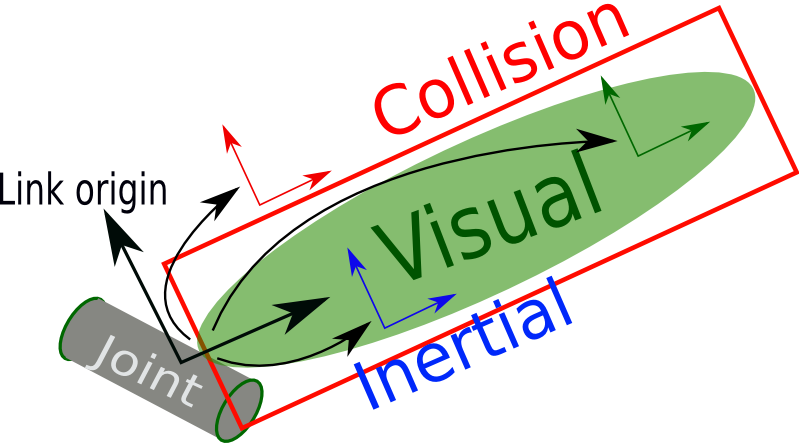
\includegraphics[width=0.45\textwidth]{chapter3/images/urdf_link.png}
	\caption{การอธิบาย link ใน URDF ไฟล์}
	\label{fig:urdf_link}
\end{figure}

\subsubsection*{Joint}
อีกส่วนที่สำคัญสำหรับการสร้างไฟล์หุ่นยนต์ด้วย URDF ก็คือ Joint tag โดย tag นี้จะอธิบายถึงความสัมพันธ์ระหว่างก้านต่อสองอัน
ส่วนนี้ไม่ได้มีเพียงแค่ทำข้อต่อให้เป็นแบบหมุนได้อย่างเดียว ยังมี Fix, Revolution, Linear และ Planar นอกเหนือจากนี้
เรายังสามารถที่จะเพิ่มองศาสูงสุดต่ำสุดของข้อต่อ รวมไปถึง dynamic properties ต่างๆ ตามที่เห็นตัวอย่างด้านล่างนี้

% \begin{verbatim}
% <joint name="my_joint" type="floating">
% <origin xyz="0 0 1" rpy="0 0 3.1416"/>
% <parent link="link1"/>
% <child link="link2"/>
% <calibration rising="0.0"/>
% <dynamics damping="0.0" friction="0.0"/>
% <limit effort="30" velocity="1.0" lower="-2.2" upper="0.7"/>
% <safety_controller k_velocity="10" k_position="15" soft_lower_limit="-2.0" soft_upper_limit="0.5"/>
% </joint>
% \end{verbatim}

เมื่อเรานำ Joint และ Link มารวมกันเราจะต้องพิจารณาว่ามีวางรูปแบบเป็นไปตามรูปที่ \ref{fig:urdf_joint}
โดยจะมีระยะระหว่างแกนของแต่ละข้อต่อกับก้านต่อ ชิ้นส่วนแรกของการสร้างไฟล์ URDF จะมีชื่อว่า base\_link
และเฟรม origin จะเป็นเฟรมอ้างอิง เมื่อเราต่อ Joint เข้ากับ Link จะเรียกก้านต่อที่เอามาติดว่า parent
โดยเฟรม origin ของข้อต่อจะอยู่จุดเดียวกับเฟรม origin ของก้านต่อ ในสถานะเดียวกันก้านต่อที่นำมาต่อจากข้อต่อ
เราจะเรียกว่า child และเฟรม origin ของก้านต่อ child จะอยู่ที่จุดเดียวกับเฟรม origin ของข้อต่อ

\begin{figure}[h]
	\centering
	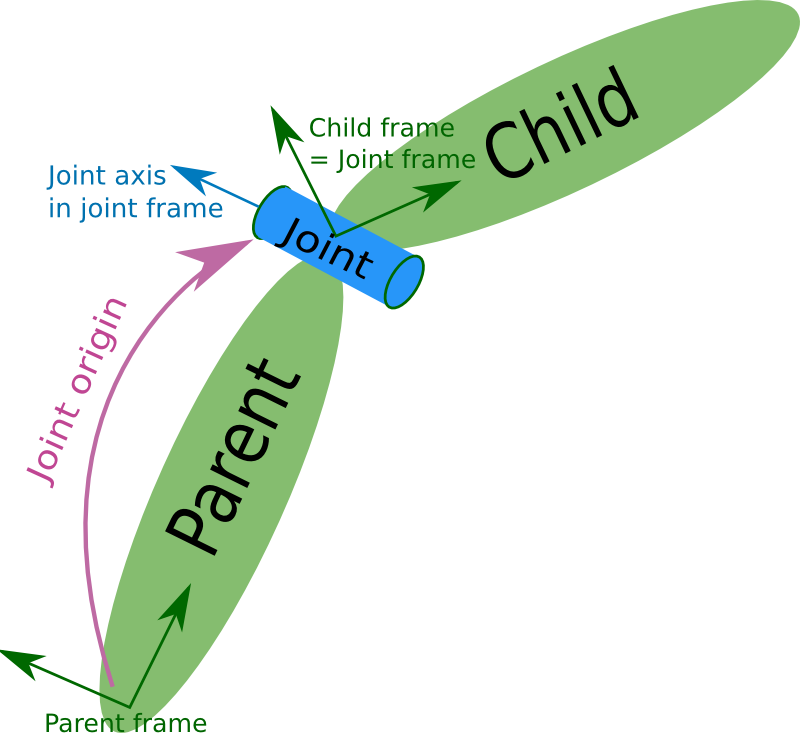
\includegraphics[width=0.45\textwidth]{chapter3/images/urdf_joint.png}
	\caption{การอธิบาย Joint ใน URDF ไฟล์}
	\label{fig:urdf_joint}
\end{figure}

\section{การออกแบบระบบพื้นฐาน}
\subsection*{UTHAI-Tools}
เครื่องมือสำหรับการทำงานในฮิวมานอยด์

\subsubsection*{sketch-lib}
เป็นเครื่องมือที่ใช้สำหรับเอาไว้วาดรูปเฟรมของหุ่นยนต์

\begin{figure}[htbp]
	\centering
	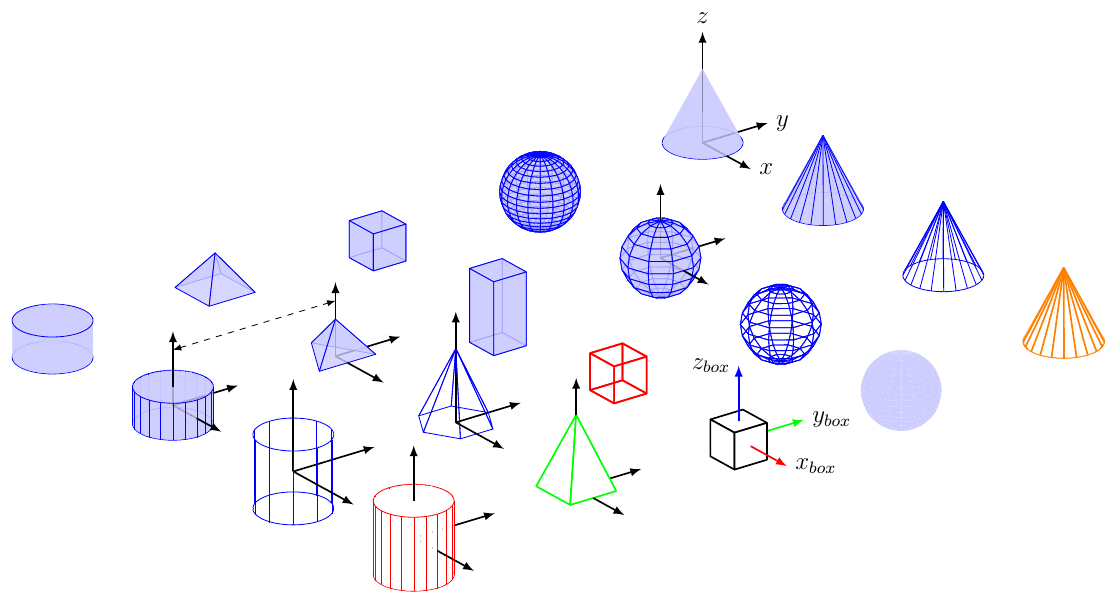
\includegraphics[width=0.7\textwidth]{chapter3/images/basic-shapes.png}
	\caption{ภาพตัวอย่างการวาดออฟเจ็คต่างๆ}
	\label{fig:basic-shapes_sk}
\end{figure}
\begin{figure}[htbp]
	\centering
	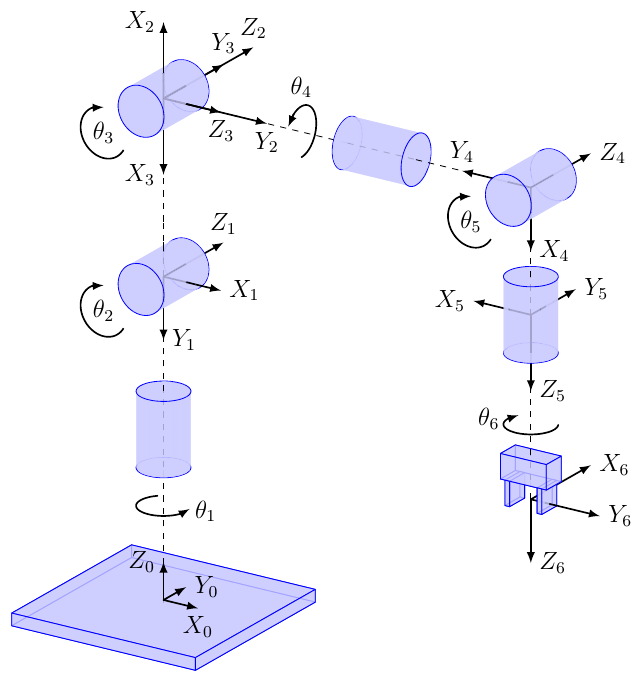
\includegraphics[width=0.5\textwidth]{chapter3/images/test_robot.png}
	\caption{ภาพตัวอย่างการวาดเฟรมของแขนกล}
	\label{fig:test-robot_sk}
\end{figure}
\begin{figure}[htbp]
	\centering
	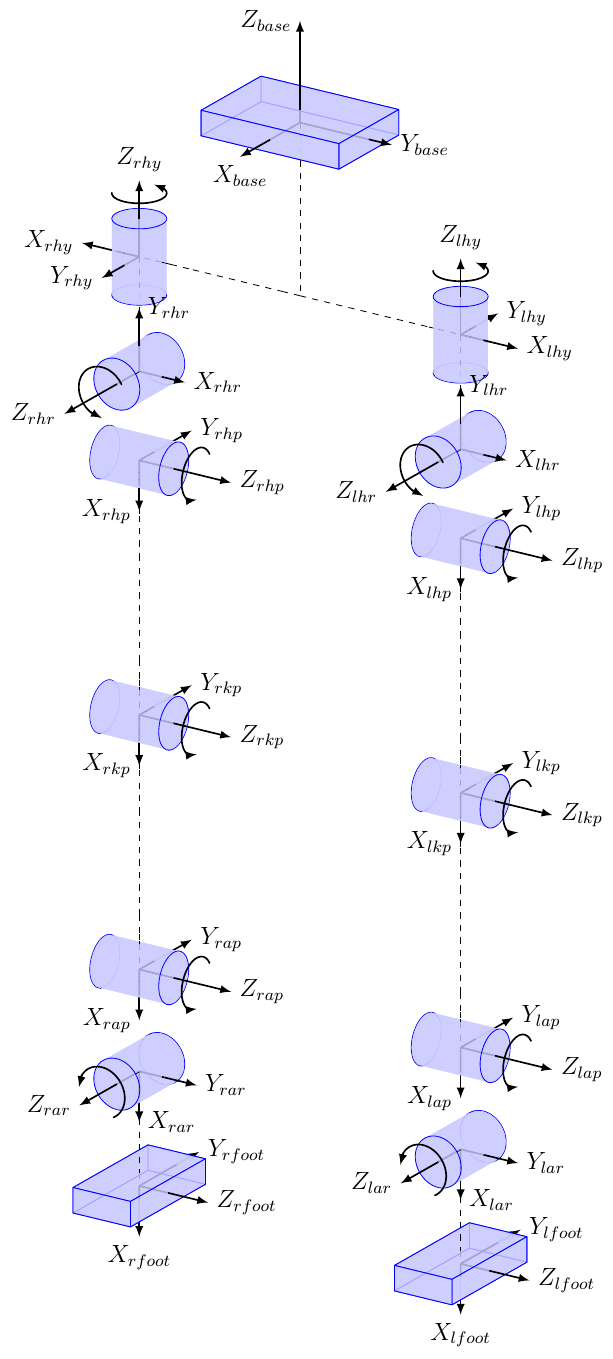
\includegraphics[width=0.4\textwidth]{chapter3/images/uthai_kinematics.png}
	\caption{ภาพตัวอย่างการวาดเฟรมของหุ่นยนต์ฮิวมานอยด์}
	\label{fig:uthai_kinematics_sk}
\end{figure}

% % ************************** Thesis Chapter4 **********************************
\chapter{ผลการดำเนินงาน}
\section{โครงสร้างของหุ่นยนต์}
\begin{figure}[!ht]
  \centering
  \begin{subfigure}[b]{0.2\linewidth}
    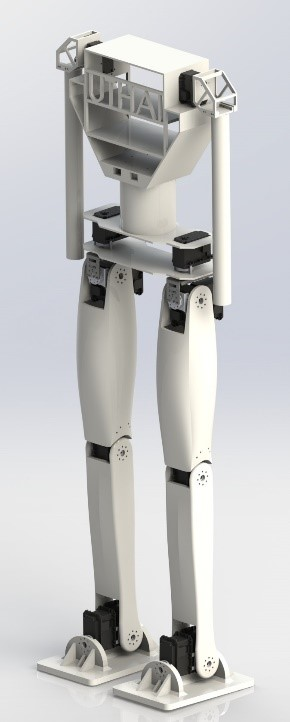
\includegraphics[width=\linewidth]{chapter4/images/UTHAI_ver_1.jpg}
    \caption{โครงสร้างหุ่นยนต์ในโปรแกรม 3 มิติ(ครั้งที่ 1)}
  \end{subfigure}
  \begin{subfigure}[b]{0.175\linewidth}
    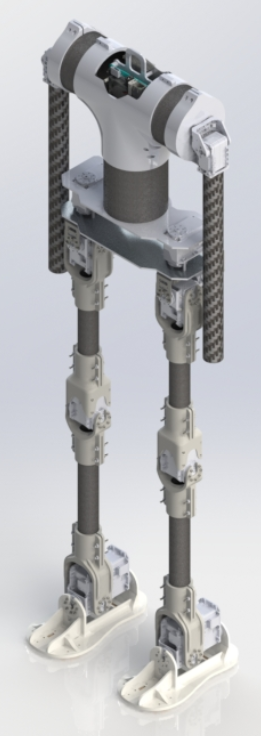
\includegraphics[width=\linewidth]{chapter4/images/uthai_humanoid.PNG}
    \caption{โครงสร้างหุ่นยนต์ในโปรแกรม 3 มิติ(ครั้งที่ 2)}
  \end{subfigure}
  \caption{รูปการออกแบบโครงสร้างหุ่นยนต์ในโปรแกรม 3 มิติ}
  \label{fig:UTHAI_humanoid}
\end{figure}

โครงสร้างของหุ่นยนต์ฮิวมานอยด์ UTHAI จะแบ่งออกเป็น 2 ส่วนคือ ส่วนท่อนบนและส่วนท่อนล่างโดยส่วนท่อนบนจะประกอบไปด้วย 
เอว ลำตัว แขน และท่อนล่างจะประกอบไปด้วย สะโพก ขา น่อง ฝ่าเท้า
ในการเลือกใช้วัสดุนั้นได้แสดง ดังตารางที่ \ref{tab:UTHAI_material_x}

\begin{table}[ht]
	\centering
	\begin{tabular}{| l | l |}
		\hline
		ชิ้นส่วน & วัสดุที่ใช้ขึ้นรูป \\
        \hline
        แขน	& ท่อคาร์บอนไฟเบอร์ ขนาด 30 มม. \\
        ลำตัว & เครื่องพิมพ์ 3 มิติ โดยใช้วัสดุ PLA \\
        เอว	& ท่อคาร์บอนไฟเบอร์ ขนาด 88 มม. \\
        สะโพก & อลูมิเนียมอัลลอยพับ \\
        น่อง & เครื่องพิมพ์ 3 มิติ โดยใช้วัสดุ PLA \\
        ขา & เครื่องพิมพ์ 3 มิติ โดยใช้วัสดุ PLA \\
        ฝ่าเท้า	& เครื่องพิมพ์ 3 มิติ โดยใช้วัสดุ PLA \\
	    \hline
	\end{tabular}
	\caption{ตารางแสดงวัสดุที่ใช้ขึ้นรูปหุ่นยนต์ฮิวมานอยด์ UTHAI}
	\label{tab:UTHAI_material_x}
\end{table}

ซึ่งในการออกแบบนี้ได้แบ่งการออกแบบออกเป็น 2 ครั้งด้วยกันเนื่องจากว่าเกิดปัญหาในด้านน้ำหนักของการออกแบบครั้งที่ 1 ที่มากเกินไป
จึงทำการปรับปรุงใหม่เพื่อให้มีน้ำหนักที่เบามากขึ้นกว่าเดิม แต่ยังคำนึงถึงความแข็งแรงของโครงสร้างให้ไม่น้อยไปกว่าเดิม 
\clearpage
\subsection{การออกแบบขา}
\subsubsection{การออกแบบโครงสร้างส่วนขาครั้งที่ 1}
การออกแบบโครงสร้างส่วนขาของหุ่นยนต์ฮิวมานอยด์ ได้ออกแบบโดยคำนึงถึงการขึ้นรูปด้วยเครื่องพิมพ์สามมิติ 
แต่เนื่องจากว่าเครื่องพิมพ์สามมิติที่ใช้ในการผลิตนั้นมีขนาดที่เล็กกว่าขนาดที่จะพิมพ์จริงจึงต้องทำการแยกส่วนของขาออก
เป็นจำนวน 2 ส่วนในแต่ละในก้านต่อของขาท่อนบนและขาท่อนล่าง และหลังจากนั้นใช้การยึดชิ้นส่วนด้วยการตอกสลักเพื่อยึดติดชิ้นส่วนเข้าด้วยกัน
เพื่อให้มีความแข็งแรงมากกว่าการต่อแบบทั่วไป ดังรูปที่ \ref{fig:leg_x} เมื่อทำการพิมพ์ชิ้นงานส่วนขาท่อนบนและท่อนล่าง
ออกมาจะได้น้ำหนักของชิ้นงานตามตาราง \ref{tab:UTHAI_leg}


\begin{figure}[!ht]
    \centering
    \begin{subfigure}[b]{0.3\linewidth}
      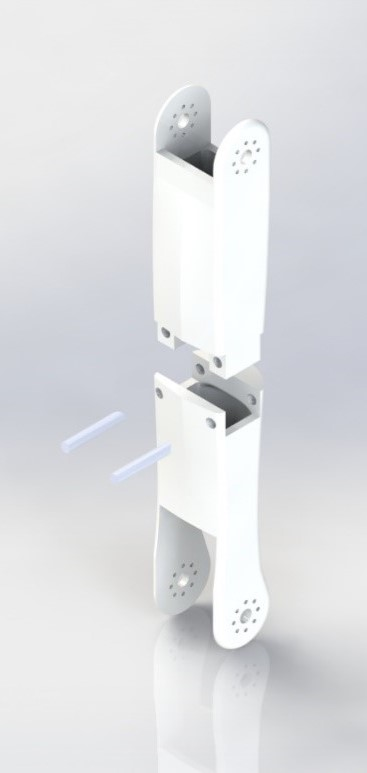
\includegraphics[width=\linewidth]{chapter4/images/shin.jpg}
      \caption{โครงสร้างส่วนหน้าแข้ง}
    \end{subfigure}
    \begin{subfigure}[b]{0.35\linewidth}
      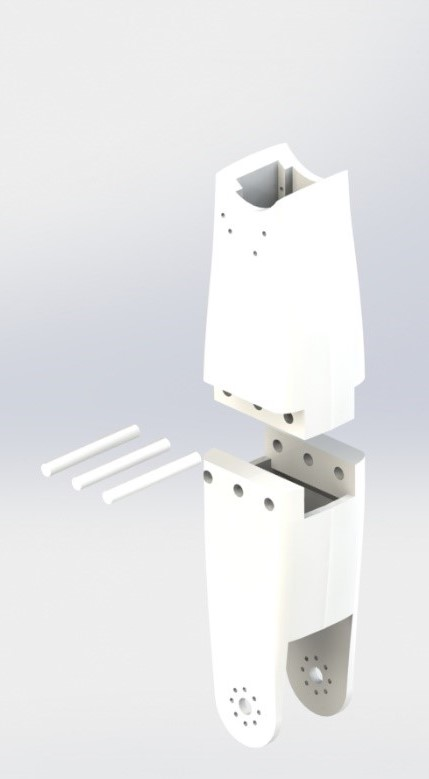
\includegraphics[width=\linewidth]{chapter4/images/thigh.jpg}
      \caption{โครงสร้างส่วนต้นขา}
    \end{subfigure}
    \caption{รูปการออกแบบส่วนขาของหุ่นยนต์ฮิวมานอยด์ UTHAI}
    \label{fig:leg_x}
  \end{figure}

\begin{table}[ht]
	\centering
	\begin{tabular}{| l | l |}
		\hline
		ชิ้นส่วน & น้ำหนัก (กรัม) \\
        \hline
        ต้นขา & 263 \\
        หน้าแข้ง & 204 \\
	    \hline
	\end{tabular}
	\caption{ตารางแสดงน้ำหนักของชิ้นส่วนขา}
	\label{tab:UTHAI_leg}
\end{table}

จากการทดสอบความสามารถในการเคลื่อนที่ พบว่าตัวขับเคลื่อนสามารถเคลื่อนที่เข้าตำแหน่งได้ถูกต้องตามมุม 
ที่ป้อนเข้าไปให้ระบบ แต่หากทำให้ชิ้นส่วนของขาเคลื่อนที่ด้วยถี่ไปกลับสูงและด้วยความเร็วที่มาก จะทำให้ตัวขับเคลื่อนเกิดการโอเวอร์โหลด 
ซึ่งมีผลทำตัวขับเคลื่อนหยุดการทำงาน ซึ่งต้องทำการปิดเปิดตัวขับเคลื่อนใหม่

\clearpage
\subsubsection*{ผลการทดสอบ}
จากการทดสอบความแข็งแรงของชิ้นงาน พบว่าชิ้นงานมีความแข็งแรงเพียงพอที่จะทำให้ตัวขับเคลื่อนมีค่าแรงบิดเป็นค่าแรงบิดสูงสุด(Stall Torque)
แล้วทำให้ชิ้นงานไม่เกิดความเสียหาย

จากการทดสอบระยะเวลาการทำงานของตัวขับเคลื่อน ด้วยการเขียนโปรแกรมให้ตัวขับเคลื่อน เคลื่อนที่ไปกลับ สลับตำแหน่งไปเรื่อยๆอย่างต่อเนื่อง เป็นเวลา 20 นาที
พบว่า ตัวขับเคลื่อนทำงานได้เป็นปกติ

\subsubsection*{ปัญหาที่พบในการออกแบบครั้งที่ 1}
เนื่องจากว่าเป้าหมายของการสร้างหุ่นยนต์ตัวนี้ให้มีน้ำหนักที่เบา (น้อยกว่า 5 กิโลกรัม) จึงพบปัญหาว่า
น้ำหนักของส่วนขาที่ได้ออกแบบมานั้นมีน้ำหนักมากเกินกว่าของหุ่นยนต์กนก (ชื่อหุ่นยนต์ตัวเดิมก่อนจะเป็นอุทัย)
ซึ่งเป็นผลทำให้เกิดปํญหาเรื่องภาระโหลดของดิจิตอลเซอร์โว ที่ต้องกระทำที่มีมากขึ้นจากเดิมและจะทำให้น้ำหนักของตัวหุ่นยนต์มากขึ้น 
เมื่อเปรียบเทียบผลลัพธ์น้ำหนักส่วนขาของหุ่นยนต์กนกกับหุ่นยนต์ฮิวมานอยด์ UTHAI ได้ผลดังตารางที่ \ref{tab:UTHAI_KANOK_Comp}

\begin{table}[ht]
	\centering
	\begin{tabular}{| l | l | l |}
		\hline
        ชิ้นส่วน & หุ่นยนต์กนก (เดิม)(กรัม) & หุ่นยนต์ UTHAI \\
        \hline
        ขาท่อนบน & 171 & 263 \\
        ขาท่อนล่าง & 172 & 204 \\
	    \hline
	\end{tabular}
	\caption{ตารางเปรียบเทียบน้ำหนักของชิ้นส่วนขาของหุ่นยนต์}
	\label{tab:UTHAI_KANOK_Comp}
\end{table}

จากข้อมูลในตารางนั้นจะเห็นได้ว่า หนักที่เพิ่มขึ้นมากจากการออกแบบใหม่แต่ละชิ้นนั้น มากถึง 124 กรัม
ต่อขา 1 ข้าง และ 248 กรัมเมื่อเทียบกับขาทั้งหมดและเปรียบเทียบกับข้อมูลก่อนหน้า

หลังจากพบปัญหาดังกล่าวผู้จัดทำจึงได้ตัดสินใจทำการเปลี่ยนวัสดุที่ใช้ทำโครงสร้างในครั้งแรก
ที่จะใช้การขึ้นรูปชิ้นงานด้วยการพิมพ์ขึ้นรูป 3 มิติ มาเป็นวัสดุผลระหว่างคาร์บอนไฟเบอร์และชิ้นงาน 3 มิติแทน
โดยจะให้ชิ้นงาน 3 มิตินั้นทำหน้าที่เป็นตัวเชื่อมระหว่างวัสดุคาร์บอนไฟเบอร์กับมอเตอร์ และยึดกับวัสดุคาร์บอนไฟเบอร์ด้วยการบีบ
ซึ่งเหตุผลที่ต้องทำเช่นนี้เพราะต้องการลดน้ำหนักของหุ่นยนต์ลง เพื่อไม่ให้มอเตอร์รับภาระที่หนักเกินไป 

\begin{table}[ht]
	\centering
	\begin{tabular}{| l | l | l |}
		\hline
		ชิ้นส่วน & วัสดุที่ใช้ขึ้นรูป (เก่า) & วัสดุที่ใช้ขึ้นรูป (ใหม่) \\
        \hline
        แขน	& ท่อคาร์บอนไฟเบอร์ ขนาด 30 มม. & เดิม\\
        ลำตัว & เครื่องพิมพ์ 3 มิติ โดยใช้วัสดุ PLA & เดิม\\
        เอว	& ท่อคาร์บอนไฟเบอร์ ขนาด 88 มม. & เดิม\\
        สะโพก & อลูมิเนียมอัลลอยพับ & เดิม\\
        น่อง & เครื่องพิมพ์ 3 มิติ โดยใช้วัสดุ PLA & วัสดุผสมระหว่างคาร์บอนไฟเบอร์และ ชิ้นงาน 3 มิติ \\
        ขา & เครื่องพิมพ์ 3 มิติ โดยใช้วัสดุ PLA  & วัสดุผสมระหว่างคาร์บอนไฟเบอร์และ ชิ้นงาน 3 มิติ\\
        ฝ่าเท้า	& เครื่องพิมพ์ 3 มิติ โดยใช้วัสดุ PLA & เดิม\\
	    \hline
	\end{tabular}
	\caption{ตารางแสดงวัสดุที่แก้ไขในการใช้ขึ้นรูป UTHAI }
	\label{tab:UTHAI_materialchange}
\end{table}

\clearpage
\subsubsection{การออกแบบโครงสร้างส่วนขาครั้งที่ 2}
ครั้งนี้การออกแบบชิ้นส่วนขาของหุ่นยนต์นั้น ได้คำนึงถึงเรื่องน้ำหนักเป็นหลัก และยังคงให้ความสำคัญกับข้อต่อที่จะใช้รับน้ำหนักทั้งตัวหุ่นยนต์
และยังคงรับแรงบิดของมอเตอร์อีกด้วย ดังนั้นจึงได้ตัดสินใจที่จะเปลี่ยนจากการใช้วัสดุจากการพิมพ์สามมิติ  ซึ่งเป็นพลาสติกทั้งหมด มาเป็นวัสดุผสม 
ระหว่างคาร์บอนไฟเบอร์กับชิ้นส่วนการพิมพ์สามมิติ ซึ่งขึ้นรูปจากพลาสติก PLA และทำการยึดติดกันด้วยการบีบอัด ดังรูปที่ \ref{fig:newleg}
เมื่อทำการพิมพ์ชิ้นงานส่วนขาท่อนบนและท่อนล่างและทำการประกอบ จะได้น้ำหนักของชิ้นงานเปรียบเทียบกับของเดิม ดังตารางที่ \ref{tab:UTHAI_leg_compilation}

\begin{figure}[!ht]
    \centering
    \begin{subfigure}[b]{0.3\linewidth}
      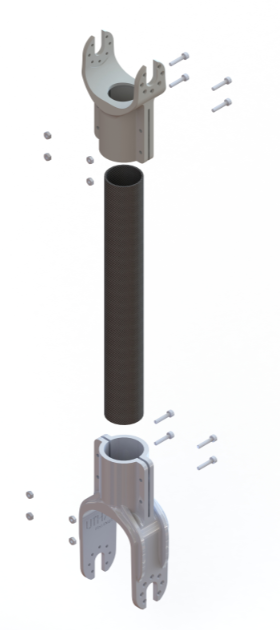
\includegraphics[width=\linewidth]{chapter4/images/carb_shin.PNG}
      \caption{โครงสร้างส่วนหน้าแข้ง (ใหม่)}
    \end{subfigure}
    \begin{subfigure}[b]{0.3\linewidth}
      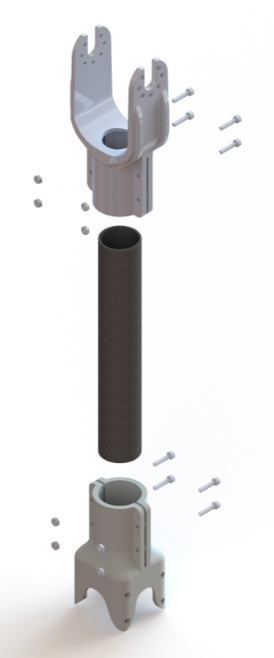
\includegraphics[width=\linewidth]{chapter4/images/carb_thigh.PNG}
      \caption{โครงสร้างส่วนต้นขา (ใหม่)}
    \end{subfigure}
    \caption{รูปการออกแบบส่วนขาของหุ่นยนต์ฮิวมานอยด์ UTHAI (ใหม่)}
    \label{fig:newleg}
  \end{figure}

\begin{table}[!ht]
	\centering
	\begin{tabular}{| l | l | l |}
		\hline
		ชิ้นส่วน & น้ำหนักเดิม (กรัม) & น้ำหนักใหม่ (กรัม) \\
        \hline
        ต้นขา & 263 & 161\\
        หน้าแข้ง & 204 & 166\\
	    \hline
	\end{tabular}
	\caption{ตารางแสดงน้ำหนักเปรียบเทียบของชิ้นส่วนขา}
	\label{tab:UTHAI_leg_compilation}
\end{table}  

\clearpage
\subsubsection*{การขึ้นรูปชิ้นงาน}
การขึ้นรูปชิ้นงานนนั้น ได้ใช้การขึ้นรูปชิ้นตามความสูงแนวแกน Z ดังรูปที่ \ref{fig:print_axis} เพื่อให้ชิ้นงานมีความสวยงามและสามารถสวมได้พอดี
กับท่อนคาร์บอนโดยให้มีผิวสัมผัสมากที่สุด ในการยึดเกาะ\footnote{Experimental Characterization of the Mechanical Properties of 3D-Printed ABS and Polycarbonate Parts}
\begin{figure}[!ht]
    \centering
    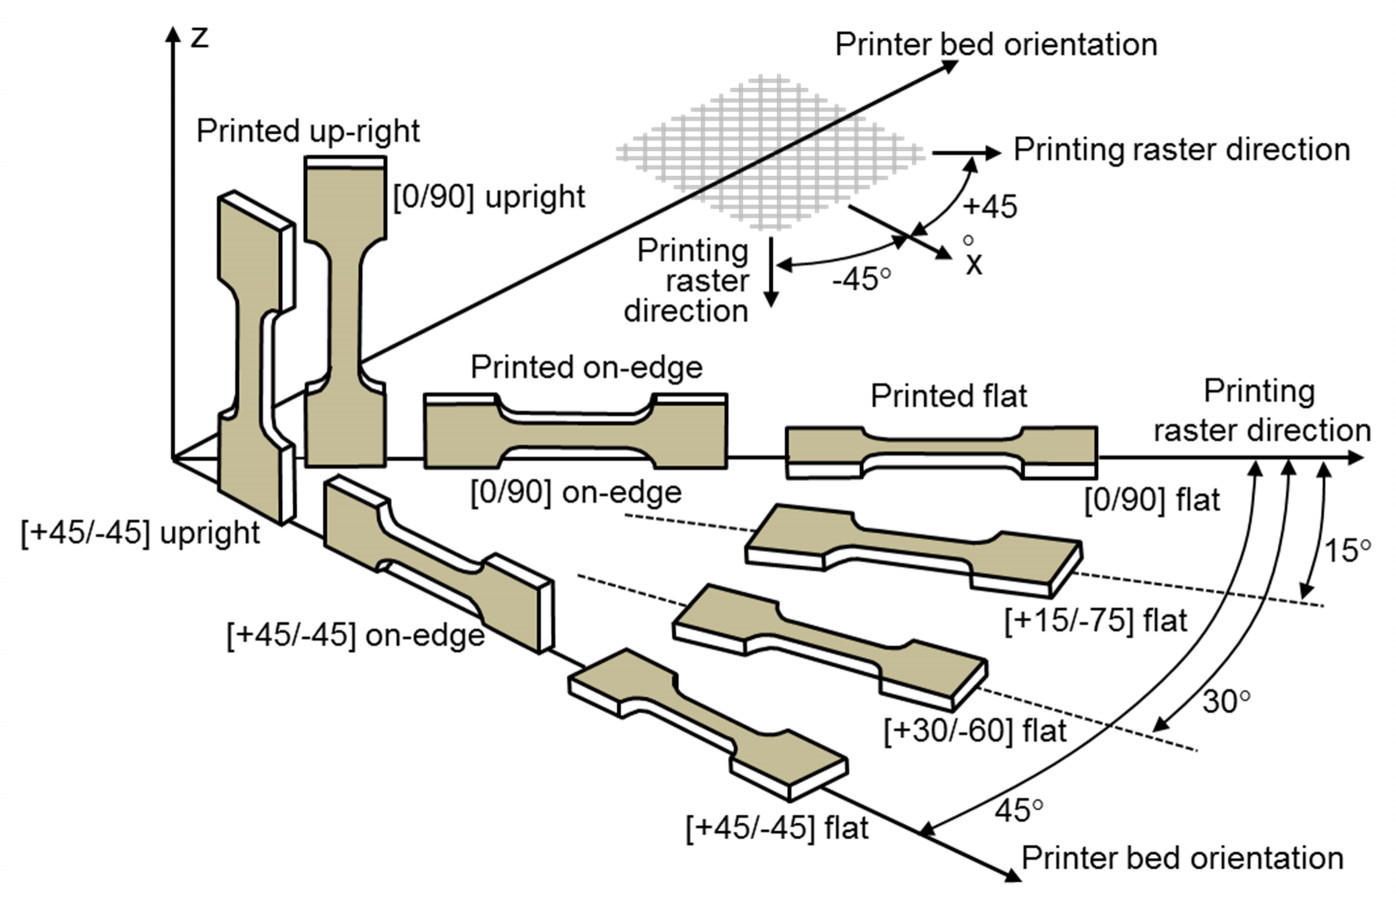
\includegraphics[width=0.6\textwidth]{chapter4/images/print_axis.png}
    \caption{รูปการชิ้นรูปชิ้นงานด้วยการพิมพ์งานสามมิติ }
    \label{fig:print_axis}
\end{figure}

\subsubsection{ทดสอบโครงสร้างและการขับเคลื่อน}	
จากการทดสอบความแข็งแรงของวัสดุโดยการนำไปประกอบกับตัวหุ่นยนต์จริง และทำการทดลองเดินพบว่าเมื่อทำการเดินจริงนั้น 
เกิดการฉีกขาดของชิ้นงานที่ ชั้นการพิมพ์ของชิ้นงาน ดังรูปที่ \ref{fig:fatiguelayer_1} ซึ่งเกิดจากการได้รับแรงบิดมากเกินไปจากน้ำหนักของชิ้นงานส่วนขา
และแรงที่ชิ้นงานจะได้รับนั้น จะเป็นเพียงส่วนการเชื่อมกันติดของชั้นพลาสติกเท่านั้น ที่นี้เส้นพลาสติกจะไม่ได้เป็นตัวรับแรงจึงทำให้
เกิดการเปราะหักที่ง่ายกว่าดังนั้นจึงทำการออกแบบใหม่โดยการเพิ่มสันให้ชิ้นงานและเพื่มความหนาบนหน้าแปลนเชื่อมกับตัวมอเตอร์
และทำการขึ้นรูปชิ้นงาน โดยให้ความสูงของชิ้นงานเป็นไปตามแกน X และทำการเติมเนื้อพลาสติกด้านในให้เต็ม 100\% ดังรูปที่ \ref{fig:fatiguelayer}
\begin{figure}[!ht]
    \centering
    \begin{subfigure}[b]{0.225\linewidth}
      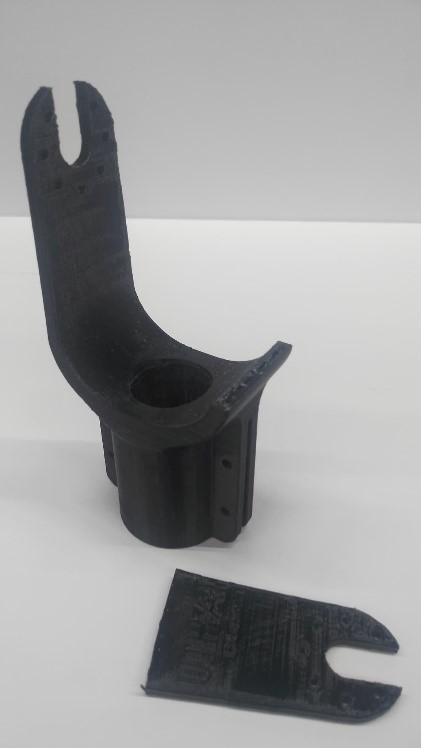
\includegraphics[width=\linewidth]{chapter4/images/fatigue1.jpg}
      \caption{รูปแสดงการแตกหักของชิ้นงาน}
      \label{fig:fatiguelayer_1}
    \end{subfigure}
    \begin{subfigure}[b]{0.3\linewidth}
      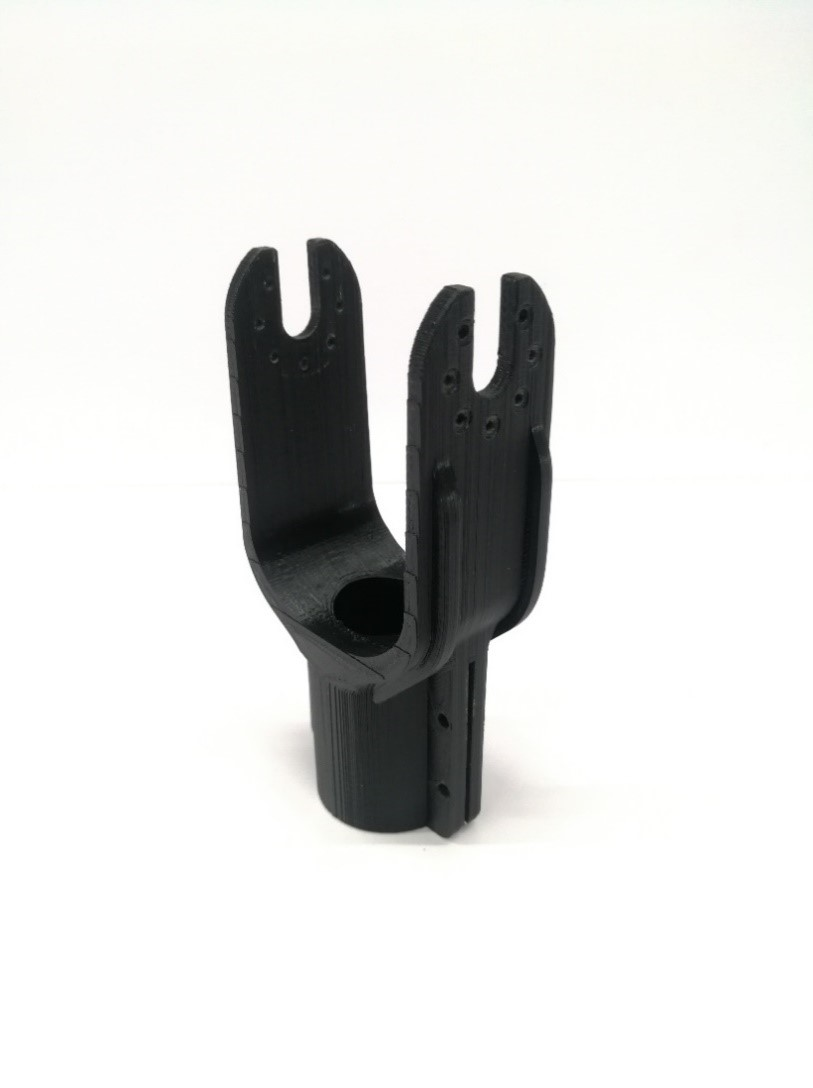
\includegraphics[width=\linewidth]{chapter4/images/fatigue2.jpg}
      \caption{รูปแสดงชิ้นงานที่ทำการออกแบบใหม่}
    \end{subfigure}
    \begin{subfigure}[b]{0.38\linewidth}
        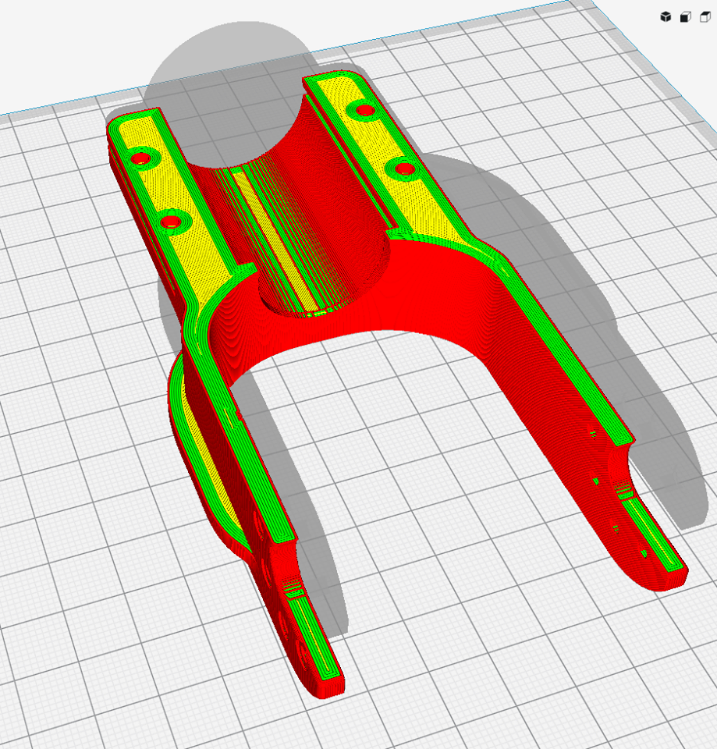
\includegraphics[width=\linewidth]{chapter4/images/fatigue3.png}
        \caption{รูปแสดงชั้นของการพิมพ์ตามแนวแกน x โดยการเติมเนื่อพลาสติก 100\%}
    \end{subfigure}
    \caption{รูปแสดงการแตกหักและชั้นการพิมพ์}
    \label{fig:fatiguelayer}
  \end{figure}

\subsubsection*{การทดลองความแข็งแรงของชิ้นงานโดยวิธีการวิเคราะห์เชิงตัวเลข(Finite element)}
ก่อนที่จะนำชิ้นงานที่ทำการออกแบบใหม่ที่เติมเนื่อพลาสติก 100\% ไปใช้งานจริงนั้นจะต้องผ่านการวิเคราะห์แรงกระทำ
โดยผ่านโปรแกรมจำลองเพื่อหาจุดที่เปราะบางของชิ้นงาน  และนำข้อมูลนั้นไปวิเคราะห์เพื่อปรับปรุงชิ้นงานต่อไป 
ซึ่งได้ตั้งค่า คุณสมบัติของชิ้นงานจากการพิมพ์สามมิติ ไว้ดังตารางที่ \ref{tab:PLA_property}

\begin{table}[!ht]
	\centering
	\begin{tabular}{| l | l |}
		\hline
		Print Orientation Side	& flat \\
        \hline
        Ultimate Stress $(N/mm²)$\footnote{Tensile Testing of 3D Printed Materials for Scoliosis Brace( Rahul Malik)} & 	45.66 \\
        Young’s Modulus $(N/mm²)$\footnote{Tensile Testing of 3D Printed Materials for Scoliosis Brace( Rahul Malik)} & 	1141.55 \\
        Yield strength $(N/mm²)$\footnote{What is the influence of infill \%, layer height and infill pattern on my 3D prints (3D Matter)} & 23 \\
        Density $(kg/m^3)$\footnote{Filament volume and length(toybuilderlabs)} &	1250 \\
        Passion ratio\footnote{Additive Manufacturing and Characterization of Polylactic Acid (PLA) Composites ContainingMetal Reinforcements(NASA)} &	0.33 \\
        Force (torque) $(N.m)$ & 10.4 \\
	    \hline
	\end{tabular}
	\caption{ตารางแสดงค่าคุณสมบัติของวัสดุจากเครื่องพิมพ์สามมิติ}
	\label{tab:PLA_property}
\end{table}
\vspace{-15pt}
เมื่อทดลองนำค่าดังกล่าวไปใช้ในโปรแกรม Solidwork และใช้ฟังก์ชัน Mass Property เพื่อหาค่าน้ำหนักที่ผ่านการคำนวณโดยโปรแกรม
และนำมาเทียบกับชิ้นงานจริงเพื่อดูว่ามีความคลาดเคลื่อนด้านน้ำหนักมากน้อยขนาดไหน พบว่าค่าข้อมูลความคลาดเคลื่อนนั้นจะไม่เกินกว่าระหว่าง $\pm 1\%$ กับค่าที่แสดงบนโปรแกรม
หลังจากนั้นทำการวิเคราะห์ผ่านโปรแกรม Solidwork ด้วยการวิเคราะห์ FEA ได้ผลลัพธ์ ดังนี้

\begin{figure}[!ht]
  \centering
  \begin{subfigure}[b]{0.32\linewidth}
    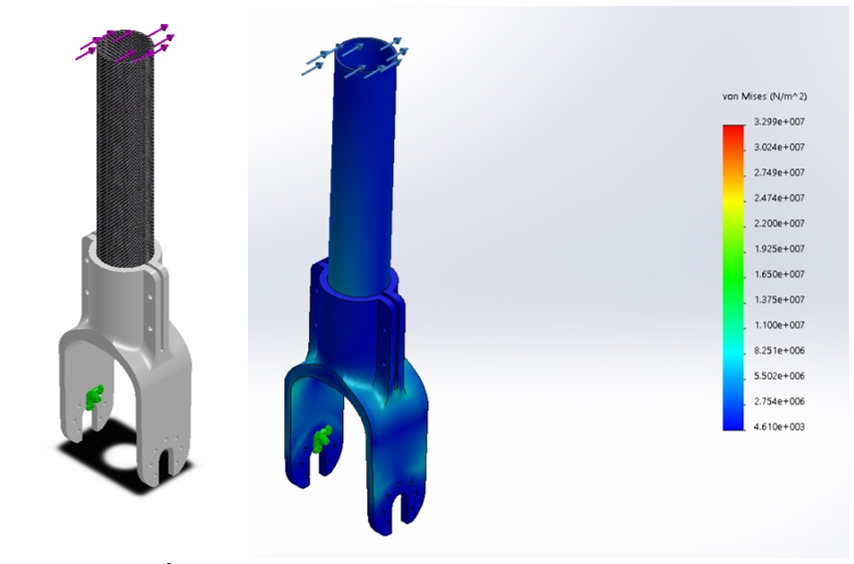
\includegraphics[width=\linewidth]{chapter4/images/FEA1.PNG}
    \caption{รูปการวิเคราะห์แรงของข้อต่อ 1}
  \end{subfigure}
  \begin{subfigure}[b]{0.32\linewidth}
    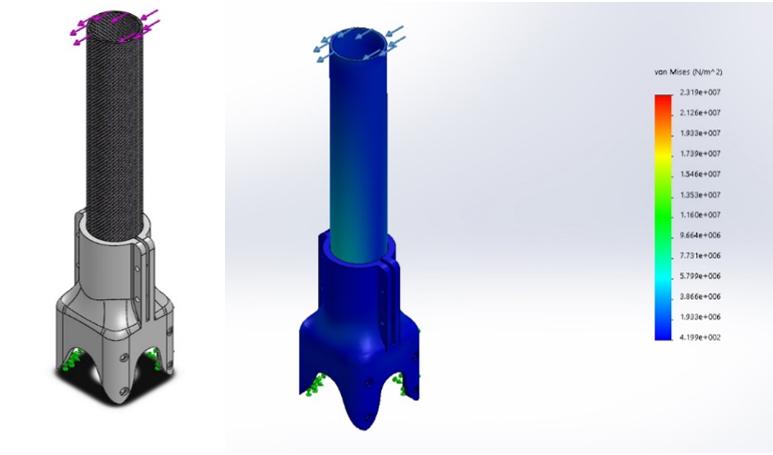
\includegraphics[width=\linewidth]{chapter4/images/FEA2.PNG}
    \caption{รูปการวิเคราะห์แรงของข้อต่อ 2}
  \end{subfigure}
  \begin{subfigure}[b]{0.32\linewidth}
      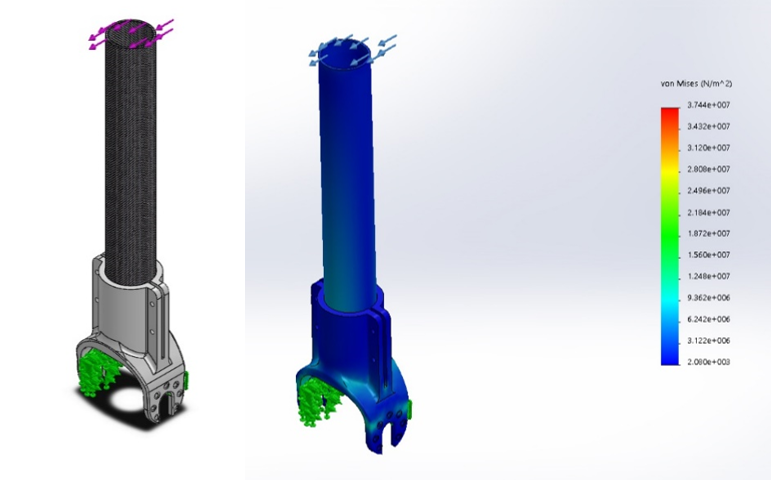
\includegraphics[width=\linewidth]{chapter4/images/FEA3.PNG}
      \caption{รูปการวิเคราะห์แรงของข้อต่อ 3}
  \end{subfigure}
  \caption{รูปการวิเคราะห์แรงของข้อต่อ}
\end{figure}
\vspace{-15pt}
การวิเคราะห์นั้นจะทำการยึดจุดที่เป็นหน้าแปลนของมอเตอร์ไว้เพื่อให้เปรียบเสมือนกับว่าขณะนี้ชิ้นงาน
ได้เชื่อมติดกับตัวมอเตอร์ หลังจากนั้นกำหนดแรงกระทำเพื่อให้เกิดโมเมนต์กับชิ้นงานโดยค่าแรงที่กระทำนั้น
ได้มาจากการคำณวนแรงของมอเตอร์ที่จะรับไหวเทียบกับระยะของแรง ที่กระทำกับชิ้นงาน 
ซึ่งได้ทดลองกับชิ้นงานตัวข้อต่อ 1 2 และ 3 ด้วยแรง 41.6 นิวตัน $(N)$
เมื่อนำค่า ความตึงเครียดสูงสุด $(Max stress)$ของชิ้นงานมาวิเคราะห์เพื่อหา จุดเปราะบางของวัสดุได้ค่าดังตาราง
\ref{tab:streaa_result}
\begin{table}[ht]
	\centering
	\begin{tabular}{| l | c |}
		\hline
		ชื่อชิ้นงาน	& ความตึงเครียดสูงสุดของชิ้นงาน(Max stress) $(N/mm^2)$ \\
        \hline
        ข้อต่อ 1 & 32.99 \\
        ข้อต่อ 2 & 23.19 \\
        ข้อต่อ 3 & 7.987 \\
	    \hline
	\end{tabular}
	\caption{ตารางแสดงความตึงเครียดของชิ้นงาน (Stress)}
	\label{tab:stress_result}
\end{table}
\vspace{-15pt}
จากผลการทดลองสรุปได้ว่า ค่าความตึงเครียดต่างๆที่ได้มาจากผลลัพธ์นั้นเมื่อนำไปเทียบกับค่าความตึงเครียดสูงสุดที่วัสดุจะรับไหว
ที่ 45.66 N/mm² เห็นได้ว่ายังคงไม่มีวัสดุตัวไหนที่จะเกิดการแตกหักเมื่อเกิดแรงกระทำกับชิ้นงานดังนั้นชิ้นงานที่ทำการออกแบบนี้
พอสรุปได้ว่าจะไม่เกิดการแตกหักระหว่างการทำงาน ยกแว้นมีแรงกระทำจากภายนอกที่มากเกินไปจนมาผลทำให้เกิดความตึงเครียดของชิ้นงานสูง
เกินกว่าค่าดังกล่าว  

\clearpage
\subsection{การออกแบบเท้า}
\subsubsection{การออกแบบโครงสร้างเท้าครั้งที่ 1}
โครงสร้างเท้านั้นได้ออกแบบให้มีลักษณะคล้ายคลึงกับรองเท้าของมนุษย์จริงและมีขนาดที่เหมาะสมกับตัวหุ่นยนต์ โดยคำนึงถึงความแข็งแรง
และการใช้งานเป็นหลัก และยังต้องขึ้นรูปด้วยเครื่องพิมพ์ 3 มิติได้อีกด้วย
\begin{figure}[!ht]
  \centering
  \begin{subfigure}[b]{0.55\linewidth}
    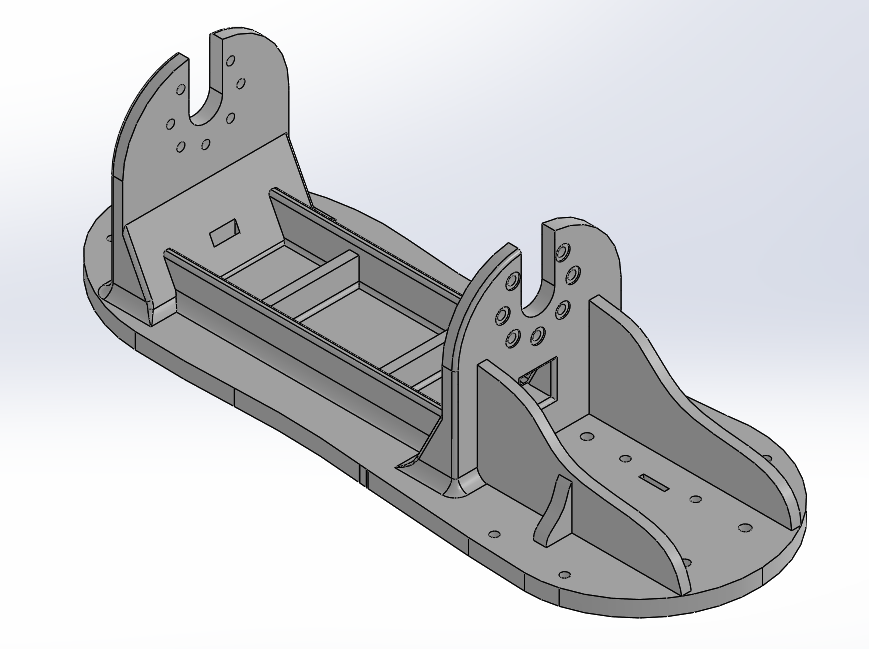
\includegraphics[width=\linewidth]{chapter4/images/foot_old.PNG}
    \caption{รูปแสดงเท้าของหุ่นยนต์}
  \end{subfigure}
  \begin{subfigure}[b]{0.2\linewidth}
    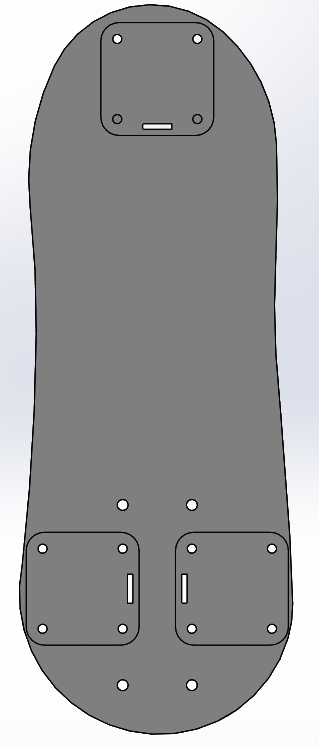
\includegraphics[width=\linewidth]{chapter4/images/bare_footold.PNG}
    \caption{รูปแสดงฝ่าเท้าของหุ่นยนต์}
  \end{subfigure}
  \caption{รูปแสดงเท้าของหุ่นยนต์ฮิวมานอยด์ UTHAI}
  \label{fig:footold}
\end{figure}

% \clearpage
ในส่วนของโครงครอบ FSR นั้นได้ออกแบบให้มีการกดโดยตรงกับหน้าสัมผัสซึ่งส่วนที่สัมผัสกับหน้าสัมผัสนั้นจะเป็นเฉพาะส่วนของ 3d print ที่ออกแบบมา
เฉพาะการกดโดยเฉพาะ ซึ่งจะทำให้ถนอมหน้าสัมผัสได้ดีกว่า การกดจากภายนอกโดยตรงซึ่งตัวเซนเซอร์นี้จะมีความสูงออกมาจากฝ่าเท่าเป็นระยะ 5.4 มิลลิเมตร 
โดยจะมีจำนวน 3 ตัวต่อเท้า 1 ข้าง
\begin{figure}[!ht]
  \centering
  \begin{subfigure}[b]{0.4\linewidth}
    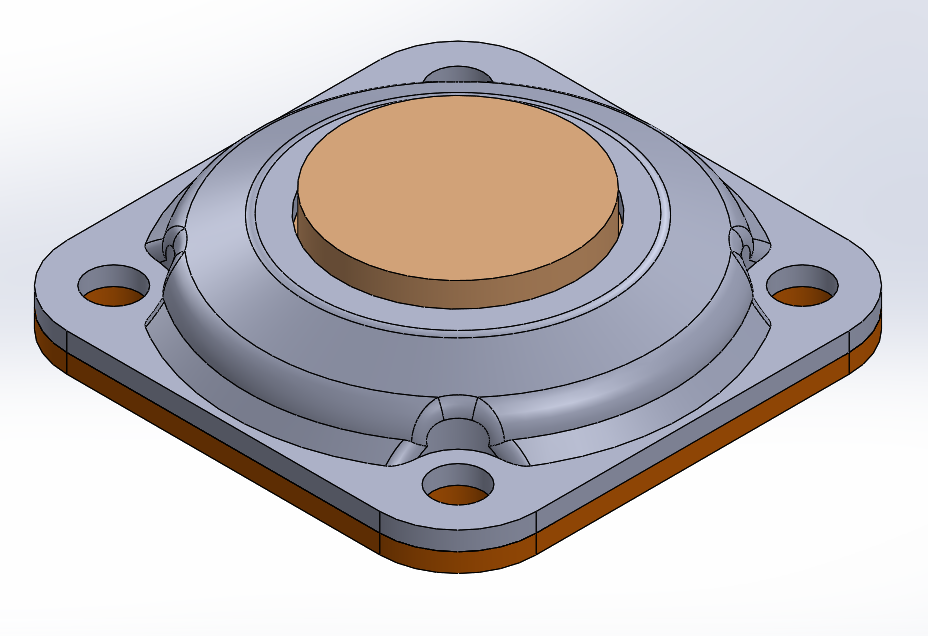
\includegraphics[width=\linewidth]{chapter4/images/FSR.PNG}
    \caption{รูปแสดงโครงครอบ FSR}
  \end{subfigure}
  \begin{subfigure}[b]{0.5\linewidth}
    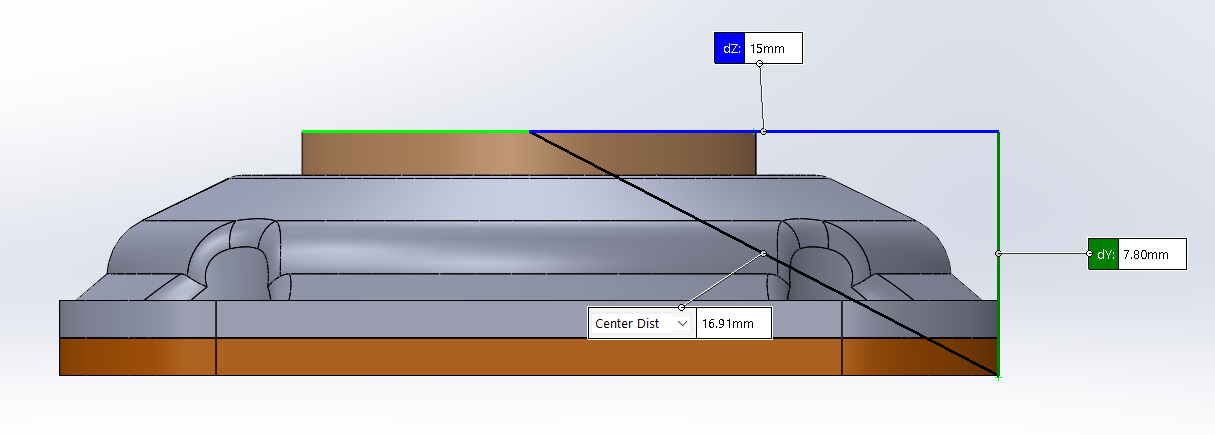
\includegraphics[width=\linewidth]{chapter4/images/FSR_mensure.PNG}
    \caption{รูปแสดงขนาดโครงครอบ FSR}
  \end{subfigure}
  \caption{รูปแสดงโดยรวมของโครงครอบ FSR}
  \label{fig:FSR}
\end{figure}

\clearpage
\subsubsection*{การทดลองความแข็งแรงของชิ้นงานโดยวิธีการวิเคราะห์เชิงตัวเลข (Finite element)}
จากค่าคุณสมบัติของชิ้นงานดังตาราง \ref{tab:PLA_property} นำมาวิเคราะห์ด้วยเทคนิคเชิงตัวเลขได้ผลดังนี้
\begin{figure}[!ht]
  \centering
  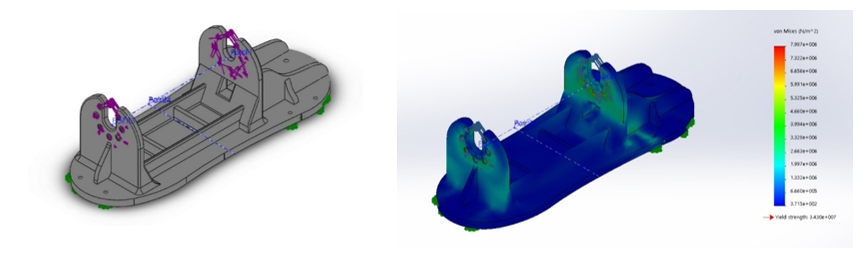
\includegraphics[width=0.9\textwidth]{chapter4/images/FEA4.PNG}
  \caption{รูปการวิเคราะห์แรงของเท้าหุ่นยนต์}
  \label{fig:FEA4}
\end{figure}
\vspace{-15pt}
การวิเคราะห์นั้นมีวิธีการทำเหมือนกับการวิเคราะห์ชิ้นส่วนขาคือทำการยึดจุดที่เป็นหน้าแปลนของดิจิตอลเซอร์โวไว้เพื่อให้เปรียบเสมือนกับว่าขณะนี้ชิ้นงานได้เชื่อมติดกับตัวดิจิตอลเซอร์โว
หลังจากนั้นกำหนดแรงกระทำเพื่อให้เกิดแรงบิดกับชิ้นงานโดยค่าแรงที่กระทำนั้นได้มาจากการคำณวนแรงของดิจิตอลเซอร์โวที่ทำกับชิ้นงานข้อเท้าที่แรงบิด 10.4 นิวตัน/เมตร $(N.m)$
ได้ผลดังตารางที่ \ref{tab:footstress_result}

\begin{table}[!ht]
	\centering
	\begin{tabular}{| l | c |}
		\hline
		ชื่อชิ้นงาน	& ความตึงเครียดสูงสุดของชิ้นงาน (Max stress) $(N/mm^2)$ \\
        \hline
        ฝ่าเท้า & 37.44 \\
	    \hline
	\end{tabular}
	\caption{ตารางแสดงความตึงเครียดของชิ้นงาน (Stress) ของฝ่าเท้า}
	\label{tab:footstress_result}
\end{table}
\vspace{-15pt}
% \clearpage
\subsubsection*{ปัญหาที่พบ}
เมื่อทำการประกอบชิ้นส่วนของ FSR กับฝ่าเท้าแล้วปัญหาที่พบคือ พื้นที่สัมผัสพื้นของฝ่าเท้า
น้อยลงซึ่งเป็นผลทำให้พื้นที่รองรับน้อยลงด้วยซึ่งเป็นเหตุทำให้การเดินของหุ่นยนต์นั้นยากลำบาก ดังนั้นจึงทำการแก้ไขโดย ออกแบบฝ่าเท้าให้มีขนาดใหญ่เพิ่มขึ้น และออกแบบเซนเซอร์ตรวจจับการเดินให้มีความบางลงอีกเพือให้หุ่นยนต์นั้น
มีพื้นที่รองรับเพิ่มขึ้น

\begin{figure}[!ht]
  \centering
  \begin{subfigure}[b]{0.2\linewidth}
    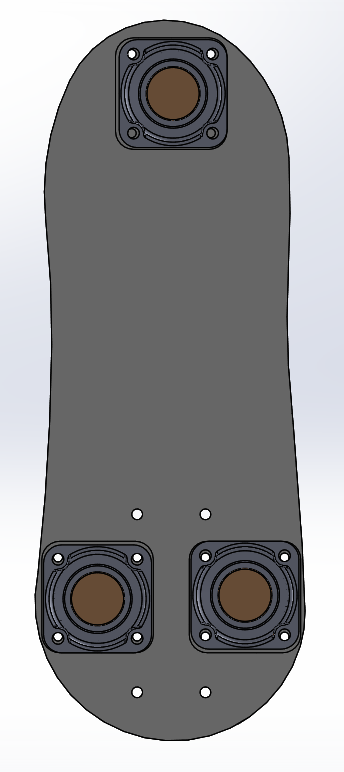
\includegraphics[width=\linewidth]{chapter4/images/foot+FSR.PNG}
    \caption{เท้าของหุ่นยนต์}
  \end{subfigure}
  \begin{subfigure}[b]{0.2\linewidth}
    \includegraphics[width=\linewidth]{chapter4/images/foot+FSR_sp.PNG}
    \caption{พื้นที่รองรับของเท้า}
  \end{subfigure}
  \caption{รูปแสดงฝ่าเท้าและพื้นที่รองรับ}
  \label{fig:foot_FSR}
\end{figure}



\clearpage
\subsubsection{การออกแบบโครงสร้างเท้าครั้งที่ 2}
ในการออกแบบครั้งนี้ได้เพิ่มขนาดของฝ่าเท้าให้ใหญ่ขึ้นเพื่อเพิ่มพื้นที่สัมผัสซึ่งจะเป็นผลทำให้หุ่นยนต์นั้นมีการเดินที่ง่ายขึ้น
ในการปรับขนาดครั้งนี้ได้เพิ่มขนาดที่ปลายเท้าให้ใหญ่ขึ้น และส้นเท้ารองลงมา
\begin{figure}[!ht]
  \centering
  \begin{subfigure}[b]{0.41\linewidth}
    \includegraphics[width=\linewidth]{chapter4/images/foot_new.PNG}
    \caption{รูปแสดงเท้าของหุ่นยนต์ที่ออกแบบใหม่}
  \end{subfigure}
  \begin{subfigure}[b]{0.4\linewidth}
    \includegraphics[width=\linewidth]{chapter4/images/foot_old.PNG}
    \caption{รูปแสดงเท้าของหุ่นยนต์เดิม}
  \end{subfigure}
  \begin{subfigure}[b]{0.2\linewidth}
    \includegraphics[width=\linewidth]{chapter4/images/bare_footnew.PNG}
    \caption{รูปแสดงฝ่าเท้าที่ออกแบบใหม่}
  \end{subfigure}
  \begin{subfigure}[b]{0.16\linewidth}
    \includegraphics[width=\linewidth]{chapter4/images/bare_footold.PNG}
    \caption{รูปแสดงฝ่าเท้าเดิม}
  \end{subfigure}
  \caption{รูปแสดงการเปรียบเทียบระหว่างเท้าเดิมและเท้าที่ออกแบบใหม่}
  \label{fig:foot_compilation}
\end{figure}

ในส่วนของเซนเซอร์ตรวจจับพื้นนั้นได้ทำการออกแบบใหม่ทั้งหมดให้มีความบางลงกว่าเดิม และให้มีส่วนที่ยื่นออกมา
จากฝ่าเท้าน้อยที่สุดซึ่งความสูงที่ยื่นออกมานั้นมีสความสูงเพียง 0.4 มิลลิเมตร ต่างจากเดิมที่มีความสูงถึง 5.4 มิลลิเมตร
\begin{figure}[!ht]
  \centering
  \begin{subfigure}[b]{0.25\linewidth}
    \includegraphics[width=\linewidth]{chapter4/images/FSR_new.PNG}
    \caption{รูปแสดงโครงครอบ FSR ที่ออกแบบใหม่}
  \end{subfigure}
  \begin{subfigure}[b]{0.25\linewidth}
    \includegraphics[width=\linewidth]{chapter4/images/FSR.PNG}
    \caption{รูปแสดงโครงครอบ FSR เดิม}
  \end{subfigure}
  \caption{รูปแสดงการเปรียบเทียบระหว่างฝ่าเท้าเดิมและฝ่าเท้าที่ออกแบบใหม่}
  \label{fig:barefoot_compilation}
\end{figure}

\clearpage
\subsubsection{ทดสอบการใช้งานของเซนเซอร์ตรวจจับการสัมผัสพื้น}
ในโครงงานนนี้เซนเซอร์ตรวจจับพื้นนั้นได้ใช้ใช้งานเพื่อตรวจการเหยียบของเท้าเท่านั้นว่ามีการแตะพื้นหรือไม่ ซึ่งจะกำหนดค่าไว้ในช่วง 
0-1023 โดยจะกำหนดให้ช่วงที่มากกว่า 1000 หมายถึงเท้ามีการยกเกิดขึ้นและต่ำกว่านั้นหมายถึงเท้ามีการเหยียบ โดยจะแปลงค่าเซนเซอร์ทั้ง 3 ค่าบนเท้า
เป็นค่าเฉลี่ยน้ำหนัก ตามสมการ $(sensor1 + sensor 2 + 2(sensor3))/4$ โดยให่ค่าตามแกน X เป็นค่า sampling(ครั้ง) ของข้อมูลและ
ค่าตามแกน Y เป็นค่าช่อง 0-1023 เมื่อทำการทดลองให้ทำการเหยียบเท้าและยกเท้าจะได้ผล ดังรูปที่ \ref{fig:FSR_graph}

\begin{figure}[!ht]
  \centering
  \includegraphics[width=0.6\textwidth]{chapter4/images/FSR_graph.PNG}
  \caption{รูปภาพแสดงค่าที่วัดได้ของ FSR}
  \label{fig:FSR_graph}
\end{figure}
ผลที่ได้นี้เกิดจากการทดลองยกเท้าของหุ่นยนต์ขึ้นขณะหุ่นยนต์ยืนอยู่และยกเท้าขึ้น ค่าที่อ่านได้จะมีค่า 1023 หรือสูงสุดตามภาพ และเมื่อเท้าสัมผัสพื้นนั้น
ค่าที่อ่านได้จะมีค่าที่ต่ำขึ้นอยู่กับแรงกดที่กระทำต่อเท้า ซึ่งถ้าค่าที่กระทำมากจะทำให้ค่าที่อ่านได้ต่ำมาก จะเห็นได้จากรูปภาพ \ref{fig:FSR_graph} 
จะมีช่วงเวลาหนึ่งที่ค่าที่อ่านได้ต่ำสุดซึ่งขณะนั้น ได้ทดลองกดด้วยแรงจำนวนหนึ่งที่มากกว่าน้ำหนักตัวหุ่นยนต์เป็นเวลา 1-2 วินาที


\clearpage
\subsection{การออกแบบโครงสร้างลำตัว}
ลำตัวของหุ่นยนต์นั้นจะใช้สำหรับติดตั้งหน่วยประมวลผลควบคุมระดับต่ำและระดับสูง IMU รวมไปถึงบอร์ดแปลงไฟ 12v จากแบตเตอรี่
ให้เหลือ 5V เพื่อจ่ายไฟให้กับระบบ ละยังคงต้องจัดเก็บแบตเตอรี่สำหรับทำงานไร้สายได้อีกด้วย 
\subsubsection{การออกแบบลำตัวครั้งที่ 1}
การออกแบบครั้งนี้ได้ออกแบบให้ลำตัวนั้นขึ้นรูปด้วยเครื่องพิมพ์ 3 มิติ เพื่อให้ง่ายสำหรับผู้ต่อยอดที่มีเครื่องพิมพ์เป็นของตนเอง สามารถพิมพ์
และนำมาประกอบได้ โดยส่วนของเอวนั้นจะใช้เป็นท่อคาร์บอนไฟเบอร์ขนาดเส้นผ่านศูนย์กลางขนาด 91 มิลลิเมตร เพื่อให้เหมาะสมกับชิ้นงาน
และเชื่อมยึดติดกันด้วยสกรูกับลำตัวและส่วนเอว
\begin{figure}[!ht]
  \centering
  \includegraphics[width=0.4\textwidth]{chapter4/images/troso_old.PNG}
  \caption{รูปภาพแสดงตัวของหุ่นยนต์ที่ออกแบบเพื่อขึ้นรูปด้วยเครื่องพิมพ์ 3 มิติ}
  \label{fig:torso_old}
\end{figure}

แต่เมื่อทำการทดลองหาค่ามวลในโปรแกรม solidwork แล้ว ได้ผลน้ำหนักคือ 711 กรัม ซึ่งเป็นน้ำหนักที่มากเกินไปอาจส่งผลทำให้
มอเตอร์รับน้ำหนักของตัวมากเกินไป ดังนั้นจึงเป็นผลทำให้ต้องเปลี่ยนการออกแบบให้เบาลงกว่าเดิม คือลดขนาดของตัวที่ขึ้นรูปด้วยเครื่องพิมพ์ 3 มิติ
ลงและใช้วัสดุผสมระหว่างคาร์บอนไฟเบอร์มากขึ้น ซึ่งจะยังคงได้ความแข็งแรงและความเบาอีกด้วย

\clearpage
\subsubsection{การออกแบบโครงสร้างตัวครั้งที่ 2}
จากปัญหาเรื่องน้ำหนักของชิ้นส่วนตัวของการออกแบบครั้งที่ 1 ได้แก้ไขโดยลดขนาดของส่วนพิมพ์ 3 มิติลงซึ่งจะแยกชิ้นส่วนออกเป็น 2 ส่วน คือส่วนหน้าและส่วนหลัง
และใช้การยึดกับท่อคาร์บอนไฟเบอร์ซึ่งเป็นส่วนเอวด้วยการบีบซึ่งทำโดยการร้อยสกรูผ่านช่องที่ทำไว้สำเร็จบนตัวชิ้นงานพิมพ์ 3 มิติ แล้วขันให้ชิ้นงานมาประกบเข้าหากัน
\begin{figure}[!ht]
  \centering
  \includegraphics[width=0.25\textwidth]{chapter4/images/troso_new.PNG}
  \caption{รูปภาพแสดงตัวของหุ่นยนต์ที่ออกแบบเพื่อขึ้นรูปด้วยเครื่องพิมพ์ 3 มิติ(ใหม่)}
  \label{fig:torso_new}
\end{figure}
ซึ่งน้ำหนักที่วิเคราะห์ได้โดยโปรแกรม solidwork นั้นได้ค่าเท่ากับ 342 กรัม ซึ่งน้อยกว่าการออกแบบครั้งแรกถึง 2 เท่า ซึ่งมีน้ำหนักมากถึง 711 กรัม

\subsubsection*{การยึดลำตัวกับสะโพก}
การยึดลำตัวกับสะโพกนั้นจะใช้รูปแบบการยึดโดยการถ่างวัสดุที่ทำขึ้นมาเพื่อยึดลำตัวกับสะโพกออกผ่านสกรู 1 ตัวที่ออกแบบไว้ โดยสกรูตัวนี้จะทำหน้าที่ดึงให้ถ้วยของตัวถ่าง
เคลื่อนที่ลงมาและในขณะนั้นเองตัวถ่างด้านนอกอีก 4 ตัว จะค่อยๆขยับออกถ่างให้มีแรงบีบกับขอบท่อคาร์บอนไฟเบอร์และยึดกันอย่างแน่นตรึง

\underline{ข้อแนะนำในการยึดให้แน่นมากขึ้น}
ควรจะใช้วัสดุที่มีความหนืด เช่น ยางในรถจักรยาน หรือแผ่นกันเลื่อน ยึดกับหน้าสัมผัสของตัวถ่างก่อนแล้วจึงนำไปยึดกับวัสดุจริง)


\begin{figure}[h!]
  \centering
  \begin{subfigure}[b]{0.4\linewidth}
    \includegraphics[width=\linewidth]{chapter4/images/hipconnector.PNG}
    \caption{รูปภาพแสดงอุปกรณ์ยึดระหว่างลำตัวกับสะโพก}
  \end{subfigure}
  \begin{subfigure}[b]{0.4\linewidth}
    \includegraphics[width=\linewidth]{chapter4/images/explode_hipconnect.PNG}
    \caption{รูปภาพแสดงการติดตั้งบนสะโพกพร้อมทำการยึดกับลำตัวหุ่นยนต์}
  \end{subfigure}
  \caption{รูปแสดงการใช้งานส่วนยึดสะโพกกับลำตัว}
  \label{fig:barefoot_compilation}
\end{figure}
\clearpage
\subsubsection*{การติดตั้งบอร์ดควบคุมและแบตเตอรี่}
เนื่องจากว่าบอร์ดควบคุมทั้ง 2 (Nucleo f411re,Odroid XU4)นั้นมีขนาดที่กระทัดรัด รวมถึงบอร์ด IMU และบอร์ดแปลงไฟ ที่มีขนาดเล็กเช่นกัน ฉะนั้นจึงได้ออกแบบ
ฐานสำหรับยึดบอร์ดทั้งหมดไว้ในที่เดียว และเมื่อติดตั้งในฐานเรียบร้อยแล้วก็สามารถนำฐานนั้น สวมลงไปในตัวของหุ่นยนต์ได้พอดี
\begin{figure}[!ht]
  \centering
  \includegraphics[width=0.4\textwidth]{chapter4/images/board_hold.PNG}
  \caption{รูปภาพแสดงฐานที่ติดตั้งบอร์ดควบคุม}
  \label{fig:board_hold}
\end{figure}
 

\begin{figure}[!ht]
  \centering
  \includegraphics[width=0.4\textwidth]{chapter4/images/install_board.PNG}
  \caption{รูปภาพแสดงตฐานที่ติดตั้งบอร์ดควบคุมในตัวของหุ่นยนต์}
  \label{fig:install_board}
\end{figure}

ซึ่งเมื่อทำการติดตั้งในตัวหุ่นยนต์แล้ว การยึดติดกับบอร์ดนั้นใช้หลักการยึดเดียวกับการยืดท่อคาร์บอนกับลำตัวคือ
ใช้แรงของการบีบอัดจากสกรูบนลำตัวทั้งหมด ยึดให้อยู่กับที่ ส่วนของแบตเตอรี่นั้นจะใช้เป็นแบตเตอรี่ขนาด 6000$mAh$ 12.6V
จะถูกติดตั้งในส่วนลำตัวของหุ่นยนต์บริเวณท่อคาร์บอนไฟเบอร์
\clearpage
\subsubsection{การออกแบบแขน}
แขนนั้นได้ออกแบบให้เรียบง่ายและน้ำหนักเบา ซึ่งในโครงงานนี้แขนจะเป็นหนึ่งในตัวแปรที่ช่วยในการเดินให้คล่องแคล่วมากขึ้น
โดยวัสดุหลักที่ใช้มาทำแขนนั้นจะมาจากวัสดุคาร์บอนไฟเบอร์เป็นหลักและชิ้นส่วนพิมพ์ 3 มิติจะใช้สำหรับเชื่อมวัสดุทั้งหมดเข้าด้วยกัน
\begin{figure}[h!]
  \centering
  \includegraphics[width=0.3\textwidth]{chapter4/images/troso.PNG}
  \caption{รูปภาพแสดงตัวของหุ่นยนต์ที่ติดตั้งแขนทั้ง 2 ข้าง}
  \label{fig:troso}
\end{figure}

% \subsection{น้ำหนักตัวหุ่นยนต์}
% หลังจากออกแบบและจัดทำชิ้นส่วนทั้งหมดเสร็จสมบูรณ์ ได้ทำการชั่งน้ำหนักของชิ้นส่วนทั้งหมดเพื่อหาน้ำหนักจริง
% เปรียบเทียบกับค่าที่ได้จากโปรแกรม solidwork ซึ่งผลที่ได้นี้จะเป็นน้ำหนักที่ยังไม่รวมน้ำหนักมอเตอร์ ทั้ง 14 ตัว
% และแบตเตอรี่ จะได้ผลดังตาราง
% \begin{table}[ht]
% 	\centering
% 	\begin{tabular}{| l | c | c |}
% 		\hline
% 		ชื่อชิ้นงาน	& น้ำหนักที่ชั่งจริง (กรัม) & น้ำหนักในโปรแกรม 3 มิติ (กรัม) \\
%         \hline
%         ลำตัว & & 342 \\
%         แขนซ้าย  & 272 & 241\\
%         แขนขวา  & 272 & 241\\
%         ต้นขา & 154 & 161 \\
%         หน้าแข้ง & 138 & \\
%         เท้า & & 148\\
% 	    \hline
% 	\end{tabular}
% 	\caption{ตารางแสดงความตึงเครียดของชิ้นงาน(Stress)}
% 	\label{tab:stress_result}
% \end{table}


% \clearpage
\subsection{แบบวาดทางวิศวกรรม}
\begin{figure}[h!]
  \centering
  \begin{subfigure}[b]{0.45\linewidth}
    \includegraphics[width=\linewidth]{chapter4/images/uthai_drawing_leg.png}
    \caption{ขาหุ่นยนต์ฮิวมานอยด์ UTHAI}
  \end{subfigure}
  \begin{subfigure}[b]{0.45\linewidth}
    \includegraphics[width=\linewidth]{chapter4/images/uthai_drawing_body.png}
    \caption{ตัวหุ่นยนต์ฮิวมานอยด์ UTHAI}
  \end{subfigure}
  \caption{ภาพแบบวาดทางวิศวกรรม}
  \label{fig:barefoot_compilation}
\end{figure}
% \begin{figure}[!ht]
%   \centering
%   \includegraphics[width=0.8\textwidth]{chapter4/images/uthai_drawing_leg.png}
%   \caption{ภาพแบบวาดทางวิศวกรรมของขาหุ่นยนต์ฮิวมานอยด์ UTHAI}
%   \label{fig:uthai_drawing_leg}
% \end{figure}
% \begin{figure}[!ht]
%   \centering
%   \includegraphics[width=0.8\textwidth]{chapter4/images/uthai_drawing_body.png}
%   \caption{ภาพแบบวาดทางวิศวกรรมของตัวหุ่นยนต์ฮิวมานอยด์ UTHAI}
%   \label{fig:uthai_drawing_body}
% \end{figure}

\clearpage
\section{การออกแบบโปรแกรมด้วย ROS}
\subsection{Simulation Gazebo}
ต้องติดตั้ง package ต่อไปนี้

% \begin{enumerate}[label=\arabic*, leftmargin=1.5cm]
% 	\item controller_manager\*
%     \item gazebo_ros_control\*
%     \item joint_state_controller
%     \item effort_controller
% \end{enumerate}

\begin{enumerate}[label=\arabic*, leftmargin=1.5cm]
	\item joint\_state\_controller
	\item effort\_controller
	\item controller\_manager*
	\item gazebo\_ros\_control*
\end{enumerate}

\clearpage
\section{การออกแบบระบบพื้นฐาน}
\subsection{GitHub ของหุ่นยนต์ฮิวมานอยด์ UTHAI}
ไฟล์ข้อมูลทุกอย่างเกี่ยวกับหุ่นยนต์ฮิวมานอยด์ UTHAIได้ถูกอัพโหลดขึ้นบนอินเทอร์เนต
โดยอัพโหลดไปไว้ที่ GitHub [https://github.com/UTHAI-Humanoid] และมีการเขียน Wiki การใช้งานเบื้องต้นเอาไว้
สำหรับนักศึกษาหรือนักวิจัยที่ต้องการพัฒนาต่อ 
\begin{figure}[!ht]
	\centering
	\includegraphics[width=0.42\textwidth]{chapter4/images/uthai_manual/uthai_github.png}
	\caption{GitHub ที่เก็บข้อมูลทั้งหมดของหุ่นยนต์ฮิวมานอยด์ UTHAI}
\end{figure}
\begin{figure}[!ht]
	\centering
	\includegraphics[width=0.60\textwidth]{chapter4/images/uthai_manual/uthai_github2.png}
	\caption{ตัวอย่าง Wiki การใช้งานเบื้องต้นของหุ่นยนต์ฮิวมานอยด์ UTHAI}
\end{figure}


\clearpage
\subsection{ตัวอย่างเฟรมของหุ่นยนต์ฮิวมานอยด์ UTHAI}
เฟรมของหุ่นยนต์ฮิวมานอยด์ UTHAIได้ถูกอัพโหลดให้อยู่บนอินเทอร์เน็ต โดยอยู่ที่ https://github.com/UTHAI-Humanoid/UTHAI-Hardware/tree/master/Mechanics/Frame

\begin{figure}[!ht]
	\centering
	\includegraphics[width=0.85\textwidth]{chapter4/images/uthai_manual/uthai_frame.png}
	\caption{ภาพเฟรมของแต่ละพาร์ทของหุ่นยนต์ฮิวมานอยด์ UTHAI}
\end{figure}
\begin{figure}[!ht]
	\centering
	\includegraphics[width=0.85\textwidth]{chapter4/images/uthai_manual/uthai_frame2.png}
	\caption{ภาพ GitHub ของเฟรมแต่ละพาร์ทของหุ่นยนต์ฮิวมานอยด์ UTHAI}
\end{figure}

\clearpage
\subsection{ตัวอย่างเอกสารข้อมูลของหุ่นยนต์ฮิวมานอยด์ UTHAI}

\begin{figure}[!ht]
    \centering
    \begin{subfigure}[b]{0.45\textwidth}
        \centering
        \includegraphics[width=\textwidth]{chapter4/images/uthai_manual/uthai_assembly.png}
        \caption{หน้าปกคู่มือการประกอบหุ่นยนต์ฮิวมานอยด์ UTHAI}
    \end{subfigure}
    \hfill
    \begin{subfigure}[b]{0.45\textwidth}
        \centering
        \includegraphics[width=\textwidth]{chapter4/images/uthai_manual/uthai_assembly2.png}
        \caption{ตัวอย่างคู่มือการประกอบหุ่นยนต์ฮิวมานอยด์ UTHAI}
    \end{subfigure}
    \caption{UTHAI Assembly Manual}
	\label{fig:uthai_assembly_manual}
\end{figure}
\begin{figure}[!ht]
    \centering
    \begin{subfigure}[b]{0.45\textwidth}
        \centering
        \includegraphics[width=\textwidth]{chapter4/images/uthai_manual/uthai_kinematics.png}
        \caption{หน้าปกรายละเอียดของหุ่นยนต์ฮิวมานอยด์ UTHAI}
    \end{subfigure}
    \hfill
    \begin{subfigure}[b]{0.45\textwidth}
        \centering
        \includegraphics[width=\textwidth]{chapter4/images/uthai_manual/uthai_kinematics2.png}
        \caption{ตัวอย่างรายละเอียดของหุ่นยนต์ฮิวมานอยด์ UTHAI}
    \end{subfigure}
    \caption{UTHAI Kinematics Properties}
	\label{fig:uthai_kinematics_manual}
\end{figure}
\begin{figure}[!ht]
    \centering
    \begin{subfigure}[b]{0.45\textwidth}
        \centering
        \includegraphics[width=\textwidth]{chapter4/images/uthai_manual/uthai_dynamics.png}
        \caption{หน้าปกรายละเอียดของหุ่นยนต์ฮิวมานอยด์ UTHAI}
    \end{subfigure}
    \hfill
    \begin{subfigure}[b]{0.45\textwidth}
        \centering
        \includegraphics[width=\textwidth]{chapter4/images/uthai_manual/uthai_dynamics2.png}
        \caption{ตัวอย่างรายละเอียดของหุ่นยนต์ฮิวมานอยด์ UTHAI}
    \end{subfigure}
    \caption{UTHAI Dynamics Properties}
	\label{fig:uthai_dynamics_manual}
\end{figure}


\clearpage
\subsection{ภาพรวมระบบพื้นฐานของหุ่นยนต์ฮิวมานอยด์ UTHAI}
ระบบพื้นฐานที่ผู้วิจัยได้ทำการออกแบบก็เพื่อที่จะทำให้คนที่เข้ามาพัฒนาต่อยอดได้อย่างสะดวก และเป็นระบบระเบียบ
มีรูปแบบแบบแผน ซึ่งผู้วิจัยได้วางระบบนี้ขึ้นมาจากประสบการณ์การทำงานของผู้วิจัยเอง รวมถึงได้ค้นคว้าหาความรู้เพิ่มเติม
จนคิดว่าระบบนี้จะทำให้หุ่นยนต์ฮิวมานอยด์สามารถพัฒนาต่อได้ง่าย และเป็นประโยชน์ต่อผู้วิจัยท่านอื่นที่ต้องการนำระบบพื้นฐานนี้ไปใช้งาน

\begin{figure}[!ht]
	\centering
	\includegraphics[width=0.7\textwidth]{chapter4/images/uthai_platform.png}
	\caption{ภาพรวมระบบพื้นฐานของหุ่นยนต์ฮิวมานอยด์ UTHAI}
	\label{fig:uthai_platform}
\end{figure}

ระบบพื้นฐานที่ผู้วิจัยออกแบบขึ้นมานั้น จะประกอบไปด้วยส่วนสำคัญอยู่ทั้งหมด 6 ส่วน คือ
\vspace{-10pt}
\begin{enumerate}[label=\arabic*., leftmargin=2.5cm]
    \setlength\itemsep{-0.25em}
    \item UTHAI-Documents
    \item UTHAI-Hardware
    \item UTHAI-Common
    \item UTHAI-MPPC
    \item UTHAI-OPC
    \item UTHAI-Tools
\end{enumerate}

\clearpage
\subsubsection*{UTHAI-Documents}
ในส่วนนี้คือส่วนของงานเอกสารต่างๆที่เกี่ยวข้องกับหุ่นยนต์ฮิวมานอยด์

\paragraph*{Reports-Hardware}
ใช้สำหรับเก็บรายงานวิทยานิพนธ์ทั้งฉบับร่างและฉบับสมบูรณ์ที่เกี่ยวข้องกับ การปรับเปลี่ยนโครงสร้างทางกล และทางไฟฟ้าของหุ่นยนต์ฮิวมานอยด์ UTHAI
\subparagraph*{- การออกแบบโครงสร้างและพัฒนาระบบพื้นฐานสำหรับหุ่นยนต์ฮิวมานอยด์เพื่อการศึกษาและวิจัย}

\paragraph*{Reports-Software}
ใช้สำหรับเก็บรายงานวิทยานิพนธ์ทั้งฉบับร่างและฉบับสมบูรณ์ที่เกี่ยวข้องกับการเพิ่มความสามารถของหุ่นยนต์ฮิวมานอยด์ UTHAI
\subparagraph*{- การพัฒนาระบบการเคลื่อนที่สำหรับหุ่นยนต์ฮิวมานอยด์}

\paragraph*{Wiki}
ใช้สำหรับเก็บ Tutorial ที่เกี่ยวกับการใช้งานของหุ่นยนต์ฮิวมานอยด์ UTHAI

\begin{figure}[!ht]
	\centering
	\includegraphics[width=0.7\textwidth]{chapter4/images/uthai_platform/uthai_doc.png}
	\caption{ภาพตัวอย่าง Tutorial ใน Wiki}
\end{figure}

ผู้วิจัยท่านอื่นสามารถที่จะช่วยกันเขียนและพัฒนาได้โดยการ Clone Repository แล้วทำการแก้ไขปรับปรุง หลังจากนั้นก็ Pull request ขึ้นมาเพื่อแสดงให้ผู้วิจัยท่านอื่นเห็นด้วย


\clearpage
\subsubsection*{UTHAI-Hardware}
ในส่วนนี้คือส่วนของรายละเอียดเกี่ยวกับโครงสร้างทั้งทางกลและทางไฟฟ้าที่เปิดให้ผู้วิจัยท่านอื่นสามารถนำไปประยุกต์ใช้ได้

\paragraph*{Drawing}
ไฟล์ออกแบบทางวิศวกรรมทุกชิ้นส่วนที่ต้องมีการขึ้นรูป
\paragraph*{STL files}
ไฟล์สำหรับการขึ้นรูปสามมิติและไฟล์สำหรับนำไปทำแบบจำลองหุ่นยนต์ฮิวมานอยด์
\paragraph*{Solidworks files}
ไฟล์ที่ออกแบบโดยใช้โปรแกรม Solidworks เพื่อให้นำไปแก้ไขปรับปรุงให้ดียิ่งขึ้นได้

\begin{figure}[!ht]
	\centering
	\includegraphics[width=0.8\textwidth]{chapter4/images/uthai_platform/uthai_hardware1.png}
	\caption{ภาพตัวอย่างไฟล์ใน UTHAI-Hardware}
\end{figure}
\begin{figure}[!ht]
	\centering
	\includegraphics[width=0.8\textwidth]{chapter4/images/uthai_platform/uthai_properties.png}
	\caption{ภาพตัวอย่างไฟล์ใน UTHAI-Hardware}
\end{figure}


\clearpage
\subsubsection*{UTHAI-Common}
ในส่วนนี้คือส่วนของแพกเกจ ROS ที่ใช้เป็นพื้นฐานสำหรับการแสดงผลด้วยภาพ และระบบจำลองโดยจะมีแบบจำลองของหุ่นยนต์ฮิวมานอยด์ UTHAI ในรูปแบบของ URDF Xacro
\paragraph*{uthai\_description}
เป็นแพกเกจที่เขียนอธิบายลักษณะของหุ่นยนต์ฮิวมานอยด์เพื่อให้ ROS สามารถนำไปใช้ในกระบวนการอื่นได้
\paragraph*{uthai\_gazebo}
เป็นแพกเกจที่เอาไว้สำหรับทำระบบจำลองการทำงานของหุ่นยนต์ฮิวมานอยด์ UTHAI

\begin{figure}[!ht]
	\centering
	\includegraphics[width=0.6\textwidth]{chapter4/images/uthai_platform/uthai_rviz.png}
	\caption{ภาพ RViz ใน uthao\_description}
\end{figure}
\begin{figure}[!ht]
	\centering
	\includegraphics[width=0.6\textwidth]{chapter4/images/uthai_platform/uthai_gazebo.png}
	\caption{ภาพ Gazebo ใน uthai\_gazebo}
\end{figure}


\clearpage
\subsubsection*{UTHAI-MPPC}
ในส่วนนี้คือส่วนของแพกเกจ ROS ที่ใช้เป็นตัวในการเชื่อมต่อกับอุปกรณ์ฮาร์ดแวร์ของหุ่นยนต์ฮิวมานอยด์ UTHAI
เพื่อสั่งการตัวขับเคลื่อนดิจิตอลเซอร์โว และอ่านค่าเซนเซอร์จากตัวรับรู้หน่วยวัดความเฉื่อย การตรวจจับฝ่าเท้า
ตำแหน่งและความเร็วของตัวขับเคลื่อน
\paragraph*{uthai\_mbed}
เป็นแพกเกจที่เขียนเชื่อมต่อกับหน่วยประมวลผลระดับต่ำผ่าน rosserial เขียนด้วยภาษา python
โดยจะรับค่าเซนเซอร์หน่วยวัดความเฉื่อย เซนเซอร์ตรวจจับพื้น
\paragraph*{uthai\_manager}
เป็นแพกเกจที่เขียนเพื่อเอาไว้สำหรับจัดการตัวขับเคลื่อนทั้งหมด ให้สามารถสั่งการได้รวมถึง config ต่างๆด้วย
\paragraph*{uthai\_bringup}
เป็นแพกเกจที่เขียนเพื่อใช้ในการสั่งการตัวขับเคลื่อน ดิจิตอลเซอร์โว ที่เชื่อมต่อกับตัวประมวลผลระดับสูง

\begin{figure}[!ht]
	\centering
	\includegraphics[width=0.8\textwidth]{chapter4/images/uthai_platform/ros_serial.png}
	\caption{ภาพ rqt\_graph ของ serial\_node}
\end{figure}


\subsubsection*{UTHAI-OPC}
ในส่วนนี้คือส่วนของแพกเกจ ROS ที่ใช้เป็นตัวในการเชื่อมต่อระหว่างตัวประมวลผลระดับสูงกับคอมพิวเตอร์ภายนอกเพื่อใช้ในการควบคุม
หรือการแสดงผลการทำงานที่ต้องใช้การคำนวณสูง เป็นการแบ่งเบาภาระการประมวลผลของตัวประมวลผลระดับสูง

\subsubsection*{UTHAI-Msgs}
ในส่วนนี้คือส่วนของแพกเกจ ROS ที่ใช้เป็นตัวในการเก็บ Messages ที่ใช้ในการติดต่อสื่อสารกันภายในระบบ ซึ่ง Messages ไม่เป็นมาตรฐาน
โดยอาจรวมไปถึง services และ actions ของระบบหุ่นยนต์ฮิวมานอยด์ UTHAIด้วย

\clearpage
\subsubsection*{UTHAI-Tools}
ในส่วนนี้คือส่วนของรายละเอียดเเครื่องมือที่ช่วยทำให้การทำงานมีประสิทธิภาพมากยิ่งขึ้น

\paragraph*{sketch-lib}
เป็นเครื่องมือที่ใช้สำหรับเอาไว้วาดรูปเฟรมของหุ่นยนต์
\begin{figure}[!ht]
    \centering
    \begin{subfigure}[b]{0.45\textwidth}
        \centering
        \includegraphics[width=\textwidth]{chapter4/images/uthai_tools/basic-shapes.png}
        \caption{ภาพตัวอย่างการวาดออฟเจ็คต่างๆ}
    \end{subfigure}
    \hfill
    \begin{subfigure}[b]{0.45\textwidth}
        \centering
        \includegraphics[width=\textwidth]{chapter4/images/uthai_tools/test_robot.png}
        \caption{ภาพตัวอย่างการวาดเฟรมของแขนกล}
    \end{subfigure}
    \caption{ภาพตัวอย่างการวาดเฟรมโดยใช้เครื่องมือนี้}
\end{figure}
\begin{figure}[!ht]
	\centering
	\includegraphics[width=0.3\textwidth]{chapter4/images/uthai_tools/uthai_kinematics.png}
	\caption{ภาพตัวอย่างการวาดเฟรมของหุ่นยนต์ฮิวมานอยด์}
	\label{fig:uthai_kinematics_sk}
\end{figure}

\clearpage
\section{ผลการทดลอง}
\subsection{การทดลองการเดิน}
การทดลองการเดินนั้นได้ทดลองด้วยการปรับค่าข้อต่อให้เหมาะสมแก่การเดิน เพื่อทดสอบโครงสร้างที่ได้ออกแบบ
มาว่าสามารถรองรับการเดินของหุ่นยนต์ได้จริงหรือไม่ โดยค่าที่ใช้ในการปรับนั้นจะเป็นค่ามุมของมอเตอร์ส่วนต่างๆของส่วนขาทั้ง 2 ข้าง
โดยจะตั้งชื่อมอเตอร์ตามแกนของข้อต่อแต่ละส่วนโดยเริ่มจากส่วนจะโพกจะมี 3 แกนคือ hip yaw,hip roll,hip pitch ส่วนหัวเข่า 1 แกนคือ
knee pitch และส่วนข้อเท้า 2 แกนคือ ankle pitch,ankle roll โดยในขาแต่ละข้างจะแยกด้วยสัญลักษณ์ Right(ขาข้างขวา)และ Left(ขาข้างซ้าย)
โดยอิงจากตัวของหุ่นยนต์ และสั่งงานให้ไปตามมุมต่างๆที่กำหนดไว้ดังภาพ 

\subsubsection*{รูปกราฟแสดงตำแหน่งมอเตอร์ขาขวา}
\begin{figure}[!ht]
  \centering
  \includegraphics[width=1.0\linewidth]{chapter4/images/right_hip_roll.png}
  \caption{รูปการสั่งงานข้อต่อ right hip roll}
  \label{fig:right_hip_roll}
\end{figure}
\clearpage

\begin{figure}[!ht]
  \centering
  \includegraphics[width=1.0\linewidth]{chapter4/images/right_hip_pitch.png}
  \caption{รูปการสั่งงานข้อต่อ right hip pitch}
  \label{fig:right_hip_pitch}
\end{figure}

\begin{figure}[!ht]
  \centering
  \includegraphics[width=1.0\linewidth]{chapter4/images/right_hip_yaw.png}
  \caption{รูปการสั่งงานข้อต่อ right hip yaw}
  \label{fig:right_hip_yaw}
\end{figure}
\clearpage

\begin{figure}[!ht]
  \centering
  \includegraphics[width=1.0\linewidth]{chapter4/images/right_knee_pitch.png}
  \caption{รูปการสั่งงานข้อต่อ right knee pitch}
  \label{fig:right_knee_pitch}
\end{figure}

\begin{figure}[!ht]
  \centering
  \includegraphics[width=1.0\linewidth]{chapter4/images/right_ankle_pitch.png}
  \caption{รูปการสั่งงานข้อต่อ right ankle pitch}
  \label{fig:right_ankle_pitch}
\end{figure}
\clearpage

\begin{figure}[!ht]
  \centering
  \includegraphics[width=1.0\linewidth]{chapter4/images/right_ankle_roll.png}
  \caption{รูปการสั่งงานข้อต่อ right ankle roll}
  \label{fig:right_ankle_roll}
\end{figure} 
\clearpage
  
\subsubsection*{รูปกราฟแสดงตำแหน่งมอเตอร์ขาซ้าย}
\begin{figure}[!ht]
  \centering
  \includegraphics[width=1.0\linewidth]{chapter4/images/left_hip_roll.png}
  \caption{รูปการสั่งงานข้อต่อ left hip roll}
  \label{fig:left_hip_roll}
\end{figure}

\begin{figure}[!ht]
  \centering
  \includegraphics[width=1.0\linewidth]{chapter4/images/left_hip_pitch.png}
  \caption{รูปการสั่งงานข้อต่อ left hip pitch}
  \label{fig:left_hip_pitch}
\end{figure}
\clearpage

\begin{figure}[!ht]
  \centering
  \includegraphics[width=1.0\linewidth]{chapter4/images/left_hip_yaw.png}
  \caption{รูปการสั่งงานข้อต่อ left hip yaw}
  \label{fig:left_hip_yaw}
\end{figure}

\begin{figure}[!ht]
  \centering
  \includegraphics[width=1.0\linewidth]{chapter4/images/left_knee_pitch.png}
  \caption{รูปการสั่งงานข้อต่อ left knee pitch}
  \label{fig:left_knee_pitch}
\end{figure}
\clearpage

\begin{figure}[!ht]
  \centering
  \includegraphics[width=1.0\linewidth]{chapter4/images/left_ankle_pitch.png}
  \caption{รูปการสั่งงานข้อต่อ left ankle pitch}
  \label{fig:left_ankle_pitch}
\end{figure}

\begin{figure}[!ht]
  \centering
  \includegraphics[width=1.0\linewidth]{chapter4/images/left_ankle_roll.png}
  \caption{รูปการสั่งงานข้อต่อ left ankle roll}
  \label{fig:left_ankle_roll}
\end{figure} 
\clearpage

จากกราฟที่แสดงข้างต้นนั้นแสดงถึงตำแหน่งที่สั่งงานให้หุ่นยนต์ขยับในองศาต่างๆของข้อต่อ โดยจะสามารถสังเกตได้จาก
จุด peak ของแต่ละกราฟซึ่งมี 7 จุดในแต่ละกราฟที่เกิดขึ้นในคาบที่ไกล้เคียงกัน โดยค่าในแกน x แสดงถึงช่วงเวลาที่สั่งงานเป็นวินาที 
และแกน y แสดงองศาของมอเตอร์ในหน่วยเรเดียล โดยในการทดลองนี้ เป็นการกำหนดค่าเพื่อทดลองให้หุ่นยนต์มีการเดินเกิดขึ้น
และทดสอบโครงสร้างขณะทำการทดลองอีกด้วย ซึ่งผลการทดลองที่ได้จะพบว่าการเดินครั้งที่ 1-4 เกิดการล้มขึ้น และหลังจากครั้งที่ 5 เป็นต้นไป
หุ่นยนต์สามารถเดินได้ 1 ก้าวจากการทดลองเปลี่ยนค่าให้เหมาะสมกับระบบ ดังแสดงในรูปภาพต่อไปนี้

\begin{figure}[!ht]
    \centering
    \begin{subfigure}[b]{0.4\linewidth}
      \includegraphics[width=\linewidth]{chapter4/images/fall1.png}
      \caption{รูปการล้มครั้งที่ 1}
    \end{subfigure}
    \begin{subfigure}[b]{0.4\linewidth}
      \includegraphics[width=\linewidth]{chapter4/images/fall2.png}
      \caption{รูปการล้มครั้งที่ 2}
    \end{subfigure}
    \begin{subfigure}[b]{0.4\linewidth}
      \includegraphics[width=\linewidth]{chapter4/images/fall3.png}
      \caption{รูปการล้มครั้งที่ 3}
    \end{subfigure}
    \begin{subfigure}[b]{0.4\linewidth}
      \includegraphics[width=\linewidth]{chapter4/images/fall4.png}
      \caption{รูปการล้มครั้งที่ 4}
    \end{subfigure}
    \begin{subfigure}[b]{0.4\linewidth}
      \includegraphics[width=\linewidth]{chapter4/images/achive1.png}
      \caption{รูปการก้าวสำเร็จ}
    \end{subfigure}
    \caption{รูปการทดลองการเดินของหุ่นยนต์ UTHAI}
    \label{fig:test_result}
  \end{figure}


\clearpage
\subsection{ปัญหาที่พบและการแก้ไข}
\subsubsection{อุณหภูมิ}
เมื่อมีการใช้งานเป็นเวลานานจะส่งผลให้มอเตอร์ส่วนสะโพกและข้อเท้ามีความร้อนสูงถึง 50 องศาเซลเซียส 
เนื่องจากมีการสั่งงานให้มอเตอร์อยู่ในตำแหน่งที่กำหนด ซึ่งเมื่อมีแรงบิดข้างนอกมาเกี่ยวข้อง จะทำให้มอเตอร์นั้น
พยายามรักษามุมของตนเองไว้ ส่งผลให้เกิดความร้อนเกิดขึ้นและ ส่งผลให้มอเตอร์อ่อนแรงลงเนื่องจากความร้อนที่เกิดขึ้น 
ในการแก้ไขปัญหานี้สามารถเพิ่มเติมส่วนของการระบายอากาศซึ่งจะส่งผลให้ตัวของหุ่นยนต์นั้นมีน้ำหนักมากขึ้น หรือ หยุดการทดลอง
ไว้สักระยะเพื่อให้มีการระบายอากาศให้อยู่ในอุณหภูมิปกติ
\subsubsection{โครงสร้าง}
เนื่องจากการยึดท่อคาร์บอนไฟเบอร์นั้นได้ทำการยึดด้วยการบีบอัดเพื่อให้เกิดแรงเสียดทางสูงแต่ว่าเมื่อมีการ สั่งงานที่มีการกระชากกล่าวคือ
มีการเคลื่อนที่ของมุมมอเตอร์ที่มีความแร็วสูง จะส่งผลให้เกิดแรงบิดตามแนวแกนซึ่งเกินแรงเสียดทานที่การยึดติดจะรับไหว จึงเกิดการบิด ของข้อต่อ
เกิดขึ้น ส่งผลให้ ส่วนของเท้ามีการบิดไปจากท่าปกติ ซึ่งสามารถแก้ไขได้โดยเพิ่มแรงยึดด้วยการเสริมแผ่นยางบางๆบริเวณหน้าสัมผัสที่ติดกับท่อคาร์บอนไฟเบอร์
เพื่อเพิ่มแรงยึดไปอีกขั้นหนึ่ง 
\subsubsection{มอเตอร์}
เนื่องจากว่าตัวหุ่นยนต์มีการใช้มอเตอร์ในการขับเคลื่อนโดยตรงกับข้อต่อ ซึ่งเป็นผลทำให้ต้องใช้มอเตอร์ที่มีแรงบิดสูง
เพื่อขับเคลื่อนให้โครงสร้างมีการขยับตัวได้ แต่เนื่องจากว่าตัวหุ่นยนต์นั้นออกแบบมาให้มีความสูงที่ระดับ 1 เมตร ซึ่งหมายถึงจะมีแรง
โมเมนต์ที่เกิดขึ้นกับข้อต่อเมื่อหุ่นยนต์มีการก้าวเท้าหรือขยับตัว เป็นผลทำให้เกิด backlash เนื่องจากว่าตัวของมอเตอร์เองไม่สามารถควบคุมตำแหน่งของตนเองให้อยู่
ในมุมที่สั้งงานไว้ได้ จึงแก้ไขปัญหาโดยการเพิ่มระยะการสั่งงานเพื่อให้ครอบคลุมช่วง blacklash เพื่อที่จะให้ไปยังมุมที่ต้องการได้ และยังเพิ่มกำลังไฟให้กับมอเตอร์
จาก 12V เป็น 14V เพื่อให้มีแรงบิดที่เพิ่มมากขึ้นกว่าเดิม ซึ่งจะส่งให้ backlash น้อยลงและสามารถคุมตำแหน่งงายขึ้น



% % ************************** Thesis Chapter5 **********************************

\chapter{สรุปผลการทดลองและข้อเสนอแนะ}

\section{การออกแบบโครงสร้างของหุ่นยนต์}
การออกแบบโครงสร้างหุ่นยนต์ฮิวมานอยด์ UTHAI มุ่งเน้น 2 ส่วนเป็นหลักคือ
\vspace{-3mm}
\begin{enumerate}[label=\arabic*, leftmargin=1.5cm]
	\setlength\itemsep{-0.25em}
	\item สามารถสร้างขึ้นได้ง่าย
	\item น้ำหนักเบา
\end{enumerate}

ผู้วิจัยจึงเลือกที่จะประยุกต์ใช้เทคนิคการพิมพ์ขึ้นรูปสามมิติด้วยเครื่องพิมพ์สามมิติ ในการขึ้นรูปข้อต่อส่วนต่างๆของหุ่นยนต์ฮิวมานอยด์อุทัย
และก้านต่อได้เลือกใช้วัสดุเป็นคาร์บอนไฟเบอร์ ซึ่งเป็นวัสดุที่มีคุณสมบัติคือ เบา และแข็งแรง เมื่อเทียบกับวัสดุอื่นๆ ทำให้หุ่นยนต์ฮิวมานอยด์อุทัยมีน้ำหนักเบา
การเชื่อมต่อระหว่างข้อต่อ กับก้านต่อคาร์บอนไฟเบอร์ ผู้วัจัยใช้วิธีการบีบเพื่อสร้างแรงเสียดทานในการยึดติด
เนื่องจากการเจาะท่อคาร์บอนไฟเบอร์จะทำให้ใยไฟเบอร์ขาด ซึ่งส่งผลต่อความแข็งแรงของท่อคาร์บอนไฟเบอร์เป็นอย่างมาก
อีกทั้งเมื่อมีการเคลื่อนไหวและรับแรงในแนวต่างๆจะทำให้รูที่เจาะขยายและคลอนได้ส่งผลต่อความแม่นยำโดยรวมของหุ่นยนต์
แต่การยึดติดด้วยวิธีการบีบกับท่อคาร์บอนไฟเบอร์นั้นมีปัญหาเกิดขึ้นคือ มีโอกาสที่จะประกอบโครงสร้างของหุ่นยนต์ไม่ตรงเพราะอาจเกิดการหมุนตามแนวยาวของชิ้นส่วน
และหากใช้งานต่อเนื่องจะทำให้เกิดการหมุนเลื่อนตามแนวยาวของท่อได้ แต่มีข้อดีคือ เมื่อมีการบิดตามแนวแกนของท่อคาร์บอนเกิดขึ้นแทนที่ชิ้นส่วนจะเกิดการแตกหักเนื่องจาก 
แรกบิดนั้น ตรงส่วนที่ทำการยึดด้วยการบีบอัดนั้นจะเป็นตัวกลางรับแรงบิดแทน ส่งผลให้การยึดมีการบิดเปลี่ยนรูปตามแนวยาวของท่อ แต่ก็สามารถบิดกลับมาให้คงรูปเดิมได้

ส่วนของการเดินของหุ่นยนต์นั้นได้พบว่าเมื่อหุ่นยนต์มีการเดินจริงจะมี backlash เกิดขึ้นในส่วนของตัวมอเตอร์และชุดเฟือง และการเปลี่ยนรูปร่าง
ของข้อต่อที่เชื่อมกับมอเตอร์ ซึ่งทำให้การทดสอบเดินนั้นเป็นไปได้อย่างยากลำบาก โดยจะต้องเผื่อค่าเพื่อให้หุ่นยนต์เข้าที่ตามท่าทางที่กำหนด  

\subsection*{ข้อเสนอแนะ}

การพัฒนาต่อยอดควรปรับปรุงในส่วนการเชื่อมต่อเข้าด้วยกันระหว่างมอเตอร์และก้านต่อ ซึ่งอาจจะเพิ่มด้วยวิธีเพิ่มรอยบากเพื่อให้ศูนย์ของมอเตอร์ตรงกัน
และการประกอบโครงสร้างควรใช้วัสดุแผ่นยางบางมาคั่นกลางระหว่างหน้าสัมผัสที่ท่อคาร์บอนไฟเบอร์ซึ่งแผ่นยางจะสัมผัสกับชิ้นส่วนที่พิมพ์จากเครื่องพิมพ์สามมิติทำให้มีแรงยึดเกาะ
เพิ่มมากขึ้น

ส่วนของมอเตอร์ เนื่องจากว่าหุ่นยนต์ที่ออกแบบนี้มีการออกแบบให้มีความสูง 1 เมตร ซึ่งทำให้ส่วนขาของหุ่นยนต์มีความยาวที่มาก เป็นผลทำให้
สามารถเกิดโมเมนต์เมื่อกระทำการเดิน จึงส่งผลทำให้หุ่นยนต์เกิด backlash ที่ตัวของมอเตอร์เองเพราะเนื่องจากตัวของมอเตอร์ไม่สามารถควบคุม
ตำแหน่งของตนให้อยู่ในตำแหน่งที่สั่งการไปได้ ในการแก้ไขนี้สามารถแก้ไขได้โดย การลดขนาดความยาวของขาลงเพื่อให้เกิดโมเมนต์ที่มอเตอร์ส่วนสะโพกที่น้อยกว่าเดิม
หรือเปลี่ยนมอเตอร์ให้สามารถรับแรงบิดที่สูงกว่าตัวปัจจุบัน เพราะสามารถคงสภาพมุมที่สั่งการได้อย่างแม่นยำและเกิด backlash น้อยกว่าตัวปัจจุบันได้มาก
และสามารถแก้ไขเรื่องอุณหภูิที่เกิดขึ้นเมื่อมีการใช้งานเป็นเวลานาน ซึ่งตัวมอเตอร์ปัจจุบันเมื่อมีการใช้งานสักระยะหนึ่ง มอเตอร์จะเกิดการอ่อนแรง เนื่องจากความร้อน



\clearpage
\section{การออกแบบโปรแกรมด้วย ROS}
การออกแบบโปรแกรมของหุ่นยนต์ฮิวมานอยด์ UTHAI ผู้วิจัยได้ใช้ ROS เป็นเครื่องมือที่ช่วยในการทำงาน
ในวิทยานิพนธ์นี้ส่วนของโปรแกรมจะแบ่งออกเป็น 3 ส่วนหลักคือ
\vspace{-3mm}
\begin{enumerate}[label=\arabic*, leftmargin=1.5cm]
	\setlength\itemsep{-0.25em}
	\item การแสดงผลภาพด้วย RViz
    \item การจำลองการทำงานของหุ่นยนต์
    \item การควบคุมการทำงานของหุ่นยนต์ฮิวมานอยด์อุทัย
\end{enumerate}

ผู้วิจัยได้ใช้ ROS เป็นเครื่องมือที่ช่วยในการทำงานเนื่องจากเป็นสากล และช่วยเพิ่มประสิทธิภาพในการทำงานได้
ในส่วนของการแสดงผลด้วยภาพผ่านโปรแกรม RViz ผู้วิจัยได้เขียนไฟล์ URDF ไว้สำหรับหุ่นยนต์ฮิวมานอยด์ UTHAI
โดยมีได้ใส่ข้อมูลทางพลศาสตร์ของหุ่นยนต์ไว้ด้วย ในส่วนของการจำลองการทำงานของหุ่นยนต์ ผู้วิจัยได้ใช้โปรแกรมจำลองการทำงานเป็น Gazebo
ซึ่งเป็นโปรแกรมที่สามารถใส่ข้อมูลทางฟิสิกส์เข้าไปได้ ช่วยทำให้เห็นภาพก่อนการทำงานจริง
ในส่วนสุดท้ายการควบคุมการทำงานของหุ่นยนต์ฮิวมานอยด์ ผู้จัดทำได้สร้างแพกเกจสำหรับควบคุมการขับเคลื่อนของดิจิตอลเซอร์โวไว้
เพื่อทำให้สะดวกในการใช้งานต่อไป

\subsection*{ข้อเสนอแนะ}
การปรับปรุงควรสร้างไฟล์ให้สามารถรันครั้งเดียวแล้วเปิดทุกโปรแกรมที่ต้องการทำงาน เนื่องจากปัญหาตอนนี้ที่ผู้วิจัยพบเจอคือ
เวลาเปิดโปรแกรมเพื่อที่ทำคำสั่งนั้นต้องใช้หน้าต่างเป็นจำนวนมาก โปรแกรมโดนแบ่งเป็นส่วนย่อยๆหลายๆส่วน จึงควรที่จะรวบรวมให้เป็นโปรแกรมเดียว



\clearpage
\section{การออกแบบระบบพื้นฐาน}
การออกแบบระบบพื้นฐานที่ผู้วิจัยได้ทำการออกแบบก็เพื่อที่จะทำให้คนที่เข้ามาพัฒนาต่อยอดได้อย่างสะดวก
และเป็นระบบระเบียบ มีรูปแบบแบบแผนที่ชัดเจน ซึ่งผู้วิจัยได้วางระบบนี้ขึ้นมาจากประสบการณ์การทำงานของผู้วิจัยเอง
รวมถึงได้ค้นคว้าหาความรู้เพิ่มเติมจนคิดว่าระบบนี้จะทำให้หุ่นยนต์ฮิวมานอยด์สามารถพัฒนาต่อได้ง่าย
และเป็นประโยชน์ต่อผู้วิจัยท่านอื่นที่ต้องการนำระบบพื้นฐานนี้ไปใช้งาน

\subsection*{ข้อเสนอแนะ}
การออกแบบระบบพื้นฐานมาแล้วนั้นอนาคตอาจจะมีการปรับเปลี่ยนตามความเหมาะสมได้ แต่ความต้องการของผู้วิจัยคือ
หากนักวิจัยท่านอื่นต้องการพัฒนาต่อยอด ควรที่จะศึกษาระบบพื้นฐานนี้ก่อน เนื่องจากระบบพื้นฐานนี้ผู้วิจัยได้ใช้ทั้งเวลาและประสบการณ์การทำงาน
ออกแบบเพื่อตอบสนองตามความต้องการในการใช้งานของการทำหุ่นยนต์ฮิวมานอยด์


\clearpage

\begin{landscape}
    \begin{table}[!ht]
        \begin{tabular}{| p{3.5cm} | p{3.5cm} | p{3.5cm} | p{3.5cm} | p{3.5cm} | p{3.5cm}|}    
        % \centering
        % \begin{tabular}{| c | l | l | l | l | l |}
        \hline
        รายการ & iCub & Poppy & DARWIN-OP & Nao & UTHAI \\
        \hline
        วัตถุประสงค์ & ใช้ในการวิจัยกระบวนการคิดของมนุษย์และปัญญาประดิษฐ์ & ใช้ในด้านการเรียนรู้และวิจัยในหลากหลายด้าน & 
        ใช้ในงานวิจัยหลายด้านเช่น ปัญญาประดิษฐ์ วิธีการเดิน และการมองเห็น & ใช้ในงานวิจัย การศึกษาและให้ความบันเทิง & 
        เพื่อการศึกษาและวิจัยสำหรับการต่อยอดอนาคต \\
        \hline
        High Level Controller & PC104 controller & Ordroid XU4 & Intel Atom Z530 (32 bit) & 
        Intel Atom @ 1.6 GHz & Ordroid XU4 \\
        \hline
        Low Level Controller & - & - & ARM CortexM3 STM32F103RE & - & Nucleo f411re\\
        \hline
        ระบบปฎิบัติการ & Linux & Linux(Ubuntu 14.04) & Linux & NAO qi 2.0 (Linux-based) & Linux(Ubuntu 16.04) \\
        \hline
        Sensor & กล้อง stereo ,ไมโครโฟน,force sensor, Hall effect & IMU 9 DoF,กล้องเลนส์กว้าง,Dynamixel motor & 
        3-axis gyro,3-axis accelerometer,กล้อง,ไมโครโฟน,force sensor(4 FRS/foot) & 
        กล้อง,ไมโครโฟน, IMU, Infrared Sensor, Ultrasonic Sensor & Force Sensor(3FRS/foot), IMU 9 DoF, Dynamixel motor\\
        \hline
        วัสดุของโครงสร้าง & Aluminum alloy (AI6082) Stainless Steel 17-4PH & 3D-printed PLA & Aluminum Alloy 5052 & 
        Plastic & 3D-printed PLA, carbonfiber, Aluminum alloy\\
        \hline
        องศาอิสระ & 53 & 25 & 20 & 25 & 16 \\
        \hline
        ความสูง (เมตร) & 1.04 & 0.83 & 0.4545 & 0.58 & 1.00 \\
        \hline
        น้ำหนัก (กิโลกรัม) & 22	& 3.5 & 2.9 & 4.3 & 4.955 (ไม่รวมแบตเตอรี่)\\
        \hline
        แหล่งพลังงาน & แหล่งพลังงานภายนอกจากสาย Cable & แหล่งพลังงานภายนอกจากสาย Cable & แบตเตอรี่ 12V & แบตเตอรี่ & 
        แบตเตอรี่ 12V หรือแหล่งจ่ายภายนอกจากสาย cable\\
        \hline
        \end{tabular}
	\caption{ตารางเปรียบเทียบหุ่นยนต์ฮิวมานอยด์ UTHAI และหุ่นยนต์ open source ตัวอื่นๆ}
    \label{tab:humanoid_comp}
    \end{table}
\end{landscape}



\nocite{*}
\bibliographystyle{plain}
\bibliography{pages/reference}
\addcontentsline{toc}{chapter}{เอกสารอ้างอิง}
\begin{appendices}
	% \chapter{ข้อมูลเบื้องต้นของหุ่นยนต์ฮิวมานอยด์ UTHAI}

\newcommand{\addprop}[9]{
	CoM X (m) & #1\\
	CoM Y (m) & #2\\
	CoM Z (m) & #3\\
	Inertia Ixx & #4\\
	Inertia Ixy & #5\\
	Inertia Ixz & #6\\
	Inertia Iyy & #7\\
	Inertia Iyz & #8\\
	Inertia Izz & #9\\
}

\section{ค่าคุณสมบัติทางพลศาสตร์}
ข้อมูลพลศาสตร์ของหุ่นยนต์ฮิวมานอยด์ UTHAI ซึ่งจะนำไปใช้ในการทำระบบจำลองด้วยโปรแกรม Gazebo ใน ROS
และใช้ในการคำนวณทางคณิตศาสตร์เพื่อทำให้การเดินมีเสถียรภาพ
โดยข้อมูลชุดนี้ได้มาจากฟังก์ชั่น Mass Properties ในโปรแกรม SolidWorks แล้วปรับมีค่าใกล้เคียงกับของจริงโดยการเทียบกับเครื่องชั่งน้ำหนัก

ข้อมูลชุดนี้ประกอบไปด้วย มวล จุดศูนย์กลางมวล และโมเมนต์ความเฉื่อย อีกทั้งข้อมูลยังบอกในมาตฐาน URDF กับ DH-Parameter ซึ่งทำให้ใช้งานในระบบการคำนวณที่ต่างกันได้

\subsubsection*{Overall Humanoid}
\begin{figure}[!ht]
	\centering
	\includegraphics[width=0.8\textwidth]{appendix/images/uthai_dynamic_all.jpeg}
	\caption{ภาพแสดงช่วงล่างทั้งตัว}
	\label{fig:uthai_dynamic_all}
\end{figure}
\begin{table}[!ht]
	\centering
	\begin{tabular}{| c | c |}
		\hline
		Link & All Link\\
		\hline
		Mass (kg) & 3.31477475 \\
		\addprop{-0.00855772}{0.00000000}{-0.33375492}{0.28641029}{-0.00000302}{-0.00048106}{0.26207601}{-0.00061103}{0.02925799}
		\hline
	\end{tabular}
	\caption{ตารางแสดงค่าพารามิเตอร์ทั้งตัว}
	\label{tab:uthai_dynamic_all}
\end{table}


\newcommand{\adddynamicprop}[6]{
	\clearpage
	\subsubsection*{#1}
	\begin{figure}[!ht]
		\centering
		\includegraphics[width=\textwidth]{appendix/images/{#2}.jpeg}
		\caption{ภาพแสดงก้านต่อ #1}
	\end{figure}
	\begin{table}[!ht]
		\begin{subtable}[b]{0.45\textwidth}
			\centering
			\begin{tabular}{| c | c |}
				\hline
				Link & #3\\
				\hline
				Mass (kg) & #4\\
				\addprop#5
				\hline
			\end{tabular}
			\caption{DH Parameter}
		\end{subtable}
		\begin{subtable}[b]{0.45\textwidth}
			\centering
			\begin{tabular}{| c | c |}
				\hline
				Link & #3\\
				\hline
				Mass (kg) & #4\\
				\addprop#6
				\hline
			\end{tabular}
			\caption{URDF}
		\end{subtable}
		\caption{ตารางแสดงค่าพารามิเตอร์ #1}
	\end{table}
	}
%{header name}{file name}{link name}{mass}
%{{comXdh}{comYdh}{comZdh}{Ixxdh}{Ixydh}{Ixzdh}{Iyydh}{Iyzdh}{Izzdh}}
%{{comXurdf}{comYurdf}{comZurdf}{Ixxurdf}{Ixyurdf}{Ixzurdf}{Iyyurdf}{Iyzurdf}{Izzurdf}}

\adddynamicprop{Right Hip Yaw}{uthai_dynamic_rhy}{r\_hip\_yaw}{0.09100000}
{{0.00000000}{0.02864983}{-0.02500000}{0.00014158}{0.00000000}{0.00000000}{0.00014316}{0.00000000}{0.00002022}}
{{0.00000000}{-0.02500000}{-0.00735017}{0.00014158}{0.00000000}{0.00000000}{0.00002022}{0.00000000}{0.00014316}}

\adddynamicprop{Left Hip Yaw}{uthai_dynamic_lhy}{l\_hip\_yaw}{0.09100000}
{{0.00000000}{0.02864983}{-0.02500000}{0.00014158}{0.00000000}{0.00000000}{0.00014316}{0.00000000}{0.00002022}}
{{0.00000000}{0.02500000}{-0.00735017}{0.00014158}{0.00000000}{0.00000000}{0.00002022}{0.00000000}{0.00014316}}

\adddynamicprop{Right Hip Roll}{uthai_dynamic_rhr}{r\_hip\_roll}{0.34300000}
{{0.01526237}{0.02152630}{0.00000000}{0.00026846}{0.00000219}{-0.00000081}{0.00014760}{0.00000000}{0.00032448}}
{{0.00000000}{-0.01526237}{-0.02652630}{0.00032448}{0.00000081}{0.00000000}{0.00026846}{0.00000219}{0.00014760}}

\adddynamicprop{Left Hip Roll}{uthai_dynamic_lhr}{l\_hip\_roll}{0.34300000}
{{0.01526237}{0.02152630}{0.00000000}{0.00026846}{0.00000219}{-0.00000081}{0.00014760}{0.00000000}{0.00032448}}
{{0.00000000}{-0.01526237}{-0.02652630}{0.00032448}{0.00000081}{0.00000000}{0.00026846}{0.00000219}{0.00014760}}

\adddynamicprop{Right Hip Pitch}{uthai_dynamic_rhp}{r\_hip\_pitch}{0.31800000}
{{-0.07862011}{0.00000000}{0.00000000}{0.00011525}{0.00000000}{0.00000078}{0.00254669}{0.00000000}{0.00250848}}
{{0.22137989}{0.00000000}{0.00000000}{0.00011525}{0.00000000}{0.00000078}{0.00254669}{0.00000000}{0.00250848}}

\adddynamicprop{Left Hip Pitch}{uthai_dynamic_lhp}{l\_hip\_pitch}{0.31800000}
{{-0.07862011}{0.00000000}{0.00000000}{0.00011525}{0.00000000}{0.00000078}{0.00254669}{0.00000000}{0.00250848}}
{{0.22137989}{0.00000000}{0.00000000}{0.00011525}{0.00000000}{0.00000078}{0.00254669}{0.00000000}{0.00250848}}

\adddynamicprop{Right Knee Pitch}{uthai_dynamic_rkp}{r\_knee\_pitch}{0.13800000}
{{-0.15211782}{0.00000000}{0.00000000}{0.00011525}{0.00000000}{0.00000000}{0.00127592}{0.00000000}{0.00124960}}
{{0.16288218}{0.00000000}{0.00000000}{0.00005794}{0.00000000}{0.00000000}{0.00127592}{0.00000000}{0.00124960}}

\adddynamicprop{Left Knee Pitch}{uthai_dynamic_lkp}{l\_knee\_pitch}{0.13800000}
{{-0.15211782}{0.00000000}{0.00000000}{0.00011525}{0.00000000}{0.00000000}{0.00127592}{0.00000000}{0.00124960}}
{{0.16288218}{0.00000000}{0.00000000}{0.00005794}{0.00000000}{0.00000000}{0.00127592}{0.00000000}{0.00124960}}

\adddynamicprop{Right Ankle Pitch}{uthai_dynamic_rap}{r\_ankle\_pitch}{0.33138738}
{{-0.01526237}{0.00000000}{-0.02152630}{0.00025937}{0.00000000}{0.00000079}{0.00031349}{0.00000000}{0.00014261}}
{{-0.01526237}{0.02152630}{0.00000000}{0.00025937}{0-0.00000212}{0.00000079}{0.00014261}{0.00000000}{0.00031349}}

\adddynamicprop{Left Ankle Pitch}{uthai_dynamic_lap}{l\_ankle\_pitch}{0.33138738}
{{-0.01526237}{0.00000000}{-0.02152630}{0.00025937}{0.00000000}{0.00000079}{0.00031349}{0.00000000}{0.00014261}}
{{-0.01526237}{0.02152630}{0.00000000}{0.00025937}{0-0.00000212}{0.00000079}{0.00014261}{0.00000000}{0.00031349}}

\adddynamicprop{Right Ankle Roll}{uthai_dynamic_rar}{r\_ankle\_roll}{0.10500000}
{{-0.01454118}{-0.00034576}{-0.00019548}{0.00034591}{-0.00000857}{-0.00000013}{0.00004813}{-0.00000120}{0.00032705}}
{{0.03625882}{-0.00019548}{0.00034576}{0.00034591}{-0.00000013}{0.00000857}{0.00032705}{0.00000120}{0.00004813}}

\adddynamicprop{Left Ankle Roll}{uthai_dynamic_lar}{l\_ankle\_roll}{0.10500000}
{{-0.01454118}{-0.00034576}{-0.00019548}{0.00034591}{-0.00000857}{-0.00000013}{0.00004813}{-0.00000120}{0.00032705}}
{{0.03625882}{-0.00019548}{0.00034576}{0.00034591}{-0.00000013}{0.00000857}{0.00032705}{0.00000120}{0.00004813}}

	% \chapter{แหล่งข้อมูล Latex}
\section{แหล่งข้อมูลออนไลน์}


\end{appendices}

\clearpage

\chapter*{ประวัติผู้เขียน}
\addcontentsline{toc}{chapter}{ประวัติผู้เขียน}
\section*{นายจิรัฏฐ์ ศรีรัตนอาภรณ์}

\hrule height .7pt
\begin{figure}[!ht]
	\centering
	\includegraphics[width=0.4\textwidth]{pages/images/jirad.jpg}
\end{figure}
\hrule height .7pt
\raggedright
\begin{tabular}{p{.25\textwidth} p{.65\textwidth}}
    \textbf{ชื่อ สกุล} & {นายจิรัฏฐ์ ศรีรัตนอาภรณ์} \\
    \textbf{รหัสนักศึกษา} & {57340500067}\\
    \textbf{วุฒิการศึกษา} & {วิศวกรรมศาสตรบัณฑิต} \\
    {} & {วิศวกรรมหุนยนตและระบบอัตโนมัติ}\\
    \textbf{ชื่อสถาบัน} & {มหาวิทยาลัยเทคโนโลยีพระจอมเกลาธนบุรี} \\
    \textbf{ปีที่สำเร็จการศึกษา} & {2560} \\
    % \textbf{ทุนการศึกษา} & {กินกันตายเทค}\\
    % {} & {กิดาฟนนนนหกดาา}\\
\end{tabular}   

\chapter*{ประวัติผู้เขียน}
\section*{นายเจษฎากร ทาไชยวงค์}
\hrule height .7pt
\begin{figure}[!ht]
	\centering
	\includegraphics[width=0.4\textwidth]{pages/images/taa.jpg}
\end{figure}
\hrule height .7pt
\raggedright
\begin{tabular}{p{.25\textwidth} p{.65\textwidth}}
    \textbf{ชื่อ สกุล} & {นายเจษฎากร ทาไชยวงค์} \\
    \textbf{รหัสนักศึกษา} & {57340500067}\\
    \textbf{วุฒิการศึกษา} & {วิศวกรรมศาสตรบัณฑิต} \\
    {} & {วิศวกรรมหุนยนตและระบบอัตโนมัติ}\\
    \textbf{ชื่อสถาบัน} & {มหาวิทยาลัยเทคโนโลยีพระจอมเกลาธนบุรี} \\
    \textbf{ปีที่สำเร็จการศึกษา} & {2560} \\
\end{tabular}   

\chapter*{ประวัติผู้เขียน}
\section*{นายวุฒิภัทร โชคอนันตทรัพย์}
\hrule height .7pt
\begin{figure}[!ht]
	\centering
	\includegraphics[width=0.65\textwidth]{pages/images/wuttipat.jpg}
\end{figure}
\hrule height .7pt
\raggedright
\begin{tabular}{p{.25\textwidth} p{.60\textwidth}}
    \textbf{ชื่อ สกุล} & {นายวุฒิภัทร โชคอนันตทรัพย์} \\
    \textbf{รหัสนักศึกษา} & {57340500067}\\
    \textbf{วุฒิการศึกษา} & {วิศวกรรมศาสตรบัณฑิต} \\
    {} & {วิศวกรรมหุนยนตและระบบอัตโนมัติ}\\
    \textbf{ชื่อสถาบัน} & {มหาวิทยาลัยเทคโนโลยีพระจอมเกลาธนบุรี} \\
    \textbf{ปีที่สำเร็จการศึกษา} & {2560} \\
    % \textbf{ทุนการศึกษา} & {กินกันตายเทค}\\
    % {} & {กิดาฟนนนนหกดาา}\\
\end{tabular}   

% \chapter*{ประวัติอาจารย์ที่ปรึกษา}
% \section*{นายธนัชชา ชูพจน์เจริญ}
% \hrule height .7pt
% \begin{figure}[!ht]
% 	\centering
% 	\includegraphics[width=0.65\textwidth]{pages/images/wuttipat.jpg}
% \end{figure}
% \hrule height .7pt
% \raggedright
% \begin{tabular}{p{.25\textwidth} p{.60\textwidth}}
%     \textbf{ชื่อ สกุล} & {นายธนัชชา ชูพจน์เจริญ} \\
%     % \textbf{วุฒิการศึกษา} & {วิศวกรรมศาสตรบัณฑิต} \\
%     % {} & {วิศวกรรมหุนยนตและระบบอัตโนมัติ}\\
%     \textbf{ชื่อสถาบัน} & {มหาวิทยาลัยเทคโนโลยีพระจอมเกลาธนบุรี} \\
%     \textbf{ปีที่สำเร็จการศึกษา} & {2560} \\
% \end{tabular}   

\end{document}
